\documentclass{report}

\usepackage{graphicx}
\graphicspath{{./Set/images/}}

\usepackage{amsfonts, amsmath, amssymb, amsthm}
\usepackage{bigfoot}
\usepackage{comment}
\usepackage[shortlabels]{enumitem}
\usepackage{etoolbox}
\usepackage{environ}
\usepackage{fontawesome5}
\usepackage{mathabx, mathrsfs}
\usepackage{soul}
\usepackage{stmaryrd}
% Must load `xcolor` before `tcolorbox` and `tikz`.
\usepackage[dvipsnames]{xcolor}
\usepackage{tcolorbox}
\usepackage{tikz}
% `hyperref` comes after `xr-hyper`.
\usepackage{xr-hyper}
\usepackage{hyperref}

% Open "private" namespace.
\makeatletter

% ========================================
% General
% ========================================

\newcommand{\header}[2]{\title{#1}\author{#2}\date{}\maketitle}

% ========================================
% Dividers
% ========================================

\newcommand\@linespace{\vspace{10pt}}
\newcommand\linedivider{\@linespace\hrule\@linespace}
\WithSuffix\newcommand\linedivider*{\@linespace\hrule}
\newcommand\suitdivider{$$\spadesuit\;\spadesuit\;\spadesuit$$}

% ========================================
% Linking
% ========================================

\hypersetup{colorlinks=true, linkcolor=blue, urlcolor=blue}
\newcommand{\textref}[1]{\text{\nameref{#1}}}
\newcommand{\hyperlabel}[1]{%
  \label{#1}%
  \hypertarget{#1}{}}

% Links to theorems/statements/etc. that can be found in Mathlib4's index.
\newcommand\@leanlink[3]{%
  \textcolor{BlueViolet}{\raisebox{-4.5pt}{%
    \tikz{\draw (0, 0) node[yscale=-1,xscale=1] {\faFont};}}{-\;}}%
  \href{https://leanprover-community.github.io/mathlib4_docs/#1.html\##2}%
  {\color{BlueViolet}{#3}}}

\newcommand\lean[2]{%
  \noindent\@leanlink{#1}{#2}{#2}}
\WithSuffix\newcommand\lean*[2]{%
  \vspace{6pt}\lean{#1}{#2}}

\newcommand\leanp[3]{%
  \noindent\@leanlink{#1}{#2}{#3}}
\WithSuffix\newcommand\leanp*[3]{%
  \vspace{6pt}\leanp{#1}{#2}{#3}}

% Links to theorems/statements/etc. found in custom index.
\newcommand\@codelink[4]{%
  \textcolor{MidnightBlue}{\raisebox{-4.5pt}{%
    \tikz{\draw (0, 0) node[xshift=8pt] {\faCodeBranch};}}{-\;}}%
  \href{#1/#2.html\##3}%
  {\color{MidnightBlue}{#4}}}

\newcommand\coderef[3]{%
  \@codelink{#1}{#2}{#3}{#3}}
\newcommand\codepref[4]{%
  \@codelink{#1}{#2}{#3}{#4}}

% Macro to build our `code` commands relative to a given directory. For
% instance, we expect to have invocation `\makecode{..}` if the TeX file exists
% one directory deep from the root of our project..
\newcommand\makecode[1]{%
  \newcommand\code[2]{%
    \noindent\coderef{#1}{##1}{##2}}
  \WithSuffix\newcommand\code*[2]{%
    \vspace{6pt}\noindent\coderef{#1}{##1}{##2}}

  \newcommand\codep[3]{%
    \noindent\codepref{#1}{##1}{##2}{##3}}
  \WithSuffix\newcommand\codep*[3]{%
    \vspace{6pt}\noindent\codepref{#1}{##1}{##2}{##3}}
}

% ========================================
% Admonitions
% ========================================

\NewEnviron{note}{%
  \begin{tcolorbox}[%
      sharp corners,
      fonttitle=\sffamily\bfseries,
      toptitle=2pt,
      bottomtitle=2pt,
      coltitle=black!80!white,
      colback=yellow!30,
      colframe=yellow!80!black,
      title=Note]
    \BODY
  \end{tcolorbox}}

% ========================================
% Statements
% ========================================

\newcommand\@statement[1]{%
  \linedivider*\paragraph{\normalfont\normalsize\textit{#1.}}}
\newenvironment{answer}{\@statement{Answer}}{\hfill$\square$}
\renewenvironment{proof}{\@statement{Proof}}{\hfill$\square$}

\newtheorem{corollaryinner}{Corollary}
\newenvironment{corollary}[1][]{%
  \ifstrempty{#1}
    {\corollaryinner}
    {\renewcommand\thecorollaryinner{#1}\corollaryinner}
}{\endcorollaryinner}

\newtheorem{lemmainner}{Lemma}
\newenvironment{lemma}[1][]{%
  \ifstrempty{#1}
    {\lemmainner}
    {\renewcommand\thelemmainner{#1}\lemmainner}
}{\endlemmainner}

\newtheorem{theoreminner}{Theorem}
\newenvironment{theorem}[1][]{%
  \ifstrempty{#1}
    {\theoreminner}
    {\renewcommand\thetheoreminner{#1}\theoreminner}
}{\endtheoreminner}

% ========================================
% Status
% ========================================

\DeclareRobustCommand{\defined}[1]{%
  \texorpdfstring{\color{darkgray}\faParagraph\ #1}{#1}}
\DeclareRobustCommand{\verified}[1]{%
  \texorpdfstring{\color{teal}\faCheckCircle\ #1}{#1}}
\DeclareRobustCommand{\unverified}[1]{%
  \texorpdfstring{\color{olive}\faCheckCircle[regular]\ #1}{#1}}
\DeclareRobustCommand{\pending}[1]{%
  \texorpdfstring{\color{Fuchsia}\faPencil*\ #1}{#1}}
\DeclareRobustCommand{\sorry}[1]{%
  \texorpdfstring{\color{Maroon}\faExclamationCircle\ #1}{#1}}

% ========================================
% Math
% ========================================

\newcommand{\abs}[1]{\left|#1\right|}
\newcommand{\ceil}[1]{\left\lceil#1\right\rceil}
\newcommand{\dom}[1]{\textop{dom}{#1}}
\newcommand{\fld}[1]{\textop{fld}{#1}}
\newcommand{\floor}[1]{\left\lfloor#1\right\rfloor}
\newcommand{\icc}[2]{\left[#1, #2\right]}
\newcommand{\ico}[2]{\left[#1, #2\right)}
\newcommand{\img}[2]{#1\!\left\llbracket#2\right\rrbracket}
\newcommand{\ioc}[2]{\left(#1, #2\right]}
\newcommand{\ioo}[2]{\left(#1, #2\right)}
\newcommand{\powerset}[1]{\mathscr{P}#1}
\newcommand{\ran}[1]{\textop{ran}{#1}}
\newcommand{\textop}[1]{\mathop{\text{#1}}}
\newcommand{\ubar}[1]{\text{\b{$#1$}}}

\let\oldemptyset\emptyset
\let\emptyset\varnothing

% Close off "private" namespace.
\makeatother

\makecode{../..}

\externaldocument[S:]{../../Common/Real/Sequence}

\newcommand{\ineq}{\,\mathop{\underline{\in}}\,}

\begin{document}

\header{Elements of Set Theory}{Herbert B. Enderton}

\tableofcontents

\begingroup
\renewcommand\thechapter{R}
\setcounter{chapter}{0}
\addtocounter{chapter}{-1}

\chapter{Reference}%
\hyperlabel{chap:reference}

\section{\defined{Addition}}%
\hyperlabel{ref:addition}

  For each $m \in \omega$, there exists (by the
    \nameref{sub:recursion-theorem-natural-numbers}) a unique
    \nameref{ref:function} $A_m \colon \omega \rightarrow \omega$ for which
    \begin{align*}
      A_m(0) & = m, \\
      A_m(n^+) & = A_m(n)^+ & \text{for } n \text{ in } \omega.
    \end{align*}
  \textbf{Addition} ($+$) is the \nameref{ref:binary-operation} on $\omega$ such
    that for any $m$ and $n$ in $\omega$, $$m + n = A_m(n).$$

  \lean{Init/Prelude}
    {Add.add}

\section{\defined{Axiom of Choice, First Form}}%
\hyperlabel{ref:axiom-of-choice-1}

  For any relation $R$ there is a function $H \subseteq R$ with
    $\dom{H} = \dom{R}$.

  \lean*{Init/Prelude}
    {Classical.choice}

\section{\defined{Axiom of Choice, Second Form}}%
\hyperlabel{ref:axiom-of-choice-2}

  For any set $I$ and any function $H$ with domain $I$, if $H(i) \neq \emptyset$
    for all $i \in I$, then $$\bigtimes_{i \in I} H(i) \neq \emptyset.$$

  \lean{Init/Prelude}
    {Classical.choice}

\section{\defined{Binary Operation}}%
\hyperlabel{ref:binary-operation}

  A \textbf{binary operation} on a set $A$ is a \nameref{ref:function} from
    $A \times A$ into $A$.

\section{\defined{Cartesian Product}}%
\hyperlabel{ref:cartesian-product}

  Let $I$ be a set and let $H$ be a \nameref{ref:function} whose domain includes
    $I$.
  Then for each $i$ in $I$ we have the set $H(i)$.
  We define the \textbf{cartesian product} of the $H(i)$'s as
    $$\bigtimes_{i \in I} H(i) = \{f \mid
      f \text{ is a function with domain } I \text{ and }
        (\forall i \in I) f(i) \in H(i)\}.$$

  \lean{Mathlib/Data/Set/Prod}{Set.prod}

\section{\defined{Cardinal Arithmetic}}%
\hyperlabel{sec:cardinal-arithmetic}

  Let $\kappa$ and $\lambda$ be any cardinal numbers.
  \begin{enumerate}[(a)]
    \item $\kappa + \lambda = \card{(K \cup L)}$, where $K$ and $L$ are any
      disjoint sets of cardinality $\kappa$ and $\lambda$, respectively.
    \item $\kappa \cdot \lambda = \card{(K \times L)}$, where $K$ and $L$ are
      any sets of cardinality $\kappa$ and $\lambda$, respectively.
    \item $\kappa^\lambda = \card{^L{K}}$, where $K$ and $L$ are any sets of
      cardinality $\kappa$ and $\lambda$, respectively.
  \end{enumerate}

\section{\defined{Compatible}}%
\hyperlabel{ref:compatible}

  A \nameref{ref:function} $F$ is \textbf{compatible} with relation $R$ if and
    only if for all $x$ and $y$ in $A$,
    $$xRy \Rightarrow F(x)RF(y).$$

  \lean{Init/Core}
    {Quotient.lift}

\section{\defined{Composition}}%
\hyperlabel{ref:composition}

  The \textbf{composition} of sets $F$ and $G$ is
    $$F \circ G = \{\tuple{u, v} \mid \exists t(uGt \land tFv)\}.$$

  \code{Bookshelf/Enderton/Set/Relation}
    {Set.Relation.comp}

  \lean{Mathlib/Data/Rel}
    {Rel.comp}

\section{\defined{Connected}}%
\hyperlabel{ref:connected}

  A binary relation $R$ on $A$ is \textbf{connected} if for distinct
    $x, y \in A$, either $xRy$ or $yRx$.

  \lean*{Common/Algebra/Classes}{IsConnected}

\section{\defined{Domain}}%
\hyperlabel{ref:domain}

  The \textbf{domain} of set $R$, denoted $\dom{R}$, is given by
    $$x \in \dom{R} \iff \exists y \tuple{x, y} \in R.$$

  \code{Bookshelf/Enderton/Set/Relation}
    {Set.Relation.dom}

  \lean{Mathlib/Data/Rel}
    {Rel.dom}

\section{\defined{Empty Set Axiom}}%
\hyperlabel{ref:empty-set-axiom}

  There is a set having no members: $$\exists B, \forall x, x \not\in B.$$

  \lean{Mathlib/Init/Set}{Set.emptyCollection}

\section{\defined{Equinumerous}}%
\hyperlabel{ref:equinumerous}

  A set $A$ is \textbf{equinumerous} to a set $B$ (written
    $\equinumerous{A}{B}$) if and only if there is a one-to-one
    \nameref{ref:function} from $A$ onto $B$.
  In other words, there exists a one-to-one correspondence between $A$ and $B$.

  \lean*{Mathlib/Init/Function}
    {Function.Bijective}

  \lean{Mathlib/Logic/Equiv/Defs}
    {Equiv}

\section{\defined{Equivalence Class}}%
\hyperlabel{ref:equivalence-class}

  The set $[x]_R$ is defined by $$[x]_R = \{t \mid xRt\}.$$
  If $R$ is an \nameref{ref:equivalence-relation} and $x \in \fld{R}$, then
    $[x]_R$ is called the \textbf{equivalence class} of $x$
    (\textbf{modulo $R$}).
  If the relation $R$ is fixed by the context, we may write just $[x]$.

  \code*{Bookshelf/Enderton/Set/Relation}
    {Set.Relation.modEquiv}

\section{\defined{Equivalence Relation}}%
\hyperlabel{ref:equivalence-relation}

  Relation $R$ is an \textbf{equivalence relation} on set $A$ if and only if
    $R$ is a binary \nameref{ref:relation} on $A$ that is
    \nameref{ref:reflexive} on $A$, \nameref{ref:symmetric}, and
    \nameref{ref:transitive}.

  \code*{Bookshelf/Enderton/Set/Relation}
    {Set.Relation.isEquivalence}

\section{\defined{Exponentiation}}%
\hyperlabel{ref:exponentiation}

  For each $m \in \omega$, there exists (by the
    \nameref{sub:recursion-theorem-natural-numbers}) a unique
    \nameref{ref:function} $E_m \colon \omega \rightarrow \omega$ for which
    \begin{align*}
      E_m(0) & = 1, \\
      E_m(n^+) & = E_m(n) \cdot m & \text{for } n \text{ in } \omega.
    \end{align*}
  \textbf{Exponentiation} is the \nameref{ref:binary-operation} on $\omega$
    such that for any $m$ and $n$ in $\omega$, $$m^n = E_m(n).$$

  \lean{Init/Prelude}
    {Pow.pow}

\section{\defined{Extensionality Axiom}}%
\hyperlabel{ref:extensionality-axiom}

  If two sets have exactly the same members, then they are equal:
    $$\forall A, \forall B,
        \left[\forall x, (x \in A \iff x \in B) \Rightarrow A = B\right].$$

  \lean{Mathlib/Init/Set}
    {Set.ext}

\section{\defined{Field}}%
\hyperlabel{ref:field}

  Given \nameref{ref:relation} $R$, the \textbf{field} of $R$, denoted $\fld{R}$,
    is given by $$\fld{R} = \dom{R} \cup \ran{R}.$$

  \lean{Bookshelf/Enderton/Set/Relation}
    {Set.Relation.fld}

\section{\defined{Finite Set}}%
\hyperlabel{ref:finite-set}

  A set is \textbf{finite} if and only if it is \nameref{ref:equinumerous} to a
    \nameref{ref:natural-number}.

  \lean*{Mathlib/Data/Set/Finite}
    {Set.Finite}

\section{\defined{Function}}%
\hyperlabel{ref:function}

  A \textbf{function} is a relation $F$ such that for each $x$ in $\dom{F}$
    there is only one $y$ such that $xFy$.
  In other words, $F$ is \textbf{single-valued}.

  We say that $F$ is a function \textbf{from $A$ into $B$} or that $F$
    \textbf{maps $A$ into $B$} (written $F \colon A \rightarrow B$) iff $F$ is a
    function, $\dom{F} = A$, and $\ran{F} \subseteq B$.
  If $\ran{F} = B$, then $F$ is a function from \textbf{$A$ onto $B$}.
  A function $F$ is \textbf{one-to-one} iff for each $y \in \ran{F}$ there is
    only one $x$ such that $xFy$.
  One-to-one functions are sometimes called \textbf{injections}.
  A one-to-one function from $A$ onto $B$ is a
    \textbf{one-to-one correspondence} between $A$ and $B$.

  \code*{Bookshelf/Enderton/Set/Relation}
    {Set.Relation.isSingleValued}

  \code{Bookshelf/Enderton/Set/Relation}
    {Set.Relation.isSingleRooted}

  \code{Bookshelf/Enderton/Set/Relation}
    {Set.Relation.isOneToOne}

  \lean{Mathlib/Data/Set/Function}
    {Set.MapsTo}

  \lean{Mathlib/Data/Set/Function}
    {Set.InjOn}

  \lean{Mathlib/Data/Set/Function}
    {Set.SurjOn}

  \lean{Mathlib/Data/Set/Function}
    {Set.BijOn}

\section{\defined{Image}}%
\hyperlabel{ref:image}

  Let $A$ and $F$ be arbitrary sets.
  The \textbf{image of $A$ under $F$} is the set
    \begin{align*}
      \img{F}{A}
        & = \ran{(F \restriction A)} \\
        & = \{v \mid (\exists u \in A) uFv\}.
    \end{align*}

  \code{Bookshelf/Enderton/Set/Relation}
    {Set.Relation.image}

  \lean{Mathlib/Data/Rel}
    {Rel.image}

\section{\defined{Inductive Set}}%
\hyperlabel{ref:inductive-set}

  A set $A$ is said to be \textit{inductive} if and only if $\emptyset \in A$
    and it is "closed under \nameref{ref:successor}", i.e.
    $$(\forall a \in A) a^+ \in A.$$

  \lean{Prelude}
    {Nat}

  \lean{Mathlib/Init/Set}
    {Set.univ}

  \begin{note}
    Induction is baked into Lean's type system.
    In particular, the $\emptyset$ and "closed under successor" properties are
      analagous to base and recursive constructors of an inductive data type
      respectively.
  \end{note}

\section{\defined{Infinite Set}}%
\hyperlabel{ref:infinite-set}

  A set is \textbf{infinite} if and only if it is not a
    \nameref{ref:finite-set}.

  \lean*{Mathlib/Data/Set/Finite}
    {Set.Infinite}

\section{\defined{Infinity Axiom}}%
\hyperlabel{ref:infinity-axiom}

  There exists an \nameref{ref:inductive-set}:
    $$(\exists A)\left[
      \emptyset \in A \land (\forall a \in A) a^+ \in A\right].$$

  \lean{Prelude}
    {Nat}

  \lean{Mathlib/Init/Set}
    {Set.univ}

\section{\defined{Inverse}}%
\hyperlabel{ref:inverse}

  The \textbf{inverse} of a set $F$ is the set
    $$F^{-1} = \{\tuple{u, v} \mid vFu\}.$$

  \code{Bookshelf/Enderton/Set/Relation}
    {Set.Relation.inv}

  \lean{Mathlib/Data/Rel}
    {Rel.inv}

\section{\defined{Irreflexive}}%
\hyperlabel{ref:irreflexive}

  A binary relation $R$ on set $A$ is \textbf{irreflexive} if there is no
    $x \in A$ for which $xRx$.

  \lean*{Mathlib/Init/Algebra/Classes}
    {IsIrrefl}

\section{\defined{Linear Ordering}}
\hyperlabel{ref:linear-ordering}

  Let $A$ be any set.
  A \textbf{linear ordering} on $A$ (also called a \textbf{total ordering} on
    $A$) is a binary relation $R$ on $A$ (i.e., $R \subseteq A \times A$)
    meeting the following two conditions:

  \begin{enumerate}[(a)]
    \item $R$ is \nameref{ref:transitive}.
    \item $R$ is \nameref{ref:trichotomous}.
  \end{enumerate}

  \lean{Mathlib/Init/Algebra/Classes}
    {IsStrictTotalOrder}

  \begin{note}
    This definition does not agree with how Lean defines a linear order.

    \vspace{6pt}
    Trichotomy is equivalent to asymmetry and connectivity and asymmetry is
      equivalent to antisymmetry and irreflexivity.
    Thus a linear order, as defined by Enderton, is a binary relation with the
      following four properties:

    \vspace{6pt}
    \begin{enumerate}[(i)]
      \item Irreflexivity
      \item Antisymmetry
      \item Connectivity (i.e. totality)
      \item Transitivity
    \end{enumerate}
  \end{note}

\section{\defined{Multiplication}}%
\hyperlabel{ref:multiplication}

  For each $m \in \omega$, there exists (by the
    \nameref{sub:recursion-theorem-natural-numbers}) a unique
    \nameref{ref:function} $M_m \colon \omega \rightarrow \omega$ for which
    \begin{align*}
      M_m(0) & = 0, \\
      M_m(n^+) & = M_m(n) + m.
    \end{align*}
  \textbf{Multiplication} ($\cdot$) is the \nameref{ref:binary-operation} on
    $\omega$ such that for any $m$ and $n$ in $\omega$, $$m \cdot n = M_m(n).$$

  \lean{Init/Prelude}
    {Mul.mul}

\section{\defined{Natural Number}}%
\hyperlabel{ref:natural-number}

  A \textbf{natural number} is a set that belongs to every inductive set.
  The set of all natural numbers exists by virtue of \nameref{sub:theorem-4a}.
  This set is denoted as $\omega$.

  \lean*{Prelude}
    {Nat}

\section{\defined{Ordered Pair}}%
\hyperlabel{ref:ordered-pair}

  For any sets $u$ and $v$, the \textbf{ordered pair} $\tuple{u, v}$ is
    the set $\{\{u\}, \{u, v\}\}$.

  \code*{Bookshelf/Enderton/Set/OrderedPair}
    {OrderedPair}

  \lean{Prelude}
    {Prod}

\section{\defined{Ordering on \texorpdfstring{$\omega$}{Natural Numbers}}}%
\hyperlabel{ref:ordering-natural-numbers}

  For \nameref{ref:natural-number}s $m$ and $n$, define $m$ to be
    \textbf{less than} $n$ if and only if $m \in n$.
  That is, $$m < n \iff m \in n.$$
  Likewise, define $m$ to be \textbf{less than or equal to} $n$ if and only if
    $m \in n \lor m = n$.
  That is,
    \begin{align*}
      m \leq n
        & \iff m \ineq n \\
        & \iff m < n \lor m = n.
    \end{align*}

  \lean{Init/Prelude}
    {Nat.lt}

\section{\defined{Pair Set}}%
\hyperlabel{ref:pair-set}

  For any sets $u$ and $v$, the \textbf{pair set $\{u, v\}$} is the set whose
    only members are $u$ and $v$.

  \lean*{Mathlib/Init/Set}
    {Set.insert}

  \lean{Mathlib/Init/Set}
    {Set.singleton}

\section{\defined{Pairing Axiom}}%
\hyperlabel{ref:pairing-axiom}

  For any sets $u$ and $v$, there is a set having as members just $u$ and $v$:
    $$\forall u, \forall v, \exists B, \forall x,
        (x \in B \iff x = u \text{ or } x = v).$$

  \lean{Mathlib/Init/Set}
    {Set.insert}

  \lean{Mathlib/Init/Set}
    {Set.singleton}

\section{\defined{Partition}}%
\hyperlabel{ref:partition}

  A \textbf{partition} $\Pi$ of a set $A$ is a set of nonempty subsets of $A$
    that is disjoint and exhaustive, i.e.
    \begin{enumerate}[(a)]
      \item no two different sets in $\Pi$ have any common elements, and
      \item each element of $A$ is in some set in $\Pi$.
    \end{enumerate}

  \code{Bookshelf/Enderton/Set/Relation}
    {Set.Relation.Partition}

  \lean{Mathlib/Data/Setoid/Partition}
    {Setoid.IsPartition}

\section{\defined{Peano System}}%
\hyperlabel{ref:peano-system}

  A \textbf{Peano system} is a triple $\langle N, S, e \rangle$ consisting of a
    set $N$, a function $S \colon N \rightarrow N$, and a member $e \in N$ such
    that the following three conditions are met:
  \begin{enumerate}[(i)]
    \item $e \not\in \ran{S}$.
    \item $S$ is one-to-one.
    \item Every subset $A$ of $N$ containing $e$ and closed under $S$ is $N$
      itself.
  \end{enumerate}

  \code{Common/Set/Peano}
    {Peano.System}

\section{\defined{Power Set}}%
\hyperlabel{ref:power-set}

  For any set $a$, the \textbf{power set $\powerset{a}$} is the set whose
    members are exactly the subsets of $a$.

  \lean*{Mathlib/Init/Set}
    {Set.powerset}

\section{\defined{Power Set Axiom}}%
\hyperlabel{ref:power-set-axiom}

  For any set $a$, there is a set whose members are exactly the subsets of $a$:
    $$\forall a, \exists B, \forall x, (x \in B \iff x \subseteq a).$$

  \lean{Mathlib/Init/Set}
    {Set.powerset}

\section{\defined{Proper Subset}}%
\hyperlabel{ref:proper-subset}

  A set $A$ is said to be a \textbf{proper subset} of $B$ ($A \subset B$) if and
    only if it is a subset of $B$ that is unequal to $B$.
  $$A \subset B \iff A \subseteq B \land A \neq B.$$

  \lean{Std/Classes/SetNotation}
    {HasSSubset}

\section{\defined{Quotient Set}}%
\hyperlabel{ref:quotient-set}

  If $R$ is an \nameref{ref:equivalence-relation} on set $A$, then we can define
    the \textbf{quotient set} $$A / R = \{[x]_R \mid x \in A\}$$ whose members
    are the equivalence classes.
  The expression $A / R$ is read "$A$ modulo $R$.

  \lean*{Init/Core}
    {Quotient}

\section{\defined{Range}}%
\hyperlabel{ref:range}

  The \textbf{range} of set $R$, denoted $\ran{R}$, is given by
    $$x \in \ran{R} \iff \exists t \tuple{t, x} \in R.$$

  \code{Bookshelf/Enderton/Set/Relation}
    {Set.Relation.ran}

  \lean{Mathlib/Data/Rel}
    {Rel.codom}

\section{\defined{Reflexive}}%
\hyperlabel{ref:reflexive}

  A binary relation $R$ is \textbf{reflexive} on $A$ if and only if $xRx$ for
    all $x \in A$.

  \code*{Bookshelf/Enderton/Set/Relation}
    {Set.Relation.isReflexive}

  \lean{Mathlib/Init/Algebra/Classes}
    {IsRefl}

\section{\defined{Relation}}%
\hyperlabel{ref:relation}

  A \textbf{relation} is a set of \nameref{ref:ordered-pair}s.

  \code*{Bookshelf/Enderton/Set/Relation}
    {Set.Relation}

  \lean{Mathlib/Data/Rel}{Rel}

\section{\defined{Restriction}}%
\hyperlabel{ref:restriction}

  The \textbf{restriction} of a set $F$ to set $A$ is the set
    $$F \restriction A = \{\tuple{u, v} \mid uFv \land u \in A\}.$$

  \code{Bookshelf/Enderton/Set/Relation}
    {Set.Relation.restriction}

\section{\defined{Successor}}%
\hyperlabel{ref:successor}

  For any set $a$, its \textbf{successor} is defined by $$a^+ = a \cup \{a\}.$$

  \lean{Prelude}
    {Nat.succ}

  \begin{note}
    The corresponding Lean definition refers to the `Nat.succ` constructor.
    This is not represented internally as a union of sets, but serves the same
      role.
  \end{note}

\section{\defined{Subset Axioms}}%
\hyperlabel{ref:subset-axioms}

  For each formula $\phi$ not containing $B$, the following is an axiom:
    $$\forall t_1, \cdots \forall t_k, \forall c,
        \exists B, \forall x, (x \in B \iff x \in c \land \phi).$$

  \lean{Mathlib/Init/Set}
    {Set.Subset}

\section{\defined{Symmetric}}%
\hyperlabel{ref:symmetric}

  A binary relation $R$ is \textbf{symmetric} if and only if whenever $xRy$ then
    $yRx$.

  \code*{Bookshelf/Enderton/Set/Relation}
    {Set.Relation.isSymmetric}

\section{\defined{Symmetric Difference}}%
\hyperlabel{ref:symmetric-difference}

  The \textbf{symmetric difference} $A + B$ of sets $A$ and $B$ is the set
    $(A - B) \cup (B - A)$.

  \lean*{Mathlib/Data/Set/Basic}
    {symmDiff\_def}

\section{\defined{Transitive}}%
\hyperlabel{ref:transitive}

  A binary relation $R$ is \textbf{transitive} if and only if whenever $xRy$ and
    $yRz$, then $xRz$.

  \code*{Bookshelf/Enderton/Set/Relation}
    {Set.Relation.isTransitive}

  \lean{Mathlib/Init/Algebra/Classes}
    {IsTrans}

\section{\defined{Transitive Set}}%
\hyperlabel{ref:transitive-set}

  A set $A$ is said to be \textbf{transitive} if and only if every member of a
    member of $A$ is a member of $A$ itself.
  That is, $\bigcup A \subseteq A$.

\section{\defined{Trichotomous}}%
\hyperlabel{ref:trichotomous}

  A binary relation $R$ on set $A$ is \textbf{trichotomous} if for any
    $x, y \in A$, exactly one of the three alternatives
    $$xRy, \quad x = y, \quad yRx$$
    holds.

  \lean*{Mathlib/Init/Algebra/Classes}
    {IsTrichotomous}

\section{\defined{Union Axiom}}%
\hyperlabel{ref:union-axiom}

  For any set $A$, there exists a set $B$ whose elements are exactly the members
    of the members of $A$:
    $$\forall A, \exists B, \forall x
      \left[ x \in B \iff (\exists b \in A) x \in b \right]$$

  \lean{Mathlib/Data/Set/Lattice}
    {Set.sUnion}

\section{\defined{Union Axiom, Preliminary Form}}%
\hyperlabel{ref:union-axiom-preliminary-form}

  For any sets $a$ and $b$, there is a set whose members are those sets
    belonging either to $a$ or to $b$ (or both):
    $$\forall a, \forall b, \exists B, \forall x,
        (x \in B \iff x \in a \text{ or } x \in b).$$

  \lean{Mathlib/Init/Set}
    {Set.union}

\endgroup

\chapter{Introduction}%
\hyperlabel{chap:introduction}

\section{Exercises 1}%
\hyperlabel{sec:exercises-1}

\subsection{\verified{Exercise 1.1}}%
\hyperlabel{sub:exercise-1.1}

  Which of the following become true when "$\in$" is inserted in place of the
    blank?
  Which become true when "$\subseteq$" is inserted?

\subsubsection{\verified{Exercise 1.1a}}%
\hyperlabel{ssub:exercise-1.1a}

  $$\{\emptyset\} \_\_\_\_ \{\emptyset, \{\emptyset\}\}.$$

  \code{Bookshelf/Enderton/Set/Chapter\_1}
    {Enderton.Set.Chapter\_1.exercise\_1\_1a}

  \begin{proof}
    Because the \textit{object} $\{\emptyset\}$ is a member of the right-hand
      set, the statement is \textbf{true} in the case of "$\in$".

    Because the \textit{members} of $\{\emptyset\}$ are all members of the
      right-hand set, the statement is also \textbf{true} in the case of
      "$\subseteq$".
  \end{proof}

\subsubsection{\verified{Exercise 1.1b}}%
\hyperlabel{ssub:exercise-1.11b}

  $$\{\emptyset\} \_\_\_\_ \{\emptyset, \{\{\emptyset\}\}\}.$$

  \code{Bookshelf/Enderton/Set/Chapter\_1}
    {Enderton.Set.Chapter\_1.exercise\_1\_1b}

  \begin{proof}
    Because the \textit{object} $\{\emptyset\}$ is not a member of the
      right-hand set, the statement is \textbf{false} in the case of "$\in$".

    Because the \textit{members} of $\{\emptyset\}$ are all members of the
      right-hand set, the statement is \textbf{true} in the case of
      "$\subseteq$".
  \end{proof}

\subsubsection{\verified{Exercise 1.1c}}%
\hyperlabel{ssub:exercise-1.1c}

  $$\{\{\emptyset\}\} \_\_\_\_ \{\emptyset, \{\emptyset\}\}.$$

  \code{Bookshelf/Enderton/Set/Chapter\_1}
    {Enderton.Set.Chapter\_1.exercise\_1\_1c}

  \begin{proof}
    Because the \textit{object} $\{\{\emptyset\}\}$ is not a member of the
      right-hand set, the statement is \textbf{false} in the case of "$\in$".

    Because the \textit{members} of $\{\{\emptyset\}\}$ are all members of the
      right-hand set, the statement is \textbf{true} in the case of
      "$\subseteq$".
  \end{proof}

\subsubsection{\verified{Exercise 1.1d}}%
\hyperlabel{ssub:exercise-1.1d}

  $$\{\{\emptyset\}\} \_\_\_\_ \{\emptyset, \{\{\emptyset\}\}\}.$$

  \code{Bookshelf/Enderton/Set/Chapter\_1}
    {Enderton.Set.Chapter\_1.exercise\_1\_1d}

  \begin{proof}
    Because the \textit{object} $\{\{\emptyset\}\}$ is a member of the
      right-hand set, the statement is \textbf{true} in the case of "$\in$".

    Because the \textit{members} of $\{\{\emptyset\}\}$ are not all members of
      the right-hand set, the statement is \textbf{false} in the case of
      "$\subseteq$".
  \end{proof}

\subsubsection{\verified{Exercise 1.1e}}%
\hyperlabel{ssub:exercise-1.1e}

  $$\{\{\emptyset\}\} \_\_ \{\emptyset, \{\emptyset, \{\emptyset\}\}\}.$$

  \code{Bookshelf/Enderton/Set/Chapter\_1}
    {Enderton.Set.Chapter\_1.exercise\_1\_1e}

  \begin{proof}
    Because the \textit{object} $\{\{\emptyset\}\}$ is not a member of the
      right-hand set, the statement is \textbf{false} in the case of "$\in$".

    Because the \textit{members} of $\{\{\emptyset\}\}$ are not all members of
      the right-hand set, the statement is \textbf{false} in the case of
      "$\subseteq$".
  \end{proof}

\subsection{\verified{Exercise 1.2}}%
\hyperlabel{sub:exercise-1.2}

  Show that no two of the three sets $\emptyset$, $\{\emptyset\}$, and
    $\{\{\emptyset\}\}$ are equal to each other.

  \code*{Bookshelf/Enderton/Set/Chapter\_1}
    {Enderton.Set.Chapter\_1.exercise\_1\_2}

  \begin{proof}
    By the \nameref{ref:extensionality-axiom}, $\emptyset$ is only equal to
      $\emptyset$.
    This immediately shows it is not equal to the other two.
    Now consider object $\emptyset$.
    This object is a member of $\{\emptyset\}$ but is not a member of
      $\{\{\emptyset\}\}$.
    Again, by the \nameref{ref:extensionality-axiom}, these two sets must be
      different.
  \end{proof}

\subsection{\verified{Exercise 1.3}}%
\hyperlabel{sub:exercise-1.3}

  Show that if $B \subseteq C$, then $\powerset{B} \subseteq \powerset{C}$.

  \code*{Bookshelf/Enderton/Set/Chapter\_1}
    {Enderton.Set.Chapter\_1.exercise\_1\_3}

  \begin{proof}
    Let $x \in \powerset{B}$.
    By definition of the \nameref{ref:power-set}, $x$ is a subset of $B$.
    By hypothesis, $B \subseteq C$.
    Then $x \subseteq C$.
    Again by definition of the \nameref{ref:power-set}, it follows
      $x \in \powerset{C}$.
  \end{proof}

\subsection{\verified{Exercise 1.4}}%
\hyperlabel{sub:exercise-1.4}

  Assume that $x$ and $y$ are members of a set $B$.
  Show that $\{\{x\}, \{x, y\}\} \in \powerset{\powerset{B}}.$

  \code*{Bookshelf/Enderton/Set/Chapter\_1}
    {Enderton.Set.Chapter\_1.exercise\_1\_4}

  \begin{proof}
    Let $x$ and $y$ be members of set $B$.
    Then $\{x\}$ and $\{x, y\}$ are subsets of $B$.
    By definition of the \nameref{ref:power-set}, $\{x\}$ and $\{x, y\}$ are
      members of $\powerset{B}$.
    Then $\{\{x\}, \{x, y\}\}$ is a subset of $\powerset{B}$.
    By definition of the \nameref{ref:power-set}, $\{\{x\}, \{x, y\}\}$ is a
      member of $\powerset{\powerset{B}}$.
  \end{proof}

\subsection{\unverified{Exercise 1.5}}%
\hyperlabel{sub:exercise-1.5}

  Define the rank of a set $c$ to be the least $\alpha$ such that
    $c \subseteq V_\alpha$.
  Compute the rank of $\{\{\emptyset\}\}$.
  Compute the rank of
    $\{\emptyset, \{\emptyset\}, \{\emptyset, \{\emptyset\}\}\}$.

  \begin{proof}
    We first compute the values of $V_n$ for $0 \leq n \leq 3$ under the
      assumption the set of atoms $A$ at the bottom of the hierarchy is empty.
    \begin{align*}
      V_0 & = \emptyset \\
      V_1 & = V_0 \cup \powerset{V_0} \\
          & = \emptyset \cup \{\emptyset\} \\
          & = \{\emptyset\} \\
      V_2 & = V_1 \cup \powerset{V_1} \\
          & = \{\emptyset\} \cup \powerset{\{\emptyset\}} \\
          & = \{\emptyset\} \cup \{\emptyset, \{\emptyset\}\} \\
          & = \{\emptyset, \{\emptyset\}\} \\
      V_3 & = V_2 \cup \powerset{V_2} \\
          & = \{\emptyset, \{\emptyset\}\} \cup
              \powerset{\{\emptyset, \{\emptyset\}\}} \\
          & = \{\emptyset, \{\emptyset\}\} \cup
              \{\emptyset,
                \{\emptyset\},
                \{\{\emptyset\}\},
                \{\emptyset, \{\emptyset\}\}\} \\
          & = \{\emptyset,
                \{\emptyset\},
                \{\{\emptyset\}\},
                \{\emptyset, \{\emptyset\}\}\}
    \end{align*}
    It then immediately follows $\{\{\emptyset\}\}$ has rank $2$ and
      $\{\emptyset, \{\emptyset\}, \{\emptyset, \{\emptyset\}\}\}$ has rank $3$.
  \end{proof}

\subsection{\unverified{Exercise 1.6}}%
\hyperlabel{sub:exercise-1.6}

  We have stated that $V_{\alpha + 1} = A \cup \powerset{V_\alpha}$.
  Prove this at least for $\alpha < 3$.

  \begin{proof}

    Let $A$ be the set of atoms in our set hierarchy.
    Let $P(n)$ be the predicate, "$V_{n + 1} = A \cup \powerset{V_n}$."
    We prove $P(n)$ holds true for all natural numbers $n \geq 1$ via induction.

    \paragraph{Base Case}%

      Let $n = 1$.
      By definition, $V_1 = V_0 \cup \powerset{V_0}$.
      By definition, $V_0 = A$.
      Therefore $V_1 = A \cup \powerset{V_0}$.
      This proves $P(1)$ holds true.

    \paragraph{Inductive Step}%

      Suppose $P(n)$ holds true for some $n \geq 1$.
      Consider $V_{n+1}$.
      By definition, $V_{n+1} = V_n \cup \powerset{V_n}$.
      Therefore, by the induction hypothesis,
        \begin{align}
          V_{n+1}
            & = V_n \cup \powerset{V_n}
              \nonumber \\
            & = (A \cup \powerset{V_{n-1}}) \cup \powerset{V_n}
              \nonumber \\
            & = A \cup (\powerset{V_{n-1}} \cup \powerset{V_n})
              \hyperlabel{sub:exercise-1.6-eq1}
        \end{align}
      But $V_{n-1}$ is a subset of $V_n$.
      \nameref{sub:exercise-1.3} then implies
        $\powerset{V_{n-1}} \subseteq \powerset{V_n}$.
      This means \eqref{sub:exercise-1.6-eq1} can be simplified to
        $$V_{n+1} = A \cup \powerset{V_n},$$
      proving $P(n+1)$ holds true.

    \paragraph{Conclusion}%

      By mathematical induction, it follows for all $n \geq 1$, $P(n)$ is true.

  \end{proof}

\subsection{\unverified{Exercise 1.7}}%
\hyperlabel{sub:exercise-1.7}

  List all the members of $V_3$.
  List all the members of $V_4$.
  (It is to be assumed here that there are no atoms.)

  \begin{proof}

    As seen in the proof of \nameref{sub:exercise-1.5},
      $$V_3 = \{
          \emptyset,
          \{\emptyset\},
          \{\{\emptyset\}\},
          \{\emptyset, \{\emptyset\}\}
      \}.$$
    By \nameref{sub:exercise-1.6}, $V_4 = \powerset{V_3}$ (since it is assumed
      there are no atoms).
    Thus
      \begin{align*}
        & V_4 = \{ \\
        & \qquad \emptyset, \\
        & \qquad \{\emptyset\}, \\
        & \qquad \{\{\emptyset\}\}, \\
        & \qquad \{\{\{\emptyset\}\}\}, \\
        & \qquad \{\{\emptyset, \{\emptyset\}\}\}, \\
        & \qquad \{\emptyset, \{\emptyset\}\}, \\
        & \qquad \{\emptyset, \{\{\emptyset\}\}\}, \\
        & \qquad \{\emptyset, \{\emptyset, \{\emptyset\}\}\}, \\
        & \qquad \{\{\emptyset\}, \{\{\emptyset\}\}\}, \\
        & \qquad \{\{\emptyset\}, \{\emptyset, \{\emptyset\}\}\}, \\
        & \qquad \{\{\{\emptyset\}\}, \{\emptyset, \{\emptyset\}\}\}, \\
        & \qquad \{\emptyset, \{\emptyset\}, \{\{\emptyset\}\}\}, \\
        & \qquad \{\emptyset, \{\emptyset\}, \{\emptyset, \{\emptyset\}\}\}, \\
        & \qquad \{\emptyset, \{\{\emptyset\}\}, \{\emptyset, \{\emptyset\}\}\} \\
        & \qquad \{\{\emptyset\}, \{\{\emptyset\}\}, \{\emptyset, \{\emptyset\}\}\}, \\
        & \qquad \{\emptyset, \{\emptyset\}, \{\{\emptyset\}\}, \{\emptyset, \{\emptyset\}\}\} \\
        & \}.
      \end{align*}
  \end{proof}

\chapter{Axioms and Operations}%
\hyperlabel{chap:axioms-operations}

\section{Axioms}%
\hyperlabel{sec:axioms}

\subsection{\unverified{Theorem 2A}}%
\hyperlabel{sub:theorem-2a}

  \begin{theorem}[2A]
    There is no set to which every set belongs.
  \end{theorem}

  \begin{note}
    This was revisited after reading Enderton's proof prior.
  \end{note}

  \begin{proof}
    Let $A$ be an arbitrary set.
    Define $B = \{ x \in A \mid x \not\in x \}$.
    By the \nameref{ref:subset-axioms}, $B$ is a set.
    Then $$B \in B \iff B \in A \land B \not\in B.$$
    If $B \in A$, then $B \in B \iff B \not\in B$, a contradiction.
    Thus $B \not\in A$.
    Since this process holds for any set $A$, there must exist no set to which
      every set belongs.
  \end{proof}

\subsection{\unverified{Theorem 2B}}%
\hyperlabel{sub:theorem-2b}

  \begin{theorem}[2B]
    For any nonempty set $A$, there exists a unique set $B$ such that for any
      $x$, $$x \in B \iff x \text{ belongs to every member of } A.$$
  \end{theorem}

  \begin{proof}
    Suppose $A$ is a nonempty set.
    This ensures the statement we are trying to prove does not vacuously hold for
      all sets $x$ (which would yield a contradiction due to
      \nameref{sub:theorem-2b}).
    By the \nameref{ref:union-axiom}, $\bigcup A$ is a set.
    Define $$B = \{ x \in \bigcup A \mid (\forall b \in A), x \in b \}.$$
    By the \nameref{ref:subset-axioms}, $B$ is indeed a set.
    By construction,
      $$\forall x, x \in B \iff x \text{ belongs to every member of } A.$$
    By the \nameref{ref:extensionality-axiom}, $B$ is unique.
  \end{proof}

\section{Algebra of Sets}%
\hyperlabel{sec:algebra-sets}

\subsection{\verified{Commutative Laws}}%
\hyperlabel{sub:commutative-laws}

  For any sets $A$ and $B$,
    \begin{enumerate}[(i)]
      \item $A \cup B = B \cup A$
      \item $A \cap B = B \cap A$
    \end{enumerate}

  \code{Bookshelf/Enderton/Set/Chapter\_2}
    {Enderton.Set.Chapter\_2.commutative\_law\_i}

  \lean{Mathlib/Data/Set/Basic}{Set.union\_comm}

  \code{Bookshelf/Enderton/Set/Chapter\_2}
    {Enderton.Set.Chapter\_2.commutative\_law\_ii}

  \lean{Mathlib/Data/Set/Basic}{Set.inter\_comm}

  \begin{proof}

    Let $A$ and $B$ be sets.

    \paragraph{(i)}%

      By the definition of the union of sets,
        \begin{align*}
          A \cup B
            & = \{ x \mid x \in A \lor x \in B \} \\
            & = \{ x \mid x \in B \lor x \in A \} \\
            & = B \cup A.
        \end{align*}

    \paragraph{(ii)}%

      By the definition of the intersection of sets,
        \begin{align*}
          A \cap B
            & = \{ x \mid x \in A \land x \in B \} \\
            & = \{ x \mid x \in B \land x \in A \} \\
            & = B \land A.
        \end{align*}

  \end{proof}

\subsection{\verified{Associative Laws}}%
\hyperlabel{sub:associative-laws}

  For any sets $A$, $B$ and $C$,
    \begin{enumerate}[(i)]
      \item $A \cup (B \cup C) = (A \cup B) \cup C$
      \item $A \cap (B \cap C) = (A \cap B) \cap C$
    \end{enumerate}

  \code{Bookshelf/Enderton/Set/Chapter\_2}
    {Enderton.Set.Chapter\_2.associative\_law\_i}

  \lean{Mathlib/Data/Set/Basic}{Set.union\_assoc}

  \code{Bookshelf/Enderton/Set/Chapter\_2}
    {Enderton.Set.Chapter\_2.associative\_law\_ii}

  \lean{Mathlib/Data/Set/Basic}{Set.inter\_assoc}

  \begin{proof}

    Let $A$, $B$, and $C$ be sets.

    \paragraph{(i)}%

      By the definition of the union of sets,
        \begin{align*}
          A \cup (B \cup C)
            & = \{ x \mid x \in A \lor x \in (B \cup C) \} \\
            & = \{ x \mid x \in A \lor (x \in B \lor x \in C) \} \\
            & = \{ x \mid (x \in A \lor x \in B) \lor x \in C \} \\
            & = \{ x \mid x \in (A \cup B) \lor x \in C \} \\
            & = (A \cup B) \cup C.
        \end{align*}

    \paragraph{(ii)}%

      By the definition of the intersection of sets,
        \begin{align*}
          A \cap (B \cap C)
            & = \{ x \mid x \in A \land x \in (B \cap C) \} \\
            & = \{ x \mid x \in A \land (x \in B \land x \in C) \} \\
            & = \{ x \mid (x \in A \land x \in B) \land x \in C \} \\
            & = \{ x \mid x \in (A \cap B) \land x \in C \} \\
            & = (A \cap B) \cap C.
        \end{align*}

  \end{proof}

\subsection{\verified{Distributive Laws}}%
\hyperlabel{sub:distributive-laws}

  For any sets $A$, $B$, and $C$,
    \begin{enumerate}[(i)]
      \item $A \cap (B \cup C) = (A \cap B) \cup (A \cap C)$
      \item $A \cup (B \cap C) = (A \cup B) \cap (A \cup C)$
    \end{enumerate}

  \code{Bookshelf/Enderton/Set/Chapter\_2}
    {Enderton.Set.Chapter\_2.distributive\_law\_i}

  \lean{Mathlib/Data/Set/Basic}{Set.inter\_distrib\_left}

  \code{Bookshelf/Enderton/Set/Chapter\_2}
    {Enderton.Set.Chapter\_2.distributive\_law\_ii}

  \lean{Mathlib/Data/Set/Basic}{Set.union\_distrib\_left}

  \begin{proof}

    Let $A$, $B$, and $C$ be sets.

    \paragraph{(i)}%

      By the definition of the union and intersection of sets,
        \begin{align*}
          A \cap (B \cup C)
            & = \{ x \mid x \in A \land x \in B \cup C \} \\
            & = \{ x \mid x \in A \land (x \in B \lor x \in C) \} \\
            & = \{ x \mid (x \in A \land x \in B) \lor
                          (x \in A \land x \in C) \} \\
            & = \{ x \mid x \in A \cap B \lor x \in A \cap C \} \\
            & = (A \cap B) \cup (A \cap C).
        \end{align*}

    \paragraph{(ii)}%

      By the definition of the union and intersection of sets,
        \begin{align*}
          A \cup (B \cap C)
            & = \{ x \mid x \in A \lor x \in B \cap C \} \\
            & = \{ x \mid x \in A \lor (x \in B \land x \in C) \} \\
            & = \{ x \mid (x \in A \lor x \in B) \land
                          (x \in A \lor x \in C) \} \\
            & = \{ x \mid x \in A \cup B \land x \in A \cup C \} \\
            & = (A \cup B) \cap (A \cup C).
        \end{align*}

  \end{proof}

\subsection{\verified{De Morgan's Laws}}%
\hyperlabel{sub:de-morgans-laws}

  For any sets $A$, $B$, and $C$,
    \begin{enumerate}[(i)]
      \item $C - (A \cup B) = (C - A) \cap (C - B)$
      \item $C - (A \cap B) = (C - A) \cup (C - B)$
    \end{enumerate}

  \code{Bookshelf/Enderton/Set/Chapter\_2}
    {Enderton.Set.Chapter\_2.de\_morgans\_law\_i}

  \lean{Mathlib/Data/Set/Basic}{Set.diff\_inter\_diff}

  \code{Bookshelf/Enderton/Set/Chapter\_2}
    {Enderton.Set.Chapter\_2.de\_morgans\_law\_ii}

  \lean{Mathlib/Data/Set/Basic}{Set.diff\_inter}

  \begin{proof}

    Let $A$, $B$, and $C$ be sets.

    \paragraph{(i)}%

      By definition of the union, intersection, and relative complements of
        sets,
        \begin{align*}
          C - (A \cup B)
            & = \{ x \mid x \in C \land x \not\in A \cup B \} \\
            & = \{ x \mid x \in C \land \neg(x \in A \lor x \in B) \} \\
            & = \{ x \mid x \in C \land (x \not\in A \land x \not\in B) \} \\
            & = \{ x \mid (x \in C \land x \not\in A) \land
                          (x \in C \land x \not\in B) \} \\
            & = \{ x \mid x \in (C - A) \land x \in (C - B) \} \\
            & = (C - A) \cap (C - B).
        \end{align*}

    \paragraph{(ii)}%

      By definition of the union, intersection, and relative complements of
        sets,
        \begin{align*}
          C - (A \cap B)
            & = \{ x \mid x \in C \land x \not\in A \cap B \} \\
            & = \{ x \mid x \in C \land \neg(x \in A \land x \in B) \} \\
            & = \{ x \mid x \in C \land (x \not\in A \lor x \not\in B) \} \\
            & = \{ x \mid (x \in C \land x \not\in A) \lor
                          (x \in C \land x \not\in B) \} \\
            & = \{ x \mid x \in C - A \lor x \in C - B \} \\
            & = (C - A) \cup (C - B).
        \end{align*}

  \end{proof}

\subsection{\verified{%
  Identities Involving \texorpdfstring{$\emptyset$}{the Empty Set}}}%
\hyperlabel{sub:identitives-involving-empty-set}

  For any set $A$,
    \begin{enumerate}[(i)]
      \item $A \cup \emptyset = A$
      \item $A \cap \emptyset = \emptyset$
      \item $A \cap (C - A) = \emptyset$
    \end{enumerate}

  \code{Bookshelf/Enderton/Set/Chapter\_2}
    {Enderton.Set.Chapter\_2.emptyset\_identity\_i}

  \lean{Mathlib/Data/Set/Basic}{Set.union\_empty}

  \code{Bookshelf/Enderton/Set/Chapter\_2}
    {Enderton.Set.Chapter\_2.emptyset\_identity\_ii}

  \lean{Mathlib/Data/Set/Basic}{Set.inter\_empty}

  \code{Bookshelf/Enderton/Set/Chapter\_2}
    {Enderton.Set.Chapter\_2.emptyset\_identity\_iii}

  \lean{Mathlib/Data/Set/Basic}{Set.inter\_diff\_self}

  \begin{proof}

    Let $A$ be an arbitrary set.

    \paragraph{(i)}%

      By definition of the emptyset and union of sets,
        \begin{align*}
          A \cup \emptyset
            & = \{ x \mid x \in A \lor x \in \emptyset \} \\
            & = \{ x \mid x \in A \lor F \} \\
            & = \{ x \mid x \in A \} \\
            & = A.
        \end{align*}

    \paragraph{(ii)}%

      By definition of the emptyset and intersection of sets,
        \begin{align*}
          A \cap \emptyset
            & = \{ x \mid x \in A \land x \in \emptyset \} \\
            & = \{ x \mid x \in A \land F \} \\
            & = \{ x \mid F \} \\
            & = \emptyset.
        \end{align*}

    \paragraph{(iii)}%

      By definition of the emptyset, and the intersection and relative
        complement of sets,
        \begin{align*}
          A \cap (C - A)
            & = \{ x \mid x \in A \land x \in C - A \} \\
            & = \{ x \mid x \in A \land (x \in C \land x \not\in A) \} \\
            & = \{ x \mid x \in C \land F \} \\
            & = \{ x \mid F \} \\
            & = \emptyset.
        \end{align*}

  \end{proof}

\subsection{\verified{Monotonicity}}%
\hyperlabel{sub:monotonicity}

  For any sets $A$, $B$, and $C$,
    \begin{enumerate}[(i)]
      \item $A \subseteq B \Rightarrow A \cup C \subseteq B \cup C$
      \item $A \subseteq B \Rightarrow A \cap C \subseteq B \cap C$
      \item $A \subseteq B \Rightarrow \bigcup A \subseteq \bigcup B$
    \end{enumerate}

  \code{Bookshelf/Enderton/Set/Chapter\_2}
    {Enderton.Set.Chapter\_2.monotonicity\_i}

  \lean{Mathlib/Data/Set/Basic}
    {Set.union\_subset\_union\_left}

  \code{Bookshelf/Enderton/Set/Chapter\_2}
    {Enderton.Set.Chapter\_2.monotonicity\_ii}

  \lean{Mathlib/Data/Set/Basic}
    {Set.inter\_subset\_inter\_left}

  \code{Bookshelf/Enderton/Set/Chapter\_2}
    {Enderton.Set.Chapter\_2.monotonicity\_iii}

  \lean{Mathlib/Data/Set/Lattice}
    {Set.sUnion\_mono}

  \begin{proof}

    Let $A$, $B$, and $C$ be arbitrary sets.

    \paragraph{(i)}%

      Suppose $A \subseteq B$.
      Let $x \in A \cup C$.
      There are two cases to consider.

      \subparagraph{Case 1}%

        Suppose $x \in A$.
        Then, by definition of the subset, $x \in B$.
        Therefore $x \in B \cup C$.

      \subparagraph{Case 2}%

        Suppose $x \in C$.
        Then $x$ is trivially a member of $B \cup C$.

      \subparagraph{Conclusion}%

        Since these cases are exhaustive and both imply $x \in B \cup C$, it
          follows $A \cup C \subseteq B \cup C$.

    \paragraph{(ii)}%

      Suppose $A \subseteq B$.
      Let $x \in A \cap C$.
      Then, by definition of the intersection of sets, $x \in A$ and $x \in C$.
      By definition of the subset, $x \in A$ implies $x \in B$.
      Therefore $x \in B$ and $x \in C$.
      That is, $x \in B \cap C$.
      Since this holds for arbitrary $x \in A \cap C$, it follows
        $A \cap C \subseteq B \cap C$.

    \paragraph{(iii)}%

      Suppose $A \subseteq B$.
      Let $x \in \bigcup A$.
      Then, by definition of the union of sets, there exists some $b \in A$ such
        that $x \in b$.
      By definition of the subset, $b \in B$ as well.
      Another application of the definition of the union of sets immediately
        implies that $x$ is a member of $\bigcup B$.

  \end{proof}

\subsection{\verified{Anti-monotonicity}}%
\hyperlabel{sub:anti-monotonicity}

  For any sets $A$, $B$, and $C$,
    \begin{enumerate}[(i)]
      \item $A \subseteq B \Rightarrow C - B \subseteq C - A$
      \item $\emptyset \neq A \subseteq B \Rightarrow
        \bigcap B \subseteq \bigcap A$.
    \end{enumerate}

  \code{Bookshelf/Enderton/Set/Chapter\_2}
    {Enderton.Set.Chapter\_2.anti\_monotonicity\_i}

  \lean{Mathlib/Data/Set/Basic}
    {Set.diff\_subset\_diff\_right}

  \code{Bookshelf/Enderton/Set/Chapter\_2}
    {Enderton.Set.Chapter\_2.anti\_monotonicity\_ii}

  \lean{Mathlib/Data/Set/Lattice}
    {Set.sInter\_subset\_sInter}

  \begin{proof}

    Let $A$, $B$, and $C$ be arbitrary sets.

    \paragraph{(i)}%

      Suppose $A \subseteq B$.
      Let $x \in C - B$.
      By definition of the relative complement, $x \in C$ and $x \not\in B$.
      Then $x$ cannot be a member of $A$, since otherwise this would contradict
        our subset hypothesis.
      That is, $x \in C$ and $x \not\in A$.
      Therefore $x \in C - A$.
      Since this holds for arbitrary $x \in C - B$, it follows that
        $C - B \subseteq C - A$.

    \paragraph{(ii)}%

      Suppose $A \neq \emptyset$ and $A \subseteq B$.
      Then $B \neq \emptyset$.
      Let $x \in \bigcap B$.
      By definition of the intersection of sets, for all $b \in B$, $x \in b$.
      But then, by definition of the subset, for all $a \in A$, $x \in a$.
      Therefore $x \in \bigcap A$.
      Since this holds for arbitrary $x \in \bigcap B$, it follows that
        $\bigcap B \subseteq \bigcap A$.

  \end{proof}

\subsection{\unverified{General Distributive Laws}}%
\hyperlabel{sub:general-distributive-laws}

  For any sets $A$ and $\mathscr{B}$,
    \begin{enumerate}[(i)]
      \item $A \cup \bigcap \mathscr{B} =
        \bigcap\; \{ A \cup X \mid X \in \mathscr{B} \}
          \quad\text{for}\quad \mathscr{B} \neq \emptyset$
      \item $A \cap \bigcup \mathscr{B} =
        \bigcup\; \{ A \cap X \mid X \in \mathscr{B} \}$
    \end{enumerate}

  \begin{proof}

    Let $A$ and $\mathscr{B}$ be sets.

    \paragraph{(i)}%

      Suppose $\mathscr{B}$ is nonempty.
      Then $\bigcap \mathscr{B}$ is defined.
      By definition of the union and intersection of sets,
        \begin{align*}
          A \cup \bigcap \mathscr{B}
            & = \{ x \mid x \in A \lor x \in \bigcap \mathscr{B} \} \\
            & = \{ x \mid x \in A \lor
              x \in \{ y \mid (\forall b \in \mathscr{B}), y \in b \}\} \\
            & = \{ x \mid x \in A \lor (\forall b \in \mathscr{B}), x \in b \} \\
            & = \{ x \mid \forall b \in \mathscr{B}, x \in A \lor x \in b \} \\
            & = \{ x \mid \forall b \in \mathscr{B}, x \in A \cup b \} \\
            & = \{ x \mid
              x \in \bigcap\; \{ A \cup X \mid X \in \mathscr{B} \}\} \\
            & = \bigcap\; \{ A \cup X \mid X \in \mathscr{B} \}.
        \end{align*}

    \paragraph{(ii)}%

      By definition of the intersection and union of sets,
        \begin{align*}
          A \cap \bigcup \mathscr{B}
            & = \{ x \mid x \in A \land x \in \bigcup \mathscr{B} \} \\
            & = \{ x \mid x \in A \land
              x \in \{ y \mid (\exists b \in \mathscr{B}), y \in b \}\} \\
            & = \{ x \mid x \in A \land (\exists b \in \mathscr{B}), x \in b \} \\
            & = \{ x \mid \exists b \in \mathscr{B}, x \in A \land x \in b \} \\
            & = \{ x \mid \exists b \in \mathscr{B} x \in A \cap b \} \\
            & = \{ x \mid
              x \in \bigcup\; \{ A \cap X \mid X \in \mathscr{B} \}\} \\
            & = \bigcup\; \{ A \cap X \mid X \in \mathscr{B} \}.
        \end{align*}

  \end{proof}

\subsection{\unverified{General De Morgan's Laws}}%
\hyperlabel{sub:general-de-morgans-laws}

  For any set $C$ and $\mathscr{A} \neq \emptyset$,
    \begin{enumerate}[(i)]
      \item $C - \bigcup \mathscr{A} =
        \bigcap\; \{ C - X \mid X \in \mathscr{A} \}$
      \item $C - \bigcap \mathscr{A} =
        \bigcup\; \{ C - X \mid X \in \mathscr{A} \}$
    \end{enumerate}

  \begin{proof}

    Let $C$ and $\mathscr{A}$ be sets such that $\mathscr{A} \neq \emptyset$.

    \paragraph{(i)}%

      By definition of the relative complement, union, and intersection of sets,
        \begin{align*}
          C - \bigcup \mathscr{A}
            & = \{ x \mid x \in C \land x \not\in \bigcup \mathscr{A} \} \\
            & = \{ x \mid x \in C \land
              x \not\in \{ y \mid (\exists b \in \mathscr{A}) y \in b \}\} \\
            & = \{ x \mid x \in C \land
              \neg(\exists b \in \mathscr{A}, x \in b) \} \\
            & = \{ x \mid x \in C \land
              (\forall b \in \mathscr{A}, x \not\in b) \} \\
            & = \{ x \mid
              \forall b \in \mathscr{A}, x \in C \land x \not\in b \} \\
            & = \{ x \mid \forall b \in \mathscr{A}, x \in C - b \} \\
            & = \{ x \mid x \in \bigcap\; \{ C - X \mid X \in \mathscr{A} \} \\
            & = \bigcap\; \{ C - X \mid X \in \mathscr{A} \}.
        \end{align*}

    \paragraph{(ii)}%

      By definition of the relative complement, union, and intersection of sets,
        \begin{align*}
          C - \bigcap \mathscr{A}
            & = \{ x \mid x \in C \land x \not\in \bigcap \mathscr{A} \} \\
            & = \{ x \mid x \in C \land
              x \not\in \{ y \mid (\forall b \in \mathscr{A}) y \in b \}\} \\
            & = \{ x \mid x \in C \land
              \neg(\forall b \in \mathscr{A}, x \in b) \} \\
            & = \{ x \mid x \in C \land
              \exists b \in \mathscr{A}, x \not\in b \} \\
            & = \{ x \mid
              \exists b \in \mathscr{A}, x \in C \land x \not\in b \} \\
            & = \{ x \mid \exists b \in \mathscr{A}, x \in C - b \} \\
            & = \{ x \mid x \in \bigcup\; \{ C - X \mid X \in \mathscr{A} \} \} \\
            & = \bigcup\; \{ C - X \mid X \in \mathscr{A} \}.
        \end{align*}

  \end{proof}

\subsection{\verified{%
  \texorpdfstring{$\cap$/$-$}{Intersection/Difference} Associativity}}%
\hyperlabel{sub:intersection-difference-associativity}

  Let $A$, $B$, and $C$ be sets.
  Then $A \cap (B - C) = (A \cap B) - C$.

  \code*{Bookshelf/Enderton/Set/Chapter\_2}
    {Enderton.Set.Chapter\_2.inter\_diff\_assoc}

  \lean{Mathlib/Data/Set/Basic}
    {Set.inter\_diff\_assoc}

  \begin{proof}
    Let $A$, $B$, and $C$ be sets.
    By definition of the intersection and relative complement of sets,
      \begin{align*}
        A \cap (B - C)
          & = \{ x \mid x \in A \land x \in B - C \} \\
          & = \{ x \mid x \in A \land (x \in B \land x \not\in C) \} \\
          & = \{ x \mid (x \in A \land x \in B) \land x \not\in C \} \\
          & = \{ x \mid x \in A \cap B \land x \not \in C \} \\
          & = (A \cap B) - C.
      \end{align*}
  \end{proof}

\subsection{\verified{Nonmembership of Symmetric Difference}}
\hyperlabel{sub:nonmembership-symmetric-difference}

  Let $A$ and $B$ be sets. $x \not\in A + B$ if and only if either
    $x \in A \cap B$ or $x \not\in A \cup B$.

  \code*{Common/Set/Basic}
    {Set.not\_mem\_symm\_diff\_inter\_or\_not\_union}

  \begin{proof}
    By definition of the \nameref{ref:symmetric-difference},
      \begin{align*}
        x \not\in A + B
          & = \neg(x \in A + B) \\
          & = \neg[x \in (A - B) \cup (B - A)] \\
          & = \neg[x \in (A - B) \lor x \in (B - A)] \\
          & = \neg[(x \in A \land x \not\in B) \lor
            (x \in B \land x \not\in A)] \\
          & = \neg(x \in A \land x \not\in B) \land
            \neg(x \in B \land x \not\in A) \\
          & = (x \not\in A \lor x \in B) \land (x \not\in B \lor x \in A) \\
          & = ((x \not\in A \lor x \in B) \land x \not\in B) \lor
            ((x \not\in A \lor x \in B) \land x \in A) \\
          & = (x \not\in A \land x \not\in B) \lor (x \in B \land x \in A) \\
          & = \neg(x \in A \lor x \in B) \lor (x \in B \land x \in A) \\
          & = x \not\in A \cup B \text{ or } x \in A \cap B.
      \end{align*}
  \end{proof}

\section{Exercises 2}%
\hyperlabel{sec:exercises-2}

\subsection{\verified{Exercise 2.1}}%
\hyperlabel{sub:exercise-2.1}

  Assume that $A$ is the set of integers divisible by $4$.
  Similarly assume that $B$ and $C$ are the sets of integers divisible by $9$ and
    $10$, respectively.
  What is in $A \cap B \cap C$?

  \code*{Bookshelf/Enderton/Set/Chapter\_2}
    {Enderton.Set.Chapter\_2.exercise\_2\_1}

  \begin{answer}
    The set of integers divisible by $4$, $9$, and $10$.
  \end{answer}

\subsection{\verified{Exercise 2.2}}%
\hyperlabel{sub:exercise-2.2}

  Give an example of sets $A$ and $B$ for which $\bigcup A = \bigcup B$ but
    $A \neq B$.

  \code*{Bookshelf/Enderton/Set/Chapter\_2}
    {Enderton.Set.Chapter\_2.exercise\_2\_2}

  \begin{answer}
    Let $A = \{\{1\}, \{2\}\}$ and $B = \{\{1, 2\}\}$.
  \end{answer}

\subsection{\verified{Exercise 2.3}}%
\hyperlabel{sub:exercise-2.3}

  Show that every member of a set $A$ is a subset of $\bigcup A$.
  (This was stated as an example in this section.)

  \code*{Bookshelf/Enderton/Set/Chapter\_2}
    {Enderton.Set.Chapter\_2.exercise\_2\_3}

  \begin{proof}
    Let $x \in A$.
    By definition, $$\bigcup A = \{ y \mid (\exists b \in A) y \in b\}.$$
    Then $\{ y \mid y \in x\} \subseteq \bigcup A$.
    But $\{ y \mid y \in x\} = x$.
    Thus $x \subseteq \bigcup A$.
  \end{proof}

\subsection{\verified{Exercise 2.4}}%
\hyperlabel{sub:exercise-2.4}

  Show that if $A \subseteq B$, then $\bigcup A \subseteq \bigcup B$.

  \code*{Bookshelf/Enderton/Set/Chapter\_2}
    {Enderton.Set.Chapter\_2.exercise\_2\_4}

  \begin{proof}
    Let $A$ and $B$ be sets such that $A \subseteq B$.
    Let $x \in \bigcup A$.
    By definition of the union, there exists some $b \in A$ such that $x \in b$.
    By definition of the subset, $b \in B$.
    This immediatley implies $x \in \bigcup B$.
    Since this holds for all $x \in \bigcup A$, it follows
      $\bigcup A \subseteq \bigcup B$.
  \end{proof}

\subsection{\verified{Exercise 2.5}}%
\hyperlabel{sub:exercise-2.5}

  Assume that every member of $\mathscr{A}$ is a subset of $B$.
  Show that $\bigcup \mathscr{A} \subseteq B$.

  \code*{Bookshelf/Enderton/Set/Chapter\_2}
    {Enderton.Set.Chapter\_2.exercise\_2\_5}

  \begin{proof}
    Let $x \in \bigcup \mathscr{A}$.
    By definition,
      $$\bigcup \mathscr{A} = \{ y \mid (\exists b \in A)y \in b \}.$$
    Then there exists some $b \in A$ such that $x \in b$.
    By hypothesis, $b \subseteq B$.
    Thus $x$ must also be a member of $B$.
    Since this holds for all $x \in \bigcup \mathscr{A}$, it follows
      $\bigcup \mathscr{A} \subseteq B$.
  \end{proof}

\subsection{\verified{Exercise 2.6a}}%
\hyperlabel{sub:exercise-2.6a}

  Show that for any set $A$, $\bigcup \powerset{A} = A$.

  \code*{Bookshelf/Enderton/Set/Chapter\_2}
    {Enderton.Set.Chapter\_2.exercise\_2\_6a}

  \begin{proof}

    We prove that (i) $\bigcup \powerset{A} \subseteq A$ and (ii)
      $A \subseteq \bigcup \powerset{A}$.

    \paragraph{(i)}%
    \hyperlabel{par:exercise-2.6a-i}

      By definition, the \nameref{ref:power-set} of $A$ is the set of all
        subsets of $A$.
      In other words, every member of $\powerset{A}$ is a subset of $A$.
      By \nameref{sub:exercise-2.5}, $\bigcup \powerset{A} \subseteq A$.

    \paragraph{(ii)}%
    \hyperlabel{par:exercise-2.6a-ii}

      Let $x \in A$.
      By definition of the power set of $A$, $\{x\} \in \powerset{A}$. 
      By definition of the union,
        $$\bigcup \powerset{A} =
          \{ y \mid (\exists b \in \powerset{A}), y \in b).$$
      Since $x \in \{x\}$ and $\{x\} \in \powerset{A}$, it follows
        $x \in \bigcup \powerset{A}$.
      Thus $A \subseteq \bigcup \powerset{A}$.

    \paragraph{Conclusion}%

      By \nameref{par:exercise-2.6a-i} and \nameref{par:exercise-2.6a-ii},
        $\bigcup \powerset{A} = A$.

  \end{proof}

\subsection{\verified{Exercise 2.6b}}%
\hyperlabel{sub:exercise-2.6b}

  Show that $A \subseteq \powerset{\bigcup A}$.
  Under what conditions does equality hold?

  \code*{Bookshelf/Enderton/Set/Chapter\_2}
    {Enderton.Set.Chapter\_2.exercise\_2\_6b}

  \begin{proof}

    Let $x \in A$.
    By \nameref{sub:exercise-2.3}, $x$ is a subset of $\bigcup A$.
    By the definition of the \nameref{ref:power-set},
      $$\powerset{\bigcup A} = \{ y \mid y \subseteq \bigcup A \}.$$
    Therefore $x \in \powerset{\bigcup A}$.
    Since this holds for all $x \in A$, $A \subseteq \powerset{\bigcup A}$.

    \suitdivider

    We show equality holds if and only if there exists some set $B$ such that
      $A = \powerset{B}$.

    \paragraph{($\Rightarrow$)}%
    \hyperlabel{par:exercise-2.6b-right}

      Suppose $A = \powerset{\bigcup A}$.
      Then our statement immediately follows by settings $B = \bigcup A$.

    \paragraph{($\Leftarrow$)}%
    \hyperlabel{par:exercise-2.6b-left}

      Suppose there exists some set $B$ such that $A = \powerset{B}$.
      Therefore
        \begin{align*}
          \powerset{\bigcup A}
            & = \powerset{\left(\bigcup {\powerset {B}}\right)} \\
            & = \powerset{B} & \textref{sub:exercise-2.6a} \\
            & = A.
        \end{align*}

    \paragraph{Conclusion}%

      By \nameref{par:exercise-2.6b-right} and \nameref{par:exercise-2.6b-left},
        $A = \powerset{\bigcup A}$ if and only if there exists some set $B$ such
        that $A = \powerset{B}$.

  \end{proof}

\subsection{\verified{Exercise 2.7a}}%
\hyperlabel{sub:exercise-2.7a}

  Show that for any sets $A$ and $B$,
    $$\powerset{A} \cap \powerset{B} = \powerset{(A \cap B)}.$$

  \code*{Bookshelf/Enderton/Set/Chapter\_2}
    {Enderton.Set.Chapter\_2.exercise\_2\_7a}

  \begin{proof}

    Let $A$ and $B$ be arbitrary sets. We show that
      $\powerset{A} \cap \powerset{B} \subseteq \powerset{(A \cap B)}$ and then
      show that
      $\powerset{A} \cap \powerset{B} \supseteq \powerset{(A \cap B)}$.

    \paragraph{($\subseteq$)}%

      Let $x \in \powerset{A} \cap \powerset{B}$.
      That is, $x \in \powerset{A}$ and $x \in \powerset{B}$.
      By the definition of the \nameref{ref:power-set},
        \begin{align*}
          \powerset{A} & = \{ y \mid y \subseteq A \} \\
          \powerset{B} & = \{ y \mid y \subseteq B \}
        \end{align*}
      Thus $x \subseteq A$ and $x \subseteq B$, meaning $x \subseteq A \cap B$.
      But then $x \in \powerset{(A \cap B)}$, the set of all subsets of
        $A \cap B$.
      Since this holds for all $x \in \powerset{A} \cap \powerset{B}$, it
        follows
        $$\powerset{A} \cap \powerset{B} \subseteq \powerset{(A \cap B)}.$$

    \paragraph{($\supseteq$)}%

      Let $x \in \powerset{(A \cap B)}$.
      By the definition of the \nameref{ref:power-set},
        $$\powerset{(A \cap B)} = \{ y \mid y \subseteq A \cap B \}.$$
      Thus $x \subseteq A \cap B$, meaning $x \subseteq A$ and $x \subseteq B$.
      But this implies $x \in \powerset{A}$, the set of all subsets of $A$.
      Likewise $x \in \powerset{B}$, the set of all subsets of $B$.
      Thus $x \in \powerset{A} \cap \powerset{B}$.
      Since this holds for all $x \in \powerset{(A \cap B)}$, it follows
        $$\powerset{(A \cap B)} \subseteq \powerset{A} \cap \powerset{B}.$$

    \paragraph{Conclusion}%

      Since each side of our identity is a subset of the other,
        $$\powerset{(A \cap B)} = \powerset{A} \cap \powerset{B}.$$

  \end{proof}

\subsection{\verified{Exercise 2.7b}}%
\hyperlabel{sub:exercise-2.7b}

  Show that $\powerset{A} \cup \powerset{B} \subseteq \powerset{(A \cup B)}$.
  Under what conditions does equality hold?

  \code*{Bookshelf/Enderton/Set/Chapter\_2}
    {Enderton.Set.Chapter\_2.exercise\_2\_7b\_i}

  \code{Bookshelf/Enderton/Set/Chapter\_2}
    {Enderton.Set.Chapter\_2.exercise\_2\_7b\_ii}

  \begin{proof}

    Let $x \in \powerset{A} \cup \powerset{B}$.
    By definition, $x \in \powerset{A}$ or $x \in \powerset{B}$ (or both).
    By the definition of the \nameref{ref:power-set},
      \begin{align*}
        \powerset{A} &= \{ y \mid y \subseteq A \} \\
        \powerset{B} &= \{ y \mid y \subseteq B \}.
      \end{align*}
    Thus $x \subseteq A$ or $x \subseteq B$.
    Therefore $x \subseteq A \cup B$.
    But then $x \in \powerset{(A \cup B)}$, the set of all subsets of
      $A \cup B$.

    \suitdivider

    We show equality holds if and only if one of $A$ or $B$ is a subset of the
      other.

    \paragraph{($\Rightarrow$)}%
    \hyperlabel{par:exercise-2.7b-right}

      Suppose
        \begin{equation}
          \hyperlabel{sub:exercise-2.7b-eq1}
          \powerset{A} \cup \powerset{B} = \powerset{(A \cup B)}.
        \end{equation}
      By the definition of the \nameref{ref:power-set},
        $A \cup B \in \powerset{(A \cup B)}$.
      Then \eqref{sub:exercise-2.7b-eq1} implies
        $A \cup B \in \powerset{A} \cup \powerset{B}$.
      That is, $A \cup B \in \powerset{A}$ or $A \cup B \in \powerset{B}$ (or
        both).

      For the sake of contradiction, suppose $A \not\subseteq B$ and
        $B \not\subseteq A$.
      Then there exists an element $x \in A$ such that $x \not\in B$ and there
        exists an element $y \in B$ such that $y \not\in A$.
      But then $A \cup B \not\in \powerset{A}$ since $y$ cannot be a member of a
        member of $\powerset{A}$.
      Likewise, $A \cup B \not\in \powerset{B}$ since $x$ cannot be a member of
        a member of $\powerset{B}$.
      Therefore our assumption is incorrect.
      In other words, $A \subseteq B$ or $B \subseteq A$.

    \paragraph{($\Leftarrow$)}%
    \hyperlabel{par:exercise-2.7b-left}

      WLOG, suppose $A \subseteq B$.
      Then, by \nameref{sub:exercise-1.3},
        $\powerset{A} \subseteq \powerset{B}$.
      Thus
        \begin{align*}
          \powerset{A} \cup \powerset{B}
            & = \powerset{B} \\
            & = \powerset{A \cup B}.
        \end{align*}

    \paragraph{Conclusion}%

      By \nameref{par:exercise-2.7b-right} and \nameref{par:exercise-2.7b-left},
        it follows
        $\powerset{A} \cup \powerset{B} \subseteq \powerset{(A \cup B)}$ if and
        only if $A \subseteq B$ or $B \subseteq A$.

  \end{proof}

\subsection{\unverified{Exercise 2.8}}%
\hyperlabel{sub:exercise-2.8}

  Show that there is no set to which every singleton (that is, every set of the
    form $\{x\}$) belongs.
  [\textit{Suggestion}: Show that from such a set, we could construct a set to
    which every set belonged.]

  \begin{proof}
    We proceed by contradiction.
    Suppose there existed a set $A$ consisting of every singleton.
    Then the \nameref{ref:union-axiom} suggests $\bigcup A$ is a set.
    But this set is precisely the class of all sets, which is \textit{not} a
      set.
    Thus our original assumption was incorrect.
    That is, there is no set to which every singleton belongs.
  \end{proof}

\subsection{\verified{Exercise 2.9}}%
\hyperlabel{sub:exercise-2.9}

  Give an example of sets $a$ and $B$ for which $a \in B$ but
    $\powerset{a} \not\in \powerset{B}$.

  \code*{Bookshelf/Enderton/Set/Chapter\_2}
    {Enderton.Set.Chapter\_2.exercise\_2\_9}

  \begin{answer}
    Let $a = \{1\}$ and $B = \{\{1\}\}$.
    Then
      \begin{align*}
        \powerset{a} & = \{\emptyset, \{1\}\} \\
        \powerset{B} & = \{\emptyset, \{\{1\}\}\}.
      \end{align*}
    It immediately follows that $\powerset{a} \not\in \powerset{B}$.
  \end{answer}

\subsection{\verified{Exercise 2.10}}%
\hyperlabel{sub:exercise-2.10}

  Show that if $a \in B$, then
    $\powerset{a} \in \powerset{\powerset{\bigcup B}}$.
  [\textit{Suggestion}: If you need help, look in the Appendix.]

  \code*{Bookshelf/Enderton/Set/Chapter\_2}
    {Enderton.Set.Chapter\_2.exercise\_2\_10}

  \begin{proof}
    Suppose $a \in B$.
    By \nameref{sub:exercise-2.3}, $a \subseteq \bigcup B$.
    By \nameref{sub:exercise-1.3},
      $\powerset{a} \subseteq \powerset{\bigcup B}$.
    By the definition of the \nameref{ref:power-set},
      $$\powerset{\powerset{\bigcup B}} =
        \{ y \mid y \subseteq \powerset{\bigcup B} \}.$$
    Therefore $\powerset{a} \in \powerset{\powerset{\bigcup B}}$.
  \end{proof}

\subsection{\verified{Exercise 2.11}}%
\hyperlabel{sub:exercise-2.11}

  Show that for any sets $A$ and $B$,
    $$A = (A \cap B) \cup (A - B) \quad\text{and}\quad
      A \cup (B - A) = A \cup B.$$

  \code{Bookshelf/Enderton/Set/Chapter\_2}
    {Enderton.Set.Chapter\_2.exercise\_2\_11\_i}

  \code{Bookshelf/Enderton/Set/Chapter\_2}
    {Enderton.Set.Chapter\_2.exercise\_2\_11\_ii}

  \begin{proof}
    Let $A$ and $B$ be sets.
    We prove that
      \begin{enumerate}[(i)]
        \item $A = (A \cap B) \cup (A - B)$
        \item $A \cup (B - A) = A \cup B$
      \end{enumerate}

    \paragraph{(i)}%

      By definition of the intersection, union, and relative complements of
        sets,
        \begin{align*}
          (A \cap B) \cup (A - B)
            & = \{ x \mid x \in A \cap B \lor x \in A - B \} \\
            & = \{ x \mid x \in \{ y \mid y \in A \land y \in B \} \lor
              x \in A - B \} \\
            & = \{ x \mid (x \in A \land x \in B) \lor x \in A - B \} \\
            & = \{ x \mid (x \in A \land x \in B) \lor
              x \in \{ y \mid y \in A \land y \not\in B \} \} \\
            & = \{ x \mid (x \in A \land x \in B) \lor
              (x \in A \land x \not\in B) \} \\
            & = \{ x \mid x \in A \lor (x \in B \land x \not\in B) \} \\
            & = \{ x \mid x \in A \lor F \} \\
            & = \{ x \mid x \in A \} \\
            & = A.
        \end{align*}

    \paragraph{(ii)}%

      By definition of the union and relative complements of sets,
        \begin{align*}
          A \cup (B - A)
            & = \{ x \mid x \in A \lor x \in B - A \} \\
            & = \{ x \mid x \in A \lor
              x \in \{ y \mid y \in B \land y \not\in A \} \} \\
            & = \{ x \mid x \in A \lor (x \in B \land x \not\in A) \} \\
            & = \{ x \mid (x \in A \lor x \in B) \land
              (x \in A \lor x \not\in A) \} \\
            & = \{ x \mid (x \in A \lor x \in B) \land T \} \\
            & = \{ x \mid x \in A \lor x \in B \} \\
            & = \{ x \mid x \in A \cup B \} \\
            & = A \cup B.
        \end{align*}

  \end{proof}

\subsection{\verified{Exercise 2.12}}%
\hyperlabel{sub:exercise-2.12}

  Verify the following identity (one of De Morgan's laws):
    $$C - (A \cap B) = (C - A) \cup (C - B).$$

  \begin{proof}
    Refer to \nameref{sub:de-morgans-laws}.
  \end{proof}

\subsection{\verified{Exercise 2.13}}%
\hyperlabel{sub:exercise-2.13}

  Show that if $A \subseteq B$, then $C - B \subseteq C - A$.

  \begin{proof}
    Refer to \nameref{sub:anti-monotonicity}.
  \end{proof}

\subsection{\verified{Exercise 2.14}}%
\hyperlabel{sub:exercise-2.14}

  Show by example that for some sets $A$, $B$, and $C$, the set $A - (B - C)$ is
    different from $(A - B) - C$.

  \code*{Bookshelf/Enderton/Set/Chapter\_2}
    {Enderton.Set.Chapter\_2.exercise\_2\_14}

  \begin{proof}
    Let $A = \{1, 2, 3\}$, $B = \{2, 3, 4\}$, and $C = \{3, 4, 5\}$.
    Then
      \begin{align*}
        A - (B - C)
          & = \{1, 2, 3\} - (\{2, 3, 4\} - \{3, 4, 5\}) \\
          & = \{1, 2, 3\} - \{2\} \\
          & = \{1, 3\}
      \end{align*}
      but
      \begin{align*}
        (A - B) - C
          & = (\{1, 2, 3\} - \{2, 3, 4\}) - \{3, 4, 5\} \\
          & = \{1\} - \{3, 4, 5\} \\
          & = \{1\}.
      \end{align*}
  \end{proof}

\subsection{\verified{Exercise 2.15a}}%
\hyperlabel{sub:exercise-2.15a}

  Show that $A \cap (B + C) = (A \cap B) + (A \cap C)$.

  \code*{Bookshelf/Enderton/Set/Chapter\_2}
    {Enderton.Set.Chapter\_2.exercise\_2\_15a}

  \lean{Mathlib/Data/Set/Basic}
    {Set.inter\_symmDiff\_distrib\_left}

  \begin{proof}
    By definition of the intersection, \nameref{ref:symmetric-difference}, and
      relative complement of sets,
      \begin{align*}
        (A & \cap B) + (A \cap C) \\
          & = [(A \cap B) - (A \cap C)] \cup [(A \cap C) - (A \cap B)] \\
          & = [(A \cap B) - A] \\
            & \qquad \cup [(A \cap B) - C] \\
            & \qquad \cup [(A \cap C) - A] \\
            & \qquad \cup [(A \cap C) - B]
            & \textref{sub:de-morgans-laws} \\
          & = [A \cap (B - A)] \\
            & \qquad \cup [A \cap (B - C)] \\
            & \qquad \cup [A \cap (C - A)] \\
            & \qquad \cup [A \cap (C - B)]
            & \textref{sub:intersection-difference-associativity} \\
          & = \emptyset \\
            & \qquad \cup [A \cap (B - C)] \\
            & \qquad \cup \emptyset \\
            & \qquad \cup [A \cap (C - B)]
            & \textref{sub:identitives-involving-empty-set} \\
          & = [A \cap (B - C)] \cup [A \cap (C - B)] \\
          & = A \cap [(B - C) \cup (C - B)]
            & \textref{sub:distributive-laws} \\
          & = A \cap (B + C).
      \end{align*}
  \end{proof}

\subsection{\verified{Exercise 2.15b}}%
\hyperlabel{sub:exercise-2.15b}

  Show that $A + (B + C) = (A + B) + C$.

  \code*{Bookshelf/Enderton/Set/Chapter\_2}
    {Enderton.Set.Chapter\_2.exercise\_2\_15b}

  \lean{Mathlib/Order/SymmDiff}{symmDiff\_assoc}

  \begin{proof}
    Let $A$, $B$, and $C$ be sets.
    We prove that
      \begin{enumerate}[(i)]
        \item $A + (B + C) \subseteq (A + B) + C$
        \item $(A + B) + C \subseteq A + (B + C)$
      \end{enumerate}

    \paragraph{(i)}%
    \hyperlabel{par:exercise-2.15b-i}

      Let $x \in A + (B + C)$.
      Then $x$ is in $A$ or in $B + C$, but not both.
      There are two cases to consider:

      \subparagraph{Case 1}%

        Suppose $x \in A$ and $x \not\in B + C$.
        Then, by \nameref{sub:nonmembership-symmetric-difference},
          (a) $x \in B \cap C$ or (b) $x \not\in B \cup C$.
        Suppose (a) was true.
        That is, $x \in B$ and $x \in C$.
        Since $x$ is a member of $A$ and $B$, $x \not\in (A + B)$.
        Since $x$ is not a member of $A + B$ but is a member of $C$,
          $x \in (A + B) + C$.
        Now suppose (b) was true.
        That is, $x \not\in B$ and $x \not\in C$.
        Since $x$ is a member of $A$ but not $B$, $x \in (A + B)$.
        Since $x$ is a member of $A + B$ but not $C$, $x \in (A + B) + C$.

      \subparagraph{Case 2}%

        Suppose $x \in B + C$ and $x \not\in A$.
        Then (a) $x \in B$ or (b) $x \in C$ but not both.
        Suppose (a) was true.
        That is, $x \in B$ and $x \not\in C$.
        Since $x$ is not a member of $A$ and is a member of $B$, $x \in A + B$.
        Since $x$ is a member of $A + B$ but not $C$, $x \in (A + B) + C$.
        Now suppose (b) was true.
        That is, $x \not\in B$ and $x \in C$.
        Since $x$ is not a member of $A$ nor a member of $B$, $x \not\in A + B$.
        Since $x$ is not a member of $A + B$ but is a member of $C$,
          $x \in (A + B) + C$.

    \paragraph{(ii)}%
    \hyperlabel{par:exercise-2.15b-ii}

      Let $x \in (A + B) + C$.
      Then $x$ is in $A + B$ or in $C$, but not both.
      There are two cases to consider:

      \subparagraph{Case 1}%

        Suppose $x \in A + B$ and $x \not\in C$.
        Then (a) $x \in A$ or (b) $x \in B$ but not both.
        Suppose (a) was true.
        That is, $x \in A$ and $x \not\in B$.
        Since $x$ is not a member of $B$ nor $C$, $x \not\in B + C$.
        Since $x$ is not a member of $B + C$ but is a member of $A$,
          $x \in A + (B + C)$.
        Now Suppose (b) was true.
        That is, $x \not\in A$ and $x \in B$.
        Since $x$ is a member of $B$ and not of $C$, then $x \in B + C$.
        Since $x$ is a member of $B + C$ and not of $A$, $x \in A + (B + C)$.

      \subparagraph{Case 2}%

        Suppose $x \not\in A + B$ and $x \in C$.
        Then, by \nameref{sub:nonmembership-symmetric-difference},
          (a) $x \in A \cap B$ or (b) $x \not\in A \cup B$.
        Suppose (a) was true.
        That is, $x \in A \land x \in B$.
        Since $x$ is a member of $B$ and $C$, $x \not\in B + C$.
        Since $x$ is not a member of $B + C$ but is a member of $A$,
          $x \in A + (B + C)$.
        Now suppose (b) was true.
        That is, $x \not\in A$ and $x \not\in B$.
        Since $x$ is not a member of $B$ but is a member of $C$, $x \in B + C$.
        Since $x$ is a member of $B + C$ but not of $A$, $x \in A + (B + C)$.

    \paragraph{Conclusion}%

      In both \nameref{par:exercise-2.15b-i} and
        \nameref{par:exercise-2.15b-ii}, the subcases are exhaustive and prove
        the desired subset relation.
      Therefore $A + (B + C) = (A + B) + C$.

  \end{proof}

\subsection{\verified{Exercise 2.16}}%
\hyperlabel{sub:exercise-2.16}

  Simplify: $$[(A \cup B \cup C) \cap (A \cup B)] - [(A \cup (B - C)) \cap A].$$

  \code*{Bookshelf/Enderton/Set/Chapter\_2}
    {Enderton.Set.Chapter\_2.exercise\_2\_16}

  \begin{proof}
    Let $A$, $B$, and $C$ be arbitrary sets.
    Then
      \begin{align*}
        [(A \cup B \cup C) \cap (A \cup B)] & - [(A \cup (B - C)) \cap A] \\
          & = [A \cup B] - [A] \\
          & = \{ x \mid x \in (A \cup B) \land x \not\in A \} \\
          & = \{ x \mid x \in \{ y \mid y \in A \lor y \in B \} \land x \not\in A \} \\
          & = \{ x \mid (x \in A \lor x \in B) \land x \not\in A \} \\\
          & = \{ x \mid (x \in A \land x \not\in A) \lor (x \in B \land x \not\in A) \} \\
          & = \{ x \mid F \lor (X \in B \land x \not\in A) \} \\
          & = \{ x \mid x \in B \land x \not\in A \} \\
          & = B - A.
      \end{align*}
  \end{proof}

\subsection{\verified{Exercise 2.17}}%
\hyperlabel{sub:exercise-2.17}

  Show that the following four conditions are equivalent.
  \begin{enumerate}[(a)]
    \item $A \subseteq B$,
    \item $A - B = \emptyset$,
    \item $A \cup B = B$,
    \item $A \cap B = A$.
  \end{enumerate}

  \code{Bookshelf/Enderton/Set/Chapter\_2}
    {Enderton.Set.Chapter\_2.exercise\_2\_17\_i}

  \code{Bookshelf/Enderton/Set/Chapter\_2}
    {Enderton.Set.Chapter\_2.exercise\_2\_17\_ii}

  \code{Bookshelf/Enderton/Set/Chapter\_2}
    {Enderton.Set.Chapter\_2.exercise\_2\_17\_iii}

  \code{Bookshelf/Enderton/Set/Chapter\_2}
    {Enderton.Set.Chapter\_2.exercise\_2\_17\_iv}

  \begin{proof}
    Let $A$ and $B$ be arbitrary sets.
    We show that (i) $(a) \Rightarrow (b)$, (ii) $(b) \Rightarrow (c)$, (iii)
      $(c) \Rightarrow (d)$, and (iv) $(d) \Rightarrow (a)$.

    \paragraph{(i)}%

      Suppose $A \subseteq B$.
      That is, $\forall t, t \in A \Rightarrow t \in B$.
      Then there is no element such that $t \in A$ and $t \not\in B$.
      By definition of the relative complement, this immediately implies
        $A - B = \emptyset$.

    \paragraph{(ii)}%

      Suppose $A - B = \emptyset$.
      By definition of the relative complement,
        $$A - B = \emptyset = \{ x \mid x \in A \land x \not\in B \}.$$
      Then, for all $t$,
        $\neg(t \in A \land t \not\in B) = t \not\in A \lor t \in B$.
      This implies, by definition of the subset, that $A \subseteq B$.
      It then immediately follows that $A \cup B = B$.

    \paragraph{(iii)}%

      Suppose $A \cup B = B$.
      Then there is no member of $A$ that is not a member of $B$.
      In other words, $A \subseteq B$.
      This immediately implies $A \cap B = A$.

    \paragraph{(iv)}%

      Suppose $A \cap B = A$.
      Then every member of $A$ is a member of $B$.
      This immediately implies $A \subseteq B$.

  \end{proof}

\subsection{\unverified{Exercise 2.18}}%
\hyperlabel{sub:exercise-2.18}

  Assume that $A$ and $B$ are subsets of $S$.
  List all of the different sets that can be made from these three by use of the
    binary operations $\cup$, $\cap$, and $-$.

  \begin{proof}
    We can reason about this diagrammatically:

    \begin{figure}[ht]
      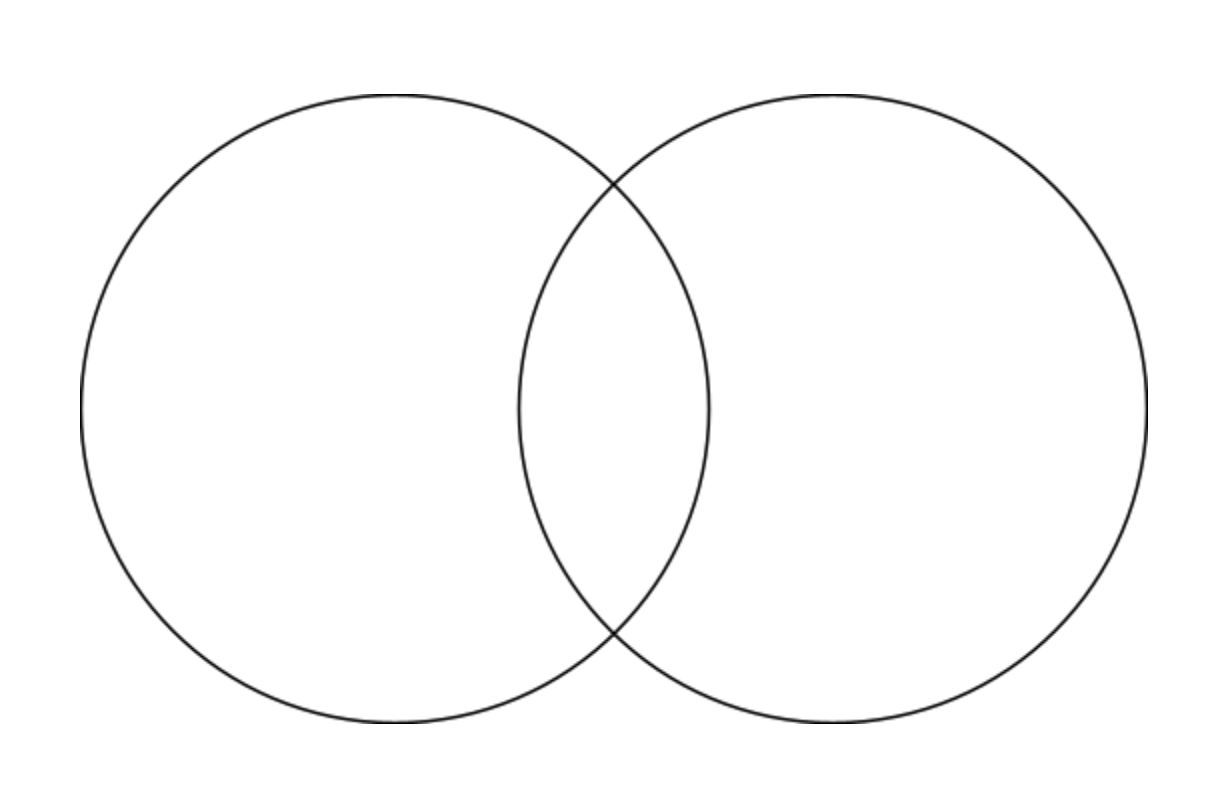
\includegraphics[width=0.6\textwidth]{venn-diagram}
      \centering
    \end{figure}

    In the above diagram, we assume the left circle corresponds to set $A$ and the
      right circle corresponds to $B$.
    The the possible sets we can make via the specified operators are:

    \begin{itemize}
      \item $A - B$, the left circle excluding the overlapping region.
      \item $A \cap B$, the overlapping region.
      \item $B - A$, the right circle excluding the overlapping region.
      \item $(A \cup B) \cap A$, the left circle.
      \item $(A \cup B) \cap B$, the right circle.
      \item $(A - B) \cup (B - A)$, the symmetric difference.
      \item $A \cup B$, the entire diagram.
    \end{itemize}
  \end{proof}

\subsection{\verified{Exercise 2.19}}%
\hyperlabel{sub:exercise-2.19}

  Is $\powerset{(A - B)}$ always equal to $\powerset{A} - \powerset{B}$?
  Is it ever equal to $\powerset{A} - \powerset{B}$?

  \code*{Bookshelf/Enderton/Set/Chapter\_2}
    {Enderton.Set.Chapter\_2.exercise\_2\_19}

  \begin{proof}
    Let $A$ and $B$ be arbitrary sets.
    We show (i) that $\emptyset \in \powerset{(A - B})$ and (ii)
      $\emptyset \not\in \powerset{A} - \powerset{B}$.

    \paragraph{(i)}%
    \hyperlabel{par:exercise-2.19-i}

      By definition of the \nameref{ref:power-set},
        $$\powerset{(A - B)} = \{ x \mid x \subseteq A - B \}.$$
      But $\emptyset$ is a subset of \textit{every} set.
      Thus $\emptyset \in \powerset{(A - B)}$.

    \paragraph{(ii)}%

      By the same reasoning found in \nameref{par:exercise-2.19-i},
        $\emptyset \in \powerset{A}$ and $\emptyset \in \powerset{B}$.
      But then, by definition of the relative complement,
        $\emptyset \not\in \powerset{A} - \powerset{B}$.

    \paragraph{Conclusion}%

      By the \nameref{ref:extensionality-axiom}, the two sets are never equal.

  \end{proof}

\subsection{\verified{Exercise 2.20}}%
\hyperlabel{sub:exercise-2.20}

  Let $A$, $B$, and $C$ be sets such that $A \cup B = A \cup C$ and
    $A \cap B = A \cap C$.
  Show that $B = C$.

  \code*{Bookshelf/Enderton/Set/Chapter\_2}
    {Enderton.Set.Chapter\_2.exercise\_2\_20}

  \begin{proof}
    Let $A$, $B$, and $C$ be arbitrary sets.
    By the \nameref{ref:extensionality-axiom}, $B = C$ if and only if for all
      sets $x$, $x \in B \iff x \in C$.
    We prove both directions of this biconditional.

    \paragraph{($\Rightarrow$)}%

      Suppose $x \in B$.
      Then there are two cases to consider:

      \subparagraph{Case 1}%

        Assume $x \in A$.
        Then $x \in A \cap B$.
        By hypothesis, $A \cap B = A \cap C$.
        Thus $x \in A \cap C$ immediately implying $x \in C$.

      \subparagraph{Case 2}%

        Assume $x \not\in A$.
        Then $x \in A \cup B$.
        By hypothesis, $A \cup B = A \cup C$.
        Thus $x \in A \cup C$.
        Since $x \not\in A$, it follows $x \in C$.

    \paragraph{($\Leftarrow$)}%

      Suppose $x \in C$.
      Then there are two cases to consider:

      \subparagraph{Case 1}%

        Assume $x \in A$.
        Then $x \in A \cap C$.
        By hypothesis, $A \cap B = A \cap C$.
        Thus $x \in A \cap B$, immediately implying $x \in B$.

      \subparagraph{Case 2}%

        Assume $x \not\in A$.
        Then $x \in A \cup C$.
        By hypothesis, $A \cup B = A \cup C$.
        Thus $x \in A \cup B$.
        Since $x \not\in A$, it follows $x \in B$.

  \end{proof}

\subsection{\verified{Exercise 2.21}}%
\hyperlabel{sub:exercise-2.21}

  Show that $\bigcup\; (A \cup B) = \bigcup A \cup \bigcup B$.

  \code*{Bookshelf/Enderton/Set/Chapter\_2}
    {Enderton.Set.Chapter\_2.exercise\_2\_21}

  \begin{proof}
    Let $A$ and $B$ be arbitrary sets.
    By the \nameref{ref:extensionality-axiom}, the specified equality holds if
      and only if for all sets $x$,
      $$x \in \bigcup (A \cup B) \iff x \in \bigcup A \cup \bigcup B.$$
    We prove both directions of this biconditional.

    \paragraph{($\Rightarrow$)}%

      Suppose $x \in \bigcup (A \cup B)$.
      By definition of the union of sets, there exists some $b \in A \cup B$
        such that $x \in b$.
      If $b \in A$, then $x \in \bigcup A$ and $x \in \bigcup A \cup \bigcup B$.
      Alternatively, if $b \in B$, then $x \in \bigcup B$ and
        $x \in \bigcup A \cup \bigcup B$.
      Regardless, $x$ is in the target set.

    \paragraph{($\Leftarrow$)}%

      Suppose $x \in \bigcup A \cup \bigcup B$.
      Then $x \in \bigcup A$ or $x \in \bigcup B$.
      WLOG, suppose $x \in \bigcup A$.
      By definition of the union of sets, there exists some $b \in A$ such that
        $x \in b$.
      But then $b \in A \cup B$ meaning $x$ is also a member of
        $\bigcup (A \cup B)$.

  \end{proof}

\subsection{\verified{Exercise 2.22}}%
\hyperlabel{sub:exercise-2.22}

  Show that if $A$ and $B$ are nonempty sets, then
    $\bigcap (A \cup B) = \bigcap A \cap \bigcap B$.

  \code*{Bookshelf/Enderton/Set/Chapter\_2}
    {Enderton.Set.Chapter\_2.exercise\_2\_22}

  \begin{proof}
    Let $A$ and $B$ be arbitrary, nonempty sets.
    By the \nameref{ref:extensionality-axiom}, the specified equality holds if
      and only if for all sets $x$,
      \begin{equation}
        \hyperlabel{sub:exercise-2.22-eq1}
        x \in \bigcap (A \cup B) \iff x \in \bigcap A \cap \bigcap B.
      \end{equation}
    We prove both directions of this biconditional.

    \paragraph{($\Rightarrow$)}%

      Suppose $x \in \bigcap (A \cup B)$.
      Then for all $b \in A \cup B$, $x \in B$.
      In other words, for every member $b_1$ of $A$ and every member $b_2$ of
        $B$, $x$ is a member of both $b_1$ and $b_2$.
      But that implies $x \in \bigcap A$ and $x \in \bigcap B$.

    \paragraph{($\Leftarrow$)}%

      Suppose $x \in \bigcap A \cap \bigcap B$.
      That is, $x \in \bigcap A$ and $x \in \bigcap B$.
      By definition of the intersection of sets, forall sets $b$, if $b \in A$,
        then $x \in b$.
      Likewise, if $b \in B$, then $x \in b$.
      In other words, if $b$ is a member of either $A$ or $B$, $x \in b$.
      That immediately implies $x \in \bigcap (A \cup B$.

  \end{proof}

\subsection{\unverified{Exercise 2.23}}%
\hyperlabel{sub:exercise-2.23}

  Show that if $\mathscr{B}$ is nonempty, then
    $A \cup \bigcap \mathscr{B} =
      \bigcap\; \{A \cup X \mid X \in \mathscr{B} \}$.

  \begin{proof}
    Refer to \nameref{sub:general-distributive-laws}.
  \end{proof}

\subsection{\verified{Exercise 2.24a}}%
\hyperlabel{sub:exercise-2.24a}

  Show that if $\mathscr{A}$ is nonempty, then
    $\powerset{\bigcap\mathscr{A}} =
      \bigcap\; \{\powerset{X} \mid X \in \mathscr{A} \}$.

  \code*{Bookshelf/Enderton/Set/Chapter\_2}
    {Enderton.Set.Chapter\_2.exercise\_2\_24a}

  \begin{proof}
    Suppose $\mathscr{A}$ is a nonempty set.
    Then $\bigcap \mathscr{A}$ is well-defined.
    Therefore
      \begin{align*}
        \powerset{\bigcap\mathscr{A}}
          & = \{ x \mid x \subseteq \bigcap \mathscr{A} \}
            & \textref{ref:power-set} \\
          & = \{ x \mid x \subseteq
            \{ y \mid \forall X \in \mathscr{A}, y \in X \} \}
            & \text{def'n intersection} \\
          & = \{ x \mid \forall t \in x,
            t \in \{ y \mid \forall X \in \mathscr{A}, y \in X \} \}
            & \text{def'n subset} \\
          & = \{ x \mid \forall t \in x,
            (\forall X \in \mathscr{A}, t \in X) \} \\
          & = \{ x \mid \forall X \in \mathscr{A},
            (\forall t \in x, t \in X) \} \\
          & = \{ x \mid \forall X \in \mathscr{A}, x \subseteq X \} \\
          & = \{ x \mid \forall X \in \mathscr{A}, x \in \powerset{X} \}
            & \textref{ref:power-set-axiom} \\
          & = \{ x \mid
            \forall t \in \{ \powerset{X} \mid X \in \mathscr{A} \}, x \in t \} \\
          & = \bigcap\; \{\powerset{X} \mid X \in \mathscr{A}\}.
      \end{align*}
  \end{proof}

\subsection{\verified{Exercise 2.24b}}%
\hyperlabel{sub:exercise-2.24b}

  Show that
    \begin{equation}
      \hyperlabel{sub:exercise-2.24b-eq1}
      \bigcup\; \{ \powerset{X} \mid X \in \mathscr{A} \} \subseteq
        \powerset{\bigcup\mathscr{A}}.
    \end{equation}
  Under what conditions does equality hold?

  \code*{Bookshelf/Enderton/Set/Chapter\_2}
    {Enderton.Set.Chapter\_2.exercise\_2\_24b}

  \begin{proof}
    We first prove \eqref{sub:exercise-2.24b-eq1}.
    Let $x \in \bigcup\; \{ \powerset{X} \mid X \in \mathscr{A} \}$.
    By definition of the union of sets,
      $(\exists X \in \mathscr{A}), x \in \powerset{X}$.
    By definition of the \nameref{ref:power-set}, $x \subseteq X$.
    By \nameref{sub:exercise-2.3}, $X \subseteq \bigcup \mathscr{A}$.
    Therefore $x \subseteq \bigcup \mathscr{A}$, proving
      $x \in \powerset{\mathscr{A}}$ as expected.

    \suitdivider

    \noindent
    We show $\powerset{\bigcup A} \subseteq 
      \bigcup\;\{ \powerset{X} \mid X \in \mathscr{A} \}$ if and only if
      $\bigcup\mathscr{A} \in \mathscr{A}$.

    \paragraph{($\Rightarrow$)}%

      Suppose $\powerset{\bigcup\mathscr{A}} \subseteq
        \bigcup\;\{ \powerset{X} \mid X \in \mathscr{A} \}$.
      By definition of the \nameref{ref:power-set},
        $\bigcup\mathscr{A} \in \powerset{\bigcup\mathscr{A}}$.
      By hypothesis, $\bigcup\mathscr{A} \in 
        \bigcup\;\{ \powerset{X} \mid X \in \mathscr{A} \}$.
      By definition of the union of sets, there exists some $X \in \mathscr{A}$
        such that $\bigcup\mathscr{A} \in \powerset{X}$.
      That is, $\bigcup\mathscr{A} \subseteq X$.
      But $\bigcup\mathscr{A}$ cannot be a proper subset of $X$ since
        $X \in \mathscr{A}$.
      Thus $\bigcup\mathscr{A} = X$.
      This proves $\bigcup\mathscr{A} \in
        \bigcup\;\{ \powerset{X} \mid X \in \mathscr{A} \}$.

    \paragraph{($\Leftarrow$)}%

      Suppose $\bigcup\mathscr{A} \in A$.
      Let $x \in \powerset{\bigcup\mathscr{A}}$.
      Since $\bigcup\mathscr{A} \in \mathscr{A}$, it immediately follows that
        $x \in \{\powerset{X} \mid X \in \mathscr{A}\}$.

    \paragraph{Conclusion}%

      Equality follows immediately from this fact in conjunction with the proof
        of \eqref{sub:exercise-2.24b-eq1}.

  \end{proof}

\subsection{\verified{Exercise 2.25}}%
\hyperlabel{sub:exercise-2.25}

  Is $A \cup \bigcup \mathscr{B}$ always the same as
    $\bigcup\;\{ A \cup X \mid X \in \mathscr{B} \}$?
  If not, then under what conditions does equality hold?

  \code*{Bookshelf/Enderton/Set/Chapter\_2}
    {Enderton.Set.Chapter\_2.exercise\_2\_25}

  \begin{proof}
    We prove that
      \begin{equation}
        \hyperlabel{sub:exercise-2.25-eq1}
        A \cup \bigcup \mathscr{B} =
          \bigcup\;\{ A \cup X \mid X \in \mathscr{B} \}
      \end{equation}
      if and only if $A = \emptyset$ or $\mathscr{B} \neq \emptyset$.
    We prove both directions of this biconditional.

    \paragraph{($\Rightarrow$)}%

      Suppose \eqref{sub:exercise-2.25-eq1} holds true.
      There are two cases to consider:

      \subparagraph{Case 1}%

        Suppose $B \neq \emptyset$.
        Then $A = \emptyset \lor \mathscr{B} \neq \emptyset$ holds trivially.

      \subparagraph{Case 2}%

        Suppose $B = \emptyset$.
        Then $$A \cup \bigcup \mathscr{B} = A \cup \bigcup \emptyset = A$$ and
          $$
            \bigcup\;\{ A \cup X \mid X \in \mathscr{B} \}
              = \bigcup \emptyset \\
              = \emptyset.
          $$
        Then by hypothesis \eqref{sub:exercise-2.25-eq1}, $A = \emptyset$.
        Then $A = \emptyset \lor \mathscr{B} \neq \emptyset$ holds trivially.

    \paragraph{($\Leftarrow$)}%

      Suppose $A = \emptyset$ or $\mathscr{B} \neq \emptyset$.
      There are two cases to consider:

      \paragraph{Case 1}%

        Suppose $A = \emptyset$.
        Then $A \cup \bigcup \mathscr{B} = \bigcup{\mathscr{B}}$.
        Likewise,
          $$
            \bigcup \{ A \cup X \mid X \in \mathscr{B} \}
              = \bigcup \{ X \mid X \in \mathscr{B} \} \\
              = \bigcup \mathscr{B}.
          $$
        Therefore \eqref{sub:exercise-2.25-eq1} holds.

      \paragraph{Case 2}%

        Suppose $B \neq \emptyset$.
        Then
          \begin{align*}
            A \cup \bigcup\mathscr{B}
              & = \{ x \mid x \in A \lor x \in \bigcup\mathscr{B} \} \\
              & = \{ x \mid x \in A \lor (\exists b \in \mathscr{B}) x \in b \} \\
              & = \{ x \mid (\exists b \in \mathscr{B}) x \in A \lor x \in b \} \\
              & = \{ x \mid (\exists b \in \mathscr{B}) x \in A \cup b \} \\
              & = \{ x \mid x \in \bigcup \{ A \cup X \mid X \in \mathscr{B} \} \\
              & = \bigcup \{ A \cup X \mid X \in \mathscr{B} \}.
          \end{align*}
        Therefore \eqref{sub:exercise-2.25-eq1} holds.

  \end{proof}

\chapter{Relations and Functions}%
\hyperlabel{chap:relations-functions}

\section{Ordered Pairs}%
\hyperlabel{sec:ordered-pairs}

\subsection{\verified{Theorem 3A}}%
\hyperlabel{sub:theorem-3a}

  \begin{theorem}[3A]
    For any sets $x$, $y$, $u$, and $v$,
      \begin{equation}
        \hyperlabel{sub:theorem-3a-eq1}
        \tuple{u, v} = \tuple{x, y} \iff u = x \land v = y.
      \end{equation}
  \end{theorem}

  \code{Bookshelf/Enderton/Set/Chapter\_3}
    {Enderton.Set.Chapter\_3.OrderedPair.ext\_iff}

  \begin{proof}
    Let $x$, $y$, $u$, and $v$ be arbitrary sets.

    \paragraph{($\Leftarrow$)}%

      This follows trivially.

    \paragraph{($\Rightarrow$)}%

      Suppose $\tuple{u, v} = \tuple{x, y}$.
      Then, by definition of an \nameref{ref:ordered-pair},
        \begin{equation}
          \hyperlabel{sub:theorem-3a-eq2}
          \{\{u\}, \{u, v\}\} = \{\{x\}, \{x, y\}\}.
        \end{equation}
      By the \nameref{ref:extensionality-axiom}, it follows
        $\{u\} \in \{\{x\}, \{x, y\}\}$ and
        $\{u, v\} \in \{\{x\}, \{x, y\}\}$.
      That is,
        $$\{u\} = \{x\} \quad\text{or}\quad \{u\} = \{x, y\}$$
        and
        $$\{u, v\} = \{x\} \quad\text{or}\quad \{u, v\} = \{x, y\}.$$
      There are 4 cases to consider:

      \paragraph{Case 1}%

        Suppose $\{u\} = \{x\}$ and $\{u, v\} = \{x\}$.
        The former identity implies $u = x$.
        The latter identity implies $u = v = x$.
        Then \eqref{sub:theorem-3a-eq2} simplifies to
          $$\{\{u\}\} = \{\{x\}, \{x, y\}\},$$ meaning $x = y$.
        Thus $v = y$ as well.

      \paragraph{Case 2}%

        Suppose $\{u\} = \{x\}$ and $\{u, v\} = \{x, y\}$.
        The former identity implies $u = x$.
        Substituting into the latter identity yields $\{u, v\} = \{u, y\}$.
        This holds if and only if $v = y$.

      \paragraph{Case 3}%

        Suppose $\{u\} = \{x, y\}$ and $\{u, v\} = \{x\}$.
        The former identity implies $x = y = u$.
        Substituting into the latter yields $\{u, v\} = \{u\}$.
        Thus $u = v$ which in turn implies $v = y$.

      \paragraph{Case 4}%
        Suppose $\{u\} = \{x, y\}$ and $\{u, v\} = \{x, y\}$.
        The former identity implies $x = y = u$.
        Substituting into the latter yields $\{u, v\} = \{u\}$.
        This implies $v = u$ which in turn implies $v = y$.

      \paragraph{Conclusion}%

        These cases are exhaustive and each implies that $u = x$ and $v = y$.

  \end{proof}

\subsection{\verified{Lemma 3B}}%
\hyperlabel{sub:lemma-3b}

  \begin{lemma}[3B]
    If $x \in C$ and $y \in C$, then $\tuple{x, y} \in \powerset{\powerset{C}}$.
  \end{lemma}

  \code{Bookshelf/Enderton/Set/Chapter\_3}
    {Enderton.Set.Chapter\_3.lemma\_3b}

  \begin{proof}
    Let $C$ be an arbitrary set and $x, y \in C$.
    Then, by definition of the \nameref{ref:power-set},
      $\{x\}$ and $\{x, y\}$ are members of $\powerset{C}$.
    Likewise, $\{\{x\}, \{x, y\}\}$ is a member of $\powerset{\powerset{C}}$.
    By definition of an \nameref{ref:ordered-pair},
      $\tuple{x, y} = \{\{x\}, \{x, y\}\}$.
    This concludes our proof.
  \end{proof}

\subsection{\unverified{Corollary 3C}}%
\hyperlabel{sub:corollary-3c}

  \begin{theorem}[3C]
    For any sets $A$ and $B$, there is a set whose members are exactly the
      pairs $\tuple{x, y}$ with $x \in A$ and $y \in B$.
  \end{theorem}

  \lean{Mathlib/SetTheory/ZFC/Basic}{Set.prod}

  \begin{proof}
    Define $C = A \cup B$.
    Then for all $x \in A$ and for all $y \in B$, $x$ and $y$ are both in $C$.
    By \nameref{sub:lemma-3b}, it follows that
      $\tuple{x, y} \in \powerset{\powerset{C}}$.
    The \nameref{ref:power-set-axiom} indicates $\powerset{\powerset{C}}$ is
      indeed a set.
    Therefore the \nameref{ref:subset-axioms} are applicable.
    This implies the existence of a set $D$ such that
      $$\forall z, (z \in D \iff z \in \powerset{\powerset{C}} \land
        (\exists x, \exists y, x \in A \land y \in B \land
          z = \tuple{x, y})).$$
    By construction $D$ is the set whose members are exactly the pairs
      $\tuple{x, y}$ with $x \in A$ and $y \in B$.
  \end{proof}

\section{Relations}%
\hyperlabel{sec:relations}

\subsection{\verified{Theorem 3D}}%
\hyperlabel{sub:theorem-3d}

  \begin{theorem}[3D]
    If $\tuple{x, y} \in A$, then $x$ and $y$ belong to $\bigcup\bigcup A$.
  \end{theorem}

  \code{Bookshelf/Enderton/Set/Chapter\_3}
    {Enderton.Set.Chapter\_3.theorem\_3d}

  \begin{proof}
    Let $A$ be a set and $\tuple{x, y} \in A$.
    By definition of an \nameref{ref:ordered-pair},
      $$\tuple{x, y} = \{\{x\}, \{x, y\}\}.$$
    By \nameref{sub:exercise-2.3}, $\{\{x\}, \{x, y\}\} \subseteq \bigcup A$.
    Then $\{x, y\} \in \bigcup A$.
    Another application of \nameref{sub:exercise-2.3} implies
      $\{x, y\} \subseteq \bigcup\bigcup A$.
    Therefore $x, y \in \bigcup\bigcup A$.
  \end{proof}

\section{Functions}%
\hyperlabel{sec:functions}

\subsection{\verified{Theorem 3E}}%
\hyperlabel{sub:theorem-3e}

  \begin{theorem}[3E]
    For a set $F$, $\dom{(F^{-1})} = \ran{F}$ and $\ran{(F^{-1})} = \dom{F}$.
    For a relation $F$, $(F^{-1})^{-1} = F$.
  \end{theorem}

  \code{Bookshelf/Enderton/Set/Relation}
    {Set.Relation.dom\_inv\_eq\_ran\_self}

  \code{Bookshelf/Enderton/Set/Relation}
    {Set.Relation.ran\_inv\_eq\_dom\_self}

  \code{Bookshelf/Enderton/Set/Relation}
    {Set.Relation.inv\_inv\_eq\_self}

  \begin{proof}
    We prove that (i) $\dom{(F^{-1})} = \ran{F}$, (ii)
      $\ran{(F^{-1})} = \dom{F}$, and (iii) $(F^{-1})^{-1} = F$.

    \paragraph{(i)}%

      By definition of the \nameref{ref:domain}, $x \in \dom{(F^{-1})}$ if and
        only if there exists some $y$ such that $\tuple{x, y} \in F^{-1}$.
      By definition of the \nameref{ref:inverse} of a set,
        $\tuple{y, x} \in F$.
      By definition of the \nameref{ref:range}, $x \in \ran{F}$.
      Since each step holds biconditionally, it follows
        $\dom{(F^{-1})} = \ran{F}$ as expected.

    \paragraph{(ii)}%

      By definition of the \nameref{ref:range}, $x \in \ran{(F^{-1})}$ if and
        only if there exists some $t$ such that $\tuple{t, x} \in F^{-1}$.
      By definition of the \nameref{ref:inverse} of a set,
        $\tuple{x, t} \in F$.
      By definition of the \nameref{ref:domain}, $x \in \dom{F}$.
      Since each step holds biconditionally, it follows
        $\ran{(F^{-1})} = \dom{F}$.

    \paragraph{(iii)}%

      By definition of the \nameref{ref:inverse} of a set,
        \begin{align*}
          (F^{-1})^{-1}
            & = \{\tuple{u, v} \mid \tuple{v, u} \in F^{-1}\} \\
            & = \{\tuple{u, v} \mid \tuple{u, v} \in F\} \\
            & = F.
        \end{align*}

  \end{proof}

\subsection{\verified{Theorem 3F}}%
\hyperlabel{sub:theorem-3f}

  \begin{theorem}[3F]
    For a set $F$, $F^{-1}$ is a function iff $F$ is single-rooted.
    A relation $F$ is a function iff $F^{-1}$ is single-rooted.
  \end{theorem}

  \code{Bookshelf/Enderton/Set/Relation}
    {Set.Relation.single\_valued\_inv\_iff\_single\_rooted\_self}

  \code{Bookshelf/Enderton/Set/Relation}
    {Set.Relation.single\_valued\_self\_iff\_single\_rooted\_inv}

  \begin{proof}
    We prove that (i) any set $F$, $F^{-1}$ is a function iff $F$ is
      single-rooted and (ii) any relation $F$ is a function iff $F^{-1}$ is
      single-rooted.

    \paragraph{(i)}%
    \hyperlabel{par:theorem-3f-i}

      Let $F$ be any set.

      \subparagraph{($\Rightarrow$)}%

        Suppose $F^{-1}$ is a \nameref{ref:function}.
        By definition, for each $x \in \dom{(F^{-1})}$, there is only one $y$
          such that $\tuple{x, y} \in F^{-1}$.
        By definition of the \nameref{ref:inverse} of $F$,
          $F^{-1} = \{\tuple{u, v} \mid vFu\}$.
        Then for each $x \in \ran{F}$, there exists exactly one $y$ such that
          $\tuple{y, x} \in F$.
        This definitionally means $F$ is single-rooted.

      \subparagraph{($\Leftarrow$)}%

        Suppose $F$ is single-rooted.
        By definition, for each $x \in \ran{F}$, there is only one $t$ such that
          $\tuple{t, x} \in F$.
        By definition of the \nameref{ref:inverse} of $F$,
          $F^{-1} = \{\tuple{u, v} \mid vFu\}$.
        Then for each $x \in \dom{(F^{-1})}$ there exists exactly one $t$ such
          that $\tuple{x, t} \in F^{-1}$.
        This definitionally means $F^{-1}$ is a function.

    \paragraph{(ii)}%

      Let $F$ be a \nameref{ref:relation}.

      \subparagraph{($\Rightarrow$)}%

        Suppose $F$ is a function.
        By \nameref{sub:theorem-3e}, $F = (F^{-1})^{-1}$.
        Then by \nameref{par:theorem-3f-i}, $F^{-1}$ is single-rooted.

      \subparagraph{($\Leftarrow$)}%

        Suppose $F^{-1}$ is single-rooted.
        Then by \nameref{par:theorem-3f-i}, $(F^{-1})^{-1}$ is a function.
        By \nameref{sub:theorem-3e}, $(F^{-1})^{-1} = F$.
        Thus $F$ is a function.

  \end{proof}

\subsection{\verified{One-to-One Inverse}}%
\hyperlabel{sub:one-to-one-inverse}

  \begin{lemma}
    For any one-to-one function $F$, $F^{-1}$ is also a one-to-one function.
  \end{lemma}

  \code{Bookshelf/Enderton/Set/Relation}
    {Set.Relation.one\_to\_one\_self\_iff\_one\_to\_one\_inv}

  \begin{proof}
    We prove that (i) $F^{-1}$ is a function and (ii) $F^{-1}$ is single-rooted.

    \paragraph{(i)}%
    \hyperlabel{par:lemma-1-i}

      By hypothesis, $F$ is one-to-one.
      This means it is single-rooted, i.e. for all $x \in \ran{F}$, there exists
        exactly one $t$ such that $\tuple{t, x} \in F$.
      By definition of the \nameref{ref:inverse} of $F$,
        $\tuple{x, t} \in F^{-1}$.
      But then for all $x \in \dom{(F^{-1})}$, there exists exactly one $t$ such
        that $\tuple{x, t} \in F^{-1}$.
      Thus $F^{-1}$ is a function.

    \paragraph{(ii)}%
    \hyperlabel{par:lemma-1-ii}

      By hypothesis, $F$ is single-valued.
      That is, for all $x \in \dom{F}$, there exists exactly one $y$ such that
        $\tuple{x, y} \in F$.
      By definition of the \nameref{ref:inverse} of $F$,
        $\tuple{y, x} \in F^{-1}$.
      But then for all $x \in \ran{(F^{-1})}$, there exists exactly one $y$ such
        that $\tuple{y, x} \in F^{-1}$.
      Thus $F^{-1}$ is single-rooted.

    \paragraph{Conclusion}%

      By \nameref{par:lemma-1-i} and \nameref{par:lemma-1-ii}, $F^{-1}$ is
        a one-to-one function.

  \end{proof}

\subsection{\verified{Theorem 3G}}%
\hyperlabel{sub:theorem-3g}

  \begin{theorem}[3G]
    Assume that $F$ is a one-to-one function.
    If $x \in \dom{F}$, then $F^{-1}(F(x)) = x$.
    If $y \in \ran{F}$, then $F(F^{-1}(y)) = y$.
  \end{theorem}

  \code{Bookshelf/Enderton/Set/Chapter\_3}
    {Enderton.Set.Chapter\_3.theorem\_3g\_i}

  \code{Bookshelf/Enderton/Set/Chapter\_3}
    {Enderton.Set.Chapter\_3.theorem\_3g\_ii}

  \begin{proof}
    Suppose $F$ is a one-to-one \nameref{ref:function}.
    Then \nameref{sub:one-to-one-inverse} indicates $F^{-1}$ is a one-to-one
      function with domain $\ran{F}$ and range $\dom{F}$.
    For all $x \in \dom{F}$, $\tuple{x, F(x)} \in F$.
    Then $\tuple{F(x), x} \in F^{-1}$.
    Since $F^{-1}$ is single-valued, $F^{-1}(F(x)) = x$.
    For all $y \in \ran{F}$, $\tuple{y, F^{-1}(y)} \in F^{-1}$.
    Then $\tuple{F^{-1}(y), y} \in F$.
    Since $F$ is single-valued, $F(F^{-1}(y)) = y$.
  \end{proof}

\subsection{\verified{Theorem 3H}}%
\hyperlabel{sub:theorem-3h}

  \begin{theorem}[3H]
    Assume that $F$ and $G$ are functions.
    Then $F \circ G$ is a function, its domain is
      \begin{equation}
        \hyperlabel{sub:theorem-3h-eq1}
        \{x \in \dom{G} \mid G(x) \in \dom{F}\},
      \end{equation}
      and for $x$ in its domain, $(F \circ G)(x) = F(G(x))$.
  \end{theorem}

  \code{Bookshelf/Enderton/Set/Relation}
    {Set.Relation.single\_valued\_comp\_is\_single\_valued}

  \code{Bookshelf/Enderton/Set/Chapter\_3}
    {Enderton.Set.Chapter\_3.theorem\_3h\_dom}

  \begin{proof}
    Let $F$ and $G$ be \nameref{ref:function}s.
    By definition of the \nameref{ref:composition} of $F$ and $G$,
      \begin{equation}
        \hyperlabel{sub:theorem-3h-eq2}
        F \circ G = \{\tuple{u, v} \mid \exists t(uGt \land tFv)\}.
      \end{equation}
    By construction, $F \circ G$ is a relation.
    By the definition of the \nameref{ref:domain} of a relation,
      $x \in \dom{(F \circ G)}$ if and only if there exists some $y$ such that
      $\tuple{x, y} \in F \circ G$.
    We prove that (i) $F \circ G$ is a function with domain satisfying
      \eqref{sub:theorem-3h-eq1}, and (ii) $(F \circ G)(x) = F(G(x))$.

    \paragraph{(i)}%
    \hyperlabel{par:theorem-3h-i}

      By \eqref{sub:theorem-3h-eq2}, there exists some $t$ such that
        $\tuple{x, t} \in G$ and $\tuple{t, y} \in F$.
      Since $G$ is single-valued, $t$ is uniquely determined by $x$.
      Since $F$ is single-valued, $y$ is uniquely determined by $t$.
      Therefore, by transitivity, $y$ is uniquely determined by $x$.
      Thus $F \circ G$ is single-valued, i.e. $F \circ G$ is a function.

      Furthermore, by definition of function application, $t = G(x)$.
      Thus $$\tuple{x, G(x)} \in G \quad\text{and}\quad \tuple{G(x), y} \in F.$$
      This immediately implies \eqref{sub:theorem-3h-eq1} holds true.

    \paragraph{(ii)}%

      Let $x \in \dom{(F \circ G)}$.
      By definition, $\tuple{x, (F \circ G)(x)} \in F \circ G$.
      Then \eqref{sub:theorem-3h-eq2} implies $(F \circ G)(x)$ satisfies
        $\tuple{G(x), (F \circ G)(x)} \in F$.
      This is equivalent to saying $F(G(x)) = (F \circ G)(x)$ as expected.

  \end{proof}

\subsection{\verified{One-to-One Composition}}%
\hyperlabel{sub:one-to-one-composition}

  \begin{lemma}
    Let $F$ and $G$ be one-to-one functions.
    Then $F \circ G$ is also a one-to-one function.
  \end{lemma}

  \code{Bookshelf/Enderton/Set/Relation}
    {Set.Relation.one\_to\_one\_comp\_is\_one\_to\_one}

  \begin{proof}
    Let $F \colon B \rightarrow C$ and $G \colon A \rightarrow B$ be
      one-to-one \nameref{ref:function}s from sets $A$, $B$, and $C$.
    By definition of the \nameref{ref:composition} of functions,
      \begin{equation}
        \hyperlabel{sub:one-to-one-composition-eq1}
        F \circ G = \{\tuple{u, v} \mid \exists t(uGt \land tFv)\}.
      \end{equation}
    By \nameref{sub:theorem-3h}, $F \circ G$ is a function.

    All that remains is proving $F \circ G$ is one-to-one.
    Let $(F \circ G)(x_1) = (F \circ G)(x_2) = y$.
    By \eqref{sub:one-to-one-composition-eq1}, there exists some $t_1$ such that
      $x_1Gt_1$ and $t_1Fy$.
    Likewise, there exists some $t_2$ such that $x_2Gt_2$ and $t_2Fy$.
    Since $F$ is one-to-one, it follows $t_1 = t_2$.
    Then, since $G$ is also one-to-one, it follows $x_1 = x_2$.
    Hence $F \circ G$ is one-to-one.
  \end{proof}

\subsection{\verified{Theorem 3I}}%
\hyperlabel{sub:theorem-3i}

  \begin{theorem}[3I]
    For any sets $F$ and $G$, $$(F \circ G)^{-1} = G^{-1} \circ F^{-1}.$$
  \end{theorem}

  \code{Bookshelf/Enderton/Set/Relation}
    {Set.Relation.comp\_inv\_eq\_inv\_comp\_inv}

  \begin{proof}
    By definition of the \nameref{ref:composition} of $F$ and $G$,
      $$F \circ G = \{\tuple{u, v} \mid \exists t(uGt \land tFv)\}.$$
    By definition of the \nameref{ref:inverse} of a function,
      \begin{align*}
        (F \circ G)^{-1}
          & = \{\tuple{u, v} \mid \exists t (vGt \land tFu)\} \\
          & = \{\tuple{u, v} \mid \exists t (tFu \land vGt)\} \\
          & = \{\tuple{u, v} \mid
            \exists t \left[ u(F^{-1})t \land t(G^{-1})v \right]\} \\
          & = G^{-1} \circ F^{-1}.
      \end{align*}
  \end{proof}

\subsection{\pending{Theorem 3J}}%
\hyperlabel{sub:theorem-3j}

  \begin{theorem}[3J]
    Assume that $F \colon A \rightarrow B$, and that $A$ is nonempty.
    \begin{enumerate}[(a)]
      \item There exists a function $G \colon B \rightarrow A$
        (a "left inverse") such that $G \circ F$ is the identity function $I_A$
        on $A$ iff $F$ is one-to-one.
      \item There exists a function $H \colon B \rightarrow A$
        (a "right inverse") such that $F \circ H$ is the identity function $I_B$
        on $B$ iff $F$ maps $A$ \textit{onto} $B$.
    \end{enumerate}
  \end{theorem}

  \begin{proof}
    Let $F$ be a \nameref{ref:function} from nonempty set $A$ to set $B$.

    \paragraph{(a)}%

      We prove there exists a function $G \colon B \rightarrow A$ such that
        $G \circ F = I_A$ if and only if $F$ is one-to-one.

      \subparagraph{($\Rightarrow$)}%

        Let $G \colon B \rightarrow A$ such that $G \circ F = I_A$.
        All that remains is to prove $F$ is single-rooted.
        Let $y \in \ran{F}$.
        By definition of the \nameref{ref:range} of a function, there exists
          some $x_1$ such that $\tuple{x_1, y} \in F$.
        Suppose there exists a set $x_2$ such that $\tuple{x_2, y} \in F$.
        By hypothesis, $G(F(x_1)) = G(F(x_2))$ implies $I_A(x_1) = I_A(x_2)$.
        Thus $x_1 = x_2$.
        Therefore $F$ must be single-rooted.

      \subparagraph{($\Leftarrow$)}%

        Let $F$ be one-to-one.
        Since $A$ is nonempty, there exists some $a \in A$.
        Let $G \colon B \rightarrow A$ be given by
          $$G(y) = \begin{cases}
            F^{-1}(y) & \text{if } y \in \ran{F} \\
            a & \text{otherwise}.
          \end{cases}$$
        $G$ is a function by virtue of \nameref{sub:one-to-one-inverse} and
          choice of mapping for all values $y \not\in \ran{F}$.
        Furthermore, for all $x \in A$, $F(x) \in \ran{F}$.
        Thus $(G \circ F)(x) = G(F(x)) = F^{-1}(F(x)) = x$ by
          \nameref{sub:theorem-3g}.

    \paragraph{(b)}%

      We prove there exists a function $H \colon B \rightarrow A$ such that
        $F \circ H = I_A$ if and only if $F$ maps $A$ onto $B$.

      \subparagraph{($\Rightarrow$)}%

        Suppose $H \colon B \rightarrow A$ such that $F \circ H = I_A$.
        All that remains is to prove $\ran{F} = B$.
        Note that $\ran{F} \subseteq B$ by hypothesis.
        Let $y \in B$.
        But $F(H(y)) = y$ meaning $y \in \ran{F}$.
        Thus $B \subseteq \ran{F}$.
        Since $\ran{F} \subseteq B$ and $B \subseteq \ran{F}$, $\ran{F} = B$.

      \subparagraph{($\Leftarrow$)}%

        Suppose $F$ maps $A$ \textit{onto} $B$.
        By definition of maps onto, $\ran{F} = B$.
        Then for all $y \in B$, there exists some $x \in A$ such that
          $\tuple{x, y} \in F$.
        Notice though that $F^{-1}[\{y\}]$ may not be a singleton set.
        Then there is no obvious way to \textit{choose} an element from each
          preimage to form a function.
        By the \nameref{ref:axiom-of-choice-1}, there exists a function
          $H \subseteq F^{-1}$ such that $\dom{H} = \dom{F^{-1}} = B$.
        For all $y \in B$, $\tuple{y, H(y)} \in H \subseteq F^{-1}$
          meaning $\tuple{H(y), y} \in F$.
        Thus $F(H(y)) = y$ as expected.

  \end{proof}

\subsection{\unverified{Bijections are Two-Sided Inverses}}%
\hyperlabel{sub:bijections-two-sided-inverses}

  \begin{corollary}
    A function $f$ is a one-to-one correspondence if and only if it has a left
      and right inverse.
  \end{corollary}

  \begin{proof}
    By definition, a one-to-one correspondence $f$ between sets $A$ and $B$ must
      be both one-to-one and onto.
    By \nameref{sub:theorem-3j}, $f$ is one-to-one if and only if it has a left
      inverse.
    The same theorem states that $f$ is onto $B$ if and only if it has a right
      inverse.
  \end{proof}

\subsection{\verified{Theorem 3K(a)}}%
\hyperlabel{sub:theorem-3k-a}

  \begin{theorem}[3K(a)]
    The following hold for any sets. ($F$ need not be a function.)
    The image of a union is the union of the images:
      \begin{equation}
        \hyperlabel{sub:theorem-3k-a-eq1}
        \img{F}{A \cup B} = \img{F}{A} \cup \img{F}{B}
      \end{equation}
      and
      \begin{equation}
        \hyperlabel{sub:theorem-3k-a-eq2}
        \img{F}{\bigcup{\mathscr{A}}} =
          \bigcup\;\{\img{F}{A} \mid A \in \mathscr{A}\}.
      \end{equation}
  \end{theorem}

  \code{Bookshelf/Enderton/Set/Chapter\_3}
    {Enderton.Set.Chapter\_3.theorem\_3k\_a}

  \begin{proof}
    Let $F$, $A$, $B$, and $\mathscr{A}$ be arbitrary sets.
    We prove (i) \eqref{sub:theorem-3k-a-eq1} and (ii)
      \eqref{sub:theorem-3k-a-eq2}.

    \paragraph{(i)}%

      By definition of the \nameref{ref:image} of a set:
        \begin{align*}
          \img{F}{A \cup B}
            & = \{v \mid \exists u, u \in A \cup B \land uFv\} \\
            & = \{v \mid \exists u,
              (u \in A \land uFv) \lor (u \in B \land uFv)\} \\
            & = \{v \mid (\exists u \in A) uFv\} \cup
              \{v \mid (\exists u \in B) uFv\} \\
            & = \img{F}{A} \cup \img{F}{B}.
        \end{align*}

    \paragraph{(ii)}%

      We prove that both sides of \eqref{sub:theorem-3k-a-eq2} is a subset of
        the other.

      \subparagraph{($\subseteq$)}%

        Let $v \in \img{F}{\bigcup{\mathscr{A}}}$.
        By definition of the \nameref{ref:image} of a set, there exists a set
          $u$ such that $u \in \bigcup{\mathscr{A}} \land uFv$.
        Then, by definition of the union of sets, there exists some
          $A \in \mathscr{A}$ such that $u \in A$.
        Therefore $v \in \img{F}{A}$ meaning
          $v \in \bigcup\{\img{F}{A} \mid A \in \mathscr{A}\}$.

      \subparagraph{($\supseteq$)}%

        Let $v \in \bigcup\{\img{F}{A} \mid A \in \mathscr{A}\}$.
        Then there exists some $b \in \{\img{F}{A} \mid A \in \mathscr{A}\}$
          such that $v \in b$.
        In other words, there exists some $A \in \mathscr{A}$ such that
          $v \in b = \img{F}{A}$.
        By definition of the \nameref{ref:image} of a set, there exists a set
          $u$ such that $u \in A \land uFv$.
        But this implies that $u \in \bigcup{\mathscr{A}} \land uFv$.
        Therefore $v \in \img{F}{\bigcup{\mathscr{A}}}$.

  \end{proof}

\subsection{\verified{Theorem 3K(b)}}%
\hyperlabel{sub:theorem-3k-b}

  \begin{theorem}[3K(b)]
    The following hold for any sets. ($F$ need not be a function.)
    The image of an intersection is included in the intersection of the images:
      \begin{equation}
        \hyperlabel{sub:theorem-3k-b-eq1}
        \img{F}{A \cap B} \subseteq \img{F}{A} \cap \img{F}{B}
      \end{equation}
      and
      \begin{equation}
        \hyperlabel{sub:theorem-3k-b-eq2}
        \img{F}{\bigcap\mathscr{A}} \subseteq
          \bigcap\;\{\img{F}{A} \mid A \in \mathscr{A}\}.
      \end{equation}
      for nonempty $\mathscr{A}$.
    Equality holds if $F$ is single-rooted.
  \end{theorem}

  \code{Bookshelf/Enderton/Set/Chapter\_3}
    {Enderton.Set.Chapter\_3.theorem\_3k\_b\_i}

  \code{Bookshelf/Enderton/Set/Chapter\_3}
    {Enderton.Set.Chapter\_3.theorem\_3k\_b\_ii}

  \begin{proof}
    Let $F$, $A$, $B$ be arbitrary sets.
    Let $\mathscr{A}$ be a nonempty set.
    We first prove (i) \eqref{sub:theorem-3k-b-eq1} and (ii)
      \eqref{sub:theorem-3k-b-eq2}.
    Then, assuming $F$ is single-rooted, we prove both (iii)
      \eqref{sub:theorem-3k-b-eq1} and (iv) \eqref{sub:theorem-3k-b-eq2} hold
      under equality.

    \paragraph{(i)}%
    \hyperlabel{par:theorem-3k-b-i}

      Let $v \in \img{F}{A \cap B}$.
      By definition of the \nameref{ref:image} of a set,
        $\exists u \in A \cap B, uFv$.
      Then $u \in A \land uFv$ and $u \in B \land uFv$.
      Therefore $v \in \img{F}{A} \cap \img{F}{B}$.

    \paragraph{(ii)}%
    \hyperlabel{par:theorem-3k-b-ii}

      Let $v \in \img{F}{\bigcap{\mathscr{A}}}$.
      By definition of the \nameref{ref:image} of a set,
        $\exists u \in \bigcap{\mathscr{A}}, uFv$.
      Then $\exists u, (\forall A \in \mathscr{A}, u \in A) \land uFv$.
      This implies that $\forall A \in \mathscr{A}, \exists u \in A, uFv$.
      Then $\forall A \in \mathscr{A}, v \in \img{F}{A}$.
      Thus $v \in \bigcap\{\img{F}{A} \mid A \in \mathscr{A}\}$.

    \paragraph{(iii)}%

      Suppose $F$ is single-rooted.
      By \nameref{par:theorem-3k-b-i},
        $$\img{F}{A \cap B} \subseteq \img{F}{A} \cap \img{F}{B}.$$
      All that remains is showing
        $$\img{F}{A} \cap \img{F}{B} \subseteq \img{F}{A \cap B}.$$
      Let $v \in \img{F}{A} \cap \img{F}{B}$.
      Then $v \in \img{F}{A}$ and $v \in \img{F}{B}$.
      That is, $\exists u \in A, uFv$ and $\exists w \in B, wFv$.
      Since $F$ is single rooted, it follows $u = w$.
      Thus $u \in A \cap B \land uFv$ meaning $v \in \img{F}{A \cap B}$.

    \paragraph{(iv)}%

      Suppose $F$ is single-rooted.
      By \nameref{par:theorem-3k-b-ii},
        $$\img{F}{\bigcap\mathscr{A}} \subseteq
          \bigcap\;\{\img{F}{A} \mid A \in \mathscr{A}\}.$$
      All that remains is showing
        $$\bigcap\;\{\img{F}{A} \mid A \in \mathscr{A}\} \subseteq
          \img{F}{\bigcap\mathscr{A}}.$$
      Let $v \in \bigcap\;\{\img{F}{A} \mid A \in \mathscr{A}\}$.
      Then $\forall A \in \mathscr{A}, v \in \img{F}{A}$.
      By definition of the \nameref{ref:image} of a set,
        $\forall A \in \mathscr{A}, \exists u \in A, uFv$.
      Since $F$ is single-rooted and $\mathscr{A}$ is nonempty, it follows that
        $\exists u, (\forall A \in \mathscr{A}, u \in A) \land uFv$.
      Equivalently, $\exists u \in \bigcap{A}, uFv$.
      Thus $v \in \img{F}{\bigcap{A}}$.

  \end{proof}

\subsection{\verified{Theorem 3K(c)}}%
\hyperlabel{sub:theorem-3k-c}

  \begin{theorem}[3K(c)]
    The following hold for any sets. ($F$ need not be a function.)
    The image of a difference includes the difference of the images:
      \begin{equation}
        \hyperlabel{sub:theorem-3k-c-eq1}
        \img{F}{A} - \img{F}{B} \subseteq \img{F}{A - B}.
      \end{equation}
    Equality holds if $F$ is single-rooted.
  \end{theorem}

  \code{Bookshelf/Enderton/Set/Chapter\_3}
    {Enderton.Set.Chapter\_3.theorem\_3k\_c\_i}

  \code{Bookshelf/Enderton/Set/Chapter\_3}
    {Enderton.Set.Chapter\_3.theorem\_3k\_c\_ii}

  \begin{proof}
    We prove that (i) \eqref{sub:theorem-3k-c-eq1} holds and (ii) equality holds
      if $F$ is single-rooted.

    \paragraph{(i)}%
    \hyperlabel{par:theorem-3k-c-i}

      Let $v \in \img{F}{A} - \img{F}{B}$.
      By definition of the difference of two sets,
        $v \in \img{F}{A}$ and $v \not\in \img{F}{B}$.
      By definition of the \nameref{ref:image} of a set, there exists a set
        $u \in A$ such that $\tuple{u, v} \in F$.
      Likewise, $\forall w \in B, \tuple{w, v} \not\in F$.
      Thus $u \not\in B$, since otherwise we get an immediate contradiction.
      Therefore $u \in A - B$ meaning $v \in \img{F}{A - B}$.

    \paragraph{(ii)}%

      Suppose $F$ is single-rooted.
      By \nameref{par:theorem-3k-c-i},
        $$\img{F}{A} - \img{F}{B} \subseteq \img{F}{A - B}.$$
      All that remains is showing
        $$\img{F}{A - B} \subseteq \img{F}{A} - \img{F}{B}.$$
      Let $v \in \img{F}{A - B}$.
      By definition of the \nameref{ref:image} of a set, there exists a set
        $u \in A - B$ such that $uFv$.
      Then $u \in A$ and $u \not\in B$.
      The former membership relation implies $v \in \img{F}{A}$.
      The latter implies $v \not\in \img{F}{B}$ since $F$ being single-rooted
        would otherwise invoke an immediate contradiction.
      Thus $v \in \img{F}{A} - \img{F}{B}$.

  \end{proof}

\subsection{\verified{Corollary 3L}}%
\hyperlabel{sub:corollary-3l}

  \begin{theorem}[3L]
    For any function $G$ and sets $A$, $B$, and $\mathscr{A}$:
    \begin{align}
      \img{G^{-1}}{\bigcup{\mathscr{A}}}
        & = \bigcup\;\{\img{G^{-1}}{A} \mid A \in \mathscr{A}\},
        \hyperlabel{sub:corollary-3l-eq1} \\
      \img{G^{-1}}{\bigcap{\mathscr{A}}}
        & = \bigcap\;\{\img{G^{-1}}{A} \mid A \in \mathscr{A}\}
        \text{ for } \mathscr{A} \neq \emptyset,
        \hyperlabel{sub:corollary-3l-eq2} \\
      \img{G^{-1}}{A - B} & = \img{G^{-1}}{A} - \img{G^{-1}}{B}.
        \hyperlabel{sub:corollary-3l-eq3}
    \end{align}
  \end{theorem}

  \code{Bookshelf/Enderton/Set/Chapter\_3}
    {Enderton.Set.Chapter\_3.corollary\_3l\_i}

  \code{Bookshelf/Enderton/Set/Chapter\_3}
    {Enderton.Set.Chapter\_3.corollary\_3l\_ii}

  \code{Bookshelf/Enderton/Set/Chapter\_3}
    {Enderton.Set.Chapter\_3.corollary\_3l\_iii}

  \begin{proof}
    \nameref{sub:theorem-3k-a} implies \eqref{sub:corollary-3l-eq1}.
    Because the inverse of a function is always single-rooted,
      \nameref{sub:theorem-3k-b} implies \eqref{sub:corollary-3l-eq2}.
    Likewise \nameref{sub:theorem-3k-c} implies \eqref{sub:corollary-3l-eq3}.
  \end{proof}

\section{Equivalence Relations}%
\hyperlabel{sec:equivalence-relations}

\subsection{\verified{Theorem 3M}}%
\hyperlabel{sub:theorem-3m}

  \begin{theorem}[3M]
    If $R$ is a symmetric and transitive relation, then $R$ is an equivalence
      relation on $\fld{R}$.
  \end{theorem}

  \code{Bookshelf/Enderton/Set/Chapter\_3}
    {Enderton.Set.Chapter\_3.theorem\_3m}

  \begin{proof}
    Suppose $R$ is a \nameref{ref:symmetric} and \nameref{ref:transitive}
      \nameref{ref:relation}.
    By definition, the \nameref{ref:field} of $R$ is given by
      $\fld{R} = \dom{R} \cup \ran{R}$.
    An \nameref{ref:equivalence-relation} on $\fld{R}$ is, by definition, a
      binary relation \nameref{ref:reflexive} on $\fld{R}$, symmetric, and
      transitive.
    All that remains is to show $R$ is reflexive on $\fld{R}$.

    Let $x \in \fld{R}$.
    Then $x \in \dom{R}$ or $x \in \ran{R}$.
    If $x \in \dom{R}$, there exists some $y$ such that $xRy$.
    Since $R$ is symmetric, it follows $yRx$.
    Since $R$ is transitive, it follows $xRx$.
    If instead $x \in \ran{R}$, there exists some $t$ such that $tRx$.
    Since $R$ is symmetric, it follows $xRt$.
    Since $R$ is transitive, it follows $xRx$.
    Thus $R$ is reflexive on $\fld{R}$.
  \end{proof}

\subsection{\verified{Lemma 3N}}%
\hyperlabel{sub:lemma-3n}

  \begin{lemma}[3N]
    Assume that $R$ is an equivalence relation on $A$ and that $x$ and $y$
      belong to $A$.
    Then $$[x]_R = [y]_R \iff xRy.$$
  \end{lemma}

  \code{Bookshelf/Enderton/Set/Relation}
    {Set.Relation.neighborhood\_iff\_mem}

  \begin{proof}
    Suppose $R$ is an \nameref{ref:equivalence-relation} on set $A$.
    Let $x, y \in A$.

    \paragraph{($\Rightarrow$)}%

      Suppose $[x]_R = [y]_R$.
      Since $R$ is an equivalence relation, it is reflexive on $A$.
      Thus $yRy$ meaning $y \in [y]_R = \{t \mid yRt\}$.
      Since $[x]_R = [y]_R$, $y \in \{t \mid xRt\}$ as well.
      That is, $xRy$.

    \paragraph{($\Leftarrow$)}%

      Suppose $xRy$.
      We show $[x]_R \subseteq [y]_R$ and $[y]_R \subseteq [x]_R$.

      \subparagraph{($\subseteq$)}%

        Let $t \in [x]_R$.
        Then $xRt$.
        Since $R$ is symmetric, $xRy$ implies $yRx$.
        Since $R$ is transitive, $yRx$ and $xRt$ implies $yRt$.
        Thus $t \in [y]_R$.

      \subparagraph{($\supseteq$)}%

        Let $t \in [y]_R$.
        Then $yRt$.
        Since $R$ is transitive, $xRy$ and $yRt$ implies $xRt$.
        Thus $t \in [x]_R$.

  \end{proof}

\subsection{\verified{Theorem 3P}}%
\hyperlabel{sub:theorem-3p}

  \begin{theorem}[3P]
    Assume that $R$ is an equivalence relation on $A$.
    Then the set $\{[x]_R \mid x \in A\}$ of all equivalence classes is a
      partition of $A$.
  \end{theorem}

  \code{Bookshelf/Enderton/Set/Relation}
    {Set.Relation.modEquiv\_partition}

  \begin{proof}
    Let $\Pi = \{[x]_R \mid x \in A\}$.
    We show that (i) there are no empty sets in $\Pi$, (ii) no two different
      sets in $\Pi$ have any common elements and (iii) that each element of $A$
      is in some set in $\Pi$.

    \paragraph{(i)}%

      By construction, every element of $\Pi$ is of form $[x]_R$ for some
        $x \in A$.
      At the very least, $x \in A$ is also in $[x]_R$.
      Thus every element of $\Pi$ must be nonempty.

    \paragraph{(ii)}%

      Let $[x]_R, [y]_R \in \Pi$ be two different sets.
      We must show that $[x]_R \cap [y]_R = \emptyset$.
      For the sake of contradiction, suppose $[x]_R \cap [y]_R \neq \emptyset$.
      Let $z \in [x]_R \cap [y]_R$.
      Then $xRz$ and $yRz$.
      Since $R$ is an \nameref{ref:equivalence-relation} on $A$, it is
        \nameref{ref:symmetric} and \nameref{ref:transitive}.
      Then $zRy$ and $xRy$.
      By \nameref{sub:lemma-3n}, $xRy$ if and only if $[x]_R = [y]_R$,
        contradicting the distinctness of $[x]_R$ and $[y]_R$.
      Thus it follows $[x]_R \cap [y]_R] = \emptyset$.

    \paragraph{(iii)}%

      Let $x \in A$.
      Since $R$ is an \nameref{ref:equivalence-relation} on $A$, it follows
        $xRx$.
      Thus $x$ is a member of some set in $\Pi$, namely $[x]_R$.

  \end{proof}

\subsection{\unverified{Theorem 3Q}}%
\hyperlabel{sub:theorem-3q}

  \begin{theorem}[3Q]
    Assume that $R$ is an equivalence relation on $A$ and that
      $F \colon A \rightarrow A$.
    If $F$ is compatible with $R$, then there exists a unique
      $\hat{F} \colon A / R \rightarrow A / R$ such that
      \begin{equation}
        \hyperlabel{sub:theorem-3q-eq1}
        \hat{F}([x]_R) = [F(x)]_R \quad\text{for all } x \text{ in } A.
      \end{equation}
    If $F$ is not compatible with $R$, then no such $\hat{F}$ exists.
  \end{theorem}

  \begin{proof}
    Let $R$ be an \nameref{ref:equivalence-relation} on $A$ and
      $F \colon A \rightarrow A$.
    Suppose $F$ is \nameref{ref:compatible} with $R$.
    Next define \nameref{ref:relation} $\hat{F}$ to be
      $$\hat{F} = \{\tuple{[x]_R, [F(x)]_R} \mid x \in A\}.$$
    By construction $\hat{F}$ has domain $A / R$ and
      $\ran{\hat{F}} \subseteq A / R$.
    All that remains is proving $\hat{F}$ is single-valued.
    Let $[x_1]_R, [x_2]_R \in \dom{\hat{F}}$ such that $[x_1]_R = [x_2]_R$.
    By definition of $\hat{F}$, $\tuple{[x_1]_R, [F(x_1)]_R} \in \hat{F}$
      and $\tuple{[x_2]_R, [F(x_2)]_R} \in \hat{F}$.
    By \nameref{sub:lemma-3n}, $[x_1]_R = [x_2]_R$ implies $x_1Rx_2$.
    Since $F$ is compatible, $F(x_1)RF(x_2)$.
    Another application of \nameref{sub:lemma-3n} implies that
      $[F(x_1)]_R = [F(x_2)]_R$.
    Thus $\hat{F}$ is single-valued.

    Uniqueness follows immediately from the \nameref{ref:extensionality-axiom}.

    \suitdivider

    Suppose $F$ is not compatible with $R$.
    Then there exists some $x, y \in A$ such that $xRy$ and $\neg F(x)RF(y)$.
    By \nameref{sub:lemma-3n}, $[x]_R = [y]_R$.
    For the sake of contradiction, suppose a function $\hat{F}$ exists
      satisfying \eqref{sub:theorem-3q-eq1}.
    Then $\hat{F}([x]_R) = \hat{F}([y]_R)$ meaning $[F(x)]_R = [F(y)]_R$.
    Then \nameref{sub:lemma-3n} implies $F(x)RF(y)$, a contradiction.
    Therefore our original hypothesis must be incorrect.
    That is, there is no function $\hat{F}$ satisfying
      \eqref{sub:theorem-3q-eq1}.
  \end{proof}

\section{Ordering Relations}%
\hyperlabel{sec:ordering-relations}

\subsection{\verified{Theorem 3R}}%
\hyperlabel{sub:theorem-3r}

  \begin{theorem}[3R]
    Let $R$ be a linear ordering on $A$.
    \begin{enumerate}[(i)]
      \item There is no $x$ for which $xRx$.
      \item For distinct $x$ and $y$ in $A$, either $xRy$ or $yRx$ (but not both).
    \end{enumerate}
  \end{theorem}

  \code{Bookshelf/Enderton/Set/Chapter\_3}
    {Enderton.Set.Chapter\_3.theorem\_3r}

  \begin{proof}
    Suppose $R$ is a \nameref{ref:linear-ordering} on $A$.

    \paragraph{(i)}%

      Let $x \in A$.
      By definition, $R$ is \nameref{ref:trichotomous}.
      Then only one of $xRx$ and $x = x$ can hold.
      Since $x = x$ obviously holds, it follows $\tuple{x, x} \not\in R$.

    \paragraph{(ii)}%

      Let $x, y \in A$ such that $x \neq y$.
      By definition, $R$ is \nameref{ref:trichotomous}.
      Thus only one of $$xRy, \quad x = y, \quad yRx$$ hold.
      By hypothesis $x \neq y$ meaning either $xRy$ or $yRx$ (but not both).

  \end{proof}

\section{Exercises 3}%
\hyperlabel{sec:exercises-3}

\subsection{\verified{Exercise 3.1}}%
\hyperlabel{sub:exercise-3.1}

  Suppose that we attempted to generalize the Kuratowski definitions of ordered
    pairs to ordered triples by defining
    $$\tuple{x, y, z}^* = \{\{x\}, \{x, y\}, \{x, y, z\}\}.$$
  Show that this definition is unsuccessful by giving examples of objects
    $u$, $v$, $w$, $x$, $y$, $z$ with
    $\tuple{x, y, z}^* = \tuple{u, v, w}^*$ but with either
    $y \neq v$ or $z \neq w$ (or both).

  \code*{Bookshelf/Enderton/Set/Chapter\_3}
    {Enderton.Set.Chapter\_3.exercise\_3\_1}

  \begin{proof}
    Let $x = 1$, $y = 1$, and $z = 2$.
    Let $u = 1$, $v = 2$, and $w = 2$.
    Then
      \begin{align*}
        \tuple{x, y, z}^*
          & = \{\{x\}, \{x, y\}, \{x, y, z\}\} \\
          & = \{\{1\}, \{1, 1\}, \{1, 1, 2\}\} \\
          & = \{\{1\}, \{1, 2\}\}.
      \end{align*}
    Likewise
      \begin{align*}
        \tuple{u, v, w}^*
          & = \{\{u\}, \{u, v\}, \{u, v, w\}\} \\
          & = \{\{1\}, \{1, 2\}, \{1, 2, 2\}\} \\
          & = \{\{1\}, \{1, 2\}\}.
      \end{align*}
    Thus $\tuple{x, y, z}^* = \tuple{u, v, w}^*$ but $y \neq v$.
  \end{proof}

\subsection{\verified{Exercise 3.2a}}%
\hyperlabel{sub:exercise-3.2a}

  Show that $A \times (B \cup C) = (A \times B) \cup (A \times C)$.

  \code*{Bookshelf/Enderton/Set/Chapter\_3}
    {Enderton.Set.Chapter\_3.exercise\_3\_2a}

  \begin{proof}
    Let $A$, $B$, and $C$ be arbitrary sets.
    Then by \nameref{sub:corollary-3c} and the definition of the union of sets,
      \begin{align*}
        A \times (B \cup C)
          & = \{ \tuple{x, y} \mid x \in A \land y \in (B \cup C) \} \\
          & = \{ \tuple{x, y} \mid
            x \in A \land (y \in B \lor y \in C) \} \\
          & = \{ \tuple{x, y} \mid
            (x \in A \land y \in B) \lor (x \in A \land y \in C) \} \\
          & = \{ \tuple{x, y} \mid (x \in A \land y \in B) \} \cup
            \{ \tuple{x, y} \mid (x \in A \land y \in C) \} \\
          & = (A \times B) \cup (A \times C).
      \end{align*}
  \end{proof}

\subsection{\verified{Exercise 3.2b}}%
\hyperlabel{sub:exercise-3.2b}

  Show that if $A \times B = A \times C$ and $A \neq \emptyset$, then $B = C$.

  \code*{Bookshelf/Enderton/Set/Chapter\_3}
    {Enderton.Set.Chapter\_3.exercise\_3\_2b}

  \begin{proof}
    Let $A$, $B$, and $C$ be arbitrary sets such that $A \neq \emptyset$.
    By \nameref{sub:corollary-3c},
      \begin{align}
        A \times B & = \{ \tuple{x, y} \mid x \in A \land y \in B \}
          & \hyperlabel{sub:exercise-3.2b-eq1} \\
        A \times C & = \{ \tuple{x, y} \mid x \in A \land y \in C \}.
          & \hyperlabel{sub:exercise-3.2b-eq2}
      \end{align}
    There are two cases to consider:

    \paragraph{Case 1}%

      Suppose $B \neq \emptyset$.
      Then $A \times B \neq \emptyset$ and $A \times C \neq \emptyset$.
      Let $\tuple{x, y} \in A \times B$.
      By \eqref{sub:exercise-3.2b-eq1}, $x \in A$ and $y \in B$.
      By the \nameref{ref:extensionality-axiom},
        $$\tuple{x, y} \in A \times B \iff \tuple{x, y} \in A \times C.$$
      Therefore $\tuple{x, y} \in A \times C$.
      By \eqref{sub:exercise-3.2b-eq2}, $x \in A$ and $y \in C$.
      Since membership of $y$ in $B$ and in $C$ holds biconditionally, the
        \nameref{ref:extensionality-axiom} indicates $B = C$.

    \paragraph{Case 2}%

      Suppose $B = \emptyset$.
      Then there is no $\tuple{x, y}$ such that $x \in A$ and $y \in B$.
      Thus $A \times B = \emptyset$ and $A \times C = \emptyset$.
      But then there cannot exist an $\tuple{x, y}$ such that $x \in A$
        and $y \in C$ either.
      Since $A \neq \emptyset$, it must be the case that $C = \emptyset$.
      Thus $B = C$.

  \end{proof}

\subsection{\verified{Exercise 3.3}}%
\hyperlabel{sub:exercise-3.3}

  Show that $A \times \bigcup \mathscr{B} =
    \bigcup\;\{ A \times X \mid X \in \mathscr{B} \}$.

  \code*{Bookshelf/Enderton/Set/Chapter\_3}
    {Enderton.Set.Chapter\_3.exercise\_3\_3}

  \begin{proof}
    Let $A$ and $\mathscr{B}$ be arbitrary sets.
    By \nameref{sub:corollary-3c} and the definition of the union of sets,
    \begin{align*}
      A \times \bigcup\mathscr{B}
        & = \{ \tuple{x, y} \mid
          x \in A \land y \in \bigcup\mathscr{B} \} \\
        & = \{ \tuple{x, y} \mid
          x \in A \land (\exists b \in \mathscr{B}), y \in b \} \\
        & = \{ \tuple{x, y} \mid
          (\exists b \in \mathscr{B}), x \in A \land y \in b \} \\
        & = \bigcup\; \{ A \times X \mid X \in \mathscr{B} \}.
    \end{align*}
  \end{proof}

\subsection{\unverified{Exercise 3.4}}%
\hyperlabel{sub:exercise-3.4}

  Show that there is no set to which every ordered pair belongs.

  \begin{proof}
    For the sake of contradiction, suppose there exists a set $A$ to which every
      ordered pair belongs.
    That is, for all sets $x$ and $y$, $\tuple{x, y} = \{\{x\}, \{x, y\}\}$
      is a member of $A$.
    By the \nameref{ref:union-axiom}, it follows that $\bigcup\bigcup A$ is the
      set to which every set belongs.
    But \nameref{sub:theorem-2a} shows this is impossible.
    Thus our original assumption was wrong; there exists no set to which every
      ordered pair belongs.
  \end{proof}

\subsection{\verified{Exercise 3.5a}}%
\hyperlabel{sub:exercise-3.5a}

  Assume that $A$ and $B$ are given sets, and show that there exists a set $C$
    such that for any $y$,
    \begin{equation}
      \hyperlabel{sub:exercise-3.5a-eq1}
      y \in C \iff y = \{x\} \times B \text{ for some } x \text{ in } A.
    \end{equation}
  In other words, show that $\{\{x\} \times B \mid x \in A\}$ is a set.

  \code*{Bookshelf/Enderton/Set/Chapter\_3}
    {Enderton.Set.Chapter\_3.exercise\_3\_5a}

  \begin{proof}
    Let $a \in A$.
    By the \nameref{ref:pairing-axiom}, $\{a\}$ is a set.
    By \nameref{sub:corollary-3c}, $\{a\} \times B$ is a set.
    Again by the \nameref{ref:pairing-axiom}, $\{\{a\} \times B\}$ is a set.

    Next, by another application of \nameref{sub:corollary-3c}, $A \times B$
      is a set.
    By the \nameref{ref:power-set-axiom}, $\powerset{(A \times B)}$ is a set.
    Thus, by the \nameref{ref:subset-axioms}, the following is also a set:
      $$C = \{ y \in \powerset{(A \times B)} \mid
        \exists a \in A, \forall x, \left[ x \in y \iff
          \exists b \in B, x = \tuple{a, b} \right] \}.$$
    We now show that $C$ satisfies \eqref{sub:exercise-3.5a-eq1}.

    \paragraph{($\Rightarrow$)}%

      Suppose $y \in C$.
      Then there exists some $a \in A$ such that
        $$\forall x, \left[ x \in y \iff
          \exists b \in B, x = \tuple{a, b} \right].$$
      By the \nameref{ref:extensionality-axiom},
        \begin{align*}
          y
            & = \{ \tuple{a, b} \mid b \in B \} \\
            & = \{ \tuple{x, b} \mid x \in \{a\} \land b \in B \} \\
            & = \{ \{a\} \times B \}.
        \end{align*}

    \paragraph{($\Leftarrow$)}%

      Suppose $y = \{a\} \times B$ for some $a \in A$.
      By \nameref{sub:corollary-3c}, $x \in \{a\} \times B$ if and only if
        $\exists b \in B$ such that $x = \tuple{a, b}$.
      But then $x \in y$ if and only if $\exists b \in B$ such that
        $x = \tuple{a, b}$.
      This immediately proves $y \in C$.

  \end{proof}

\subsection{\verified{Exercise 3.5b}}%
\hyperlabel{sub:exercise-3.5b}

  With $A$, $B$, and $C$ as above, show that $A \times B = \bigcup C$.

  \code*{Bookshelf/Enderton/Set/Chapter\_3}
    {Enderton.Set.Chapter\_3.exercise\_3\_5b}

  \begin{proof}
    Let $A$ and $B$ be arbitrary sets.
    We want to show that
      \begin{equation}
        \hyperlabel{sub:exercise-3.5b-eq1}
        A \times B = \bigcup\; \{\{x\} \times B \mid x \in A\}.
      \end{equation}
    The left-hand side of \eqref{sub:exercise-3.5b-eq1} is a set by virtue of
      \nameref{sub:corollary-3c}.
    The right-hand side of \eqref{sub:exercise-3.5b-eq1} is a set by virtue of
      \nameref{sub:exercise-3.5a}.
    We prove the set on each side is a subset of the other.

    \paragraph{($\subseteq$)}%

      Let $c \in A \times B$.
      Then there exists some $a \in A$ and $b \in B$ such that
        $c = \tuple{a, b}$.
      Thus $c \in \{a\} \times B$.
      We also note $\{a\} \times B \in \{\{x\} \times B \mid x \in A\}$,
        specifically when $x = a$.
      Therefore, by the \nameref{ref:union-axiom},
        $c \in \bigcup\;\{\{x\} \times B \mid x \in A\}$.

    \paragraph{($\supseteq$)}%

      Let $c \in \bigcup\; \{\{x\} \times B \mid x \in A\}$.
      By the \nameref{ref:union-axiom}, there exists some
        $b \in \{\{x\} \times B \mid x \in A\}$ such that $c \in b$.
      Then there exists some $x \in A$ such that $b = \{x\} \times B$.
      Therefore $c \in \{x\} \times B$.
      But $x \in A$ meaning $c \in A \times B$ as well.

    \paragraph{Conclusion}%

      Since we have shown
        $A \times B \subseteq \bigcup\; \{\{x\} \times B \mid x \in A\}$ and
        $A \times B \supseteq \bigcup\; \{\{x\} \times B \mid x \in A\}$, it
        follows \eqref{sub:exercise-3.5b-eq1} is a true identity.

  \end{proof}

\subsection{\verified{Exercise 3.6}}%
\hyperlabel{sub:exercise-3.6}

  Show that a set $A$ is a relation iff $A \subseteq \dom{A} \times \ran{A}$.

  \code*{Bookshelf/Enderton/Set/Chapter\_3}
    {Enderton.Set.Chapter\_3.exercise\_3\_6}

  \begin{proof}
    Let $A$ be a set.
    We prove the forward and reverse direction of the bidirectional.

    \paragraph{($\Rightarrow$)}%

      Suppose $A$ is a \nameref{ref:relation}.
      We show for all $a \in A$, $a \in \dom{A} \times \ran{A}$.
      Let $a \in A$.
      Since $A$ is a relation, $a$ is an ordered pair.
      Then there exists some sets $x$ and $y$ such that $a = \tuple{x, y}$.
      By the definition of the \nameref{ref:domain} and \nameref{ref:range} of
        $A$, $x \in \dom{A}$ and $y \in \ran{A}$.
      Thus $a = \tuple{x, y} \in \dom{A} \times \ran{A}$ as well.
      This proves $A \subseteq \dom{A} \times \ran{A}$.

    \paragraph{($\Leftarrow$)}%

      Suppose $A \subseteq \dom{A} \times \ran{A}$.
      Then for all $a \in A$, $a \in \dom{A} \times \ran{A}$.
      Therefore $a$ is an ordered pair.
      Since this holds for all $a \in A$, it follows $A$ is a relation.

  \end{proof}

\subsection{\verified{Exercise 3.7}}%
\hyperlabel{sub:exercise-3.7}

  Show that if $R$ is a relation, then $\fld{R} = \bigcup\bigcup R$.

  \code*{Bookshelf/Enderton/Set/Chapter\_3}
    {Enderton.Set.Chapter\_3.exercise\_3\_7}

  \begin{proof}
    Let $R$ be a \nameref{ref:relation}.
    We show that (i) $\fld{R} \subseteq \bigcup\bigcup R$ and (ii) that
      $\bigcup\bigcup R \subseteq \fld{R}$.

    \paragraph{(i)}%
    \hyperlabel{par:exercise-3.7-i}

      Let $x \in \fld{R} = \dom{R} \cup \ran{R}$.
      That is, $x \in \dom{R}$ or $x \in \ran{R}$.

      If $x \in \dom{R}$, then there exists some $y$ such that
        $\tuple{x, y} = \{\{x\}, \{x, y\}\} \in R$.
      Then $\{x\} \in \bigcup R$ and $x \in \bigcup\bigcup R$.

      On the other hand, if $x \in \ran{R}$, then there exists some $t$ such that
        $\tuple{t, x} = \{\{t\}, \{t, x\}\} \in R$.
      Then $\{t, x\} \in \bigcup R$ and $x \in \bigcup\bigcup R$.

    \paragraph{(ii)}%
    \hyperlabel{par:exercise-3.7-ii}

      Let $t \in \bigcup\bigcup R$.
      Then there exists some member $T \in \bigcup R$ such that $t \in T$.
      Likewise there exists some member $T' \in R$ such that $T \in T'$.
      By definition of a relation, $T' = \tuple{x, y} = \{\{x\}, \{x, y\}\}$ for
        some sets $x$ and $y$.
      Thus $t = x$ or $t = y$.
      By \nameref{sub:exercise-3.6}, $t \in \dom{R}$ or $t \in \ran{R}$.
      In other words, $t \in \fld{R}$.

    \paragraph{Conclusion}%

      Since \nameref{par:exercise-3.7-i} and \nameref{par:exercise-3.7-ii} hold,
        $\fld{R} = \bigcup\bigcup{R}$.

  \end{proof}

\subsection{\verified{Exercise 3.8}}%
\hyperlabel{sub:exercise-3.8}

  Show that for any set $\mathscr{A}$:
    \begin{align}
      \dom{\bigcup{\mathscr{A}}}
        & = \bigcup\;\{ \dom{R} \mid R \in \mathscr{A} \},
        & \hyperlabel{sub:exercise-3.8-eq1} \\
      \ran{\bigcup{\mathscr{A}}}
        & = \bigcup\;\{ \ran{R} \mid R \in \mathscr{A} \}.
        & \hyperlabel{sub:exercise-3.8-eq2}
    \end{align}

  \code{Bookshelf/Enderton/Set/Chapter\_3}
    {Enderton.Set.Chapter\_3.exercise\_3\_8\_i}

  \code{Bookshelf/Enderton/Set/Chapter\_3}
    {Enderton.Set.Chapter\_3.exercise\_3\_8\_ii}

  \begin{proof}
    We prove (i) \eqref{sub:exercise-3.8-eq1} and then (ii)
      \eqref{sub:exercise-3.8-eq2}.

    \paragraph{(i)}%

      Let $x \in \dom{\bigcup{\mathscr{A}}}$.
      By definition of a domain, there exists some $y$ such that
        $\tuple{x, y} \in \bigcup{\mathscr{A}}$.
      By definition of the union of sets,
        $\exists y, \exists R \in \mathscr{A}, \tuple{x, y} \in R$.
      Equivalently,
        $\exists R \in \mathscr{A}, \exists y, \tuple{x, y} \in R$.
      By another application of the definition of a domain,
        $\exists R \in \mathscr{A}, x \in \dom{R}$.
      By another application of the definition of the union of sets,
        $x \in \bigcup\;\{ \dom{R} \mid R \in \mathscr{A} \}$.
      Since membership of these two sets holds biconditionally, it follows
        \eqref{sub:exercise-3.8-eq1} holds.

    \paragraph{(ii)}%

      Let $x \in \ran{\bigcup{\mathscr{A}}}$.
      By definition of a range, there exists some $t$ such that
        $\tuple{t, x} \in \bigcup{\mathscr{A}}$.
      By definition of the union of sets,
        $\exists t, \exists R \in \mathscr{A}, \tuple{t, x} \in R$.
      Equivalently,
        $\exists R \in \mathscr{A}, \exists t, \tuple{t, x} \in R$.
      By another application of the definition of a range,
        $\exists R \in \mathscr{A}, x \in \ran{R}$.
      By another application of the definition of the union of sets,
        $x \in \bigcup\;\{ \ran{R} \mid R \in \mathscr{A} \}$.
      Since membership of these two sets holds biconditionally, it follows
        \eqref{sub:exercise-3.8-eq2} holds.

  \end{proof}

\subsection{\verified{Exercise 3.9}}%
\hyperlabel{sub:exercise-3.9}

  Discuss the result of replacing the union operation by the intersection
    operation in the preceding problem.

  \code*{Bookshelf/Enderton/Set/Chapter\_3}
    {Enderton.Set.Chapter\_3.exercise\_3\_9\_i}

  \code{Bookshelf/Enderton/Set/Chapter\_3}
    {Enderton.Set.Chapter\_3.exercise\_3\_9\_ii}

  \begin{answer}
    Replacing the union operation with the intersection problem produces the
      following relationships
      \begin{align}
        \dom{\bigcap{\mathscr{A}}}
          & \subseteq \bigcap\;\{ \dom{R} \mid R \in \mathscr{A} \},
          & \hyperlabel{sub:exercise-3.9-eq1} \\
        \ran{\bigcap{\mathscr{A}}}
          & \subseteq \bigcap\;\{ \ran{R} \mid R \in \mathscr{A} \}.
          & \hyperlabel{sub:exercise-3.9-eq2}
      \end{align}

    We prove (i) \eqref{sub:exercise-3.9-eq1} and then (ii)
      \eqref{sub:exercise-3.9-eq2}.

    \paragraph{(i)}%

      Let $x \in \dom{\bigcap{\mathscr{A}}}$.
      By definition of the \nameref{ref:domain} of a set,
        $\exists y, \tuple{x, y} \in \bigcap{\mathscr{A}}$.
      By definition of the intersection of sets,
        $\exists y, \forall R \in \mathscr{A}, \tuple{x, y} \in R$.
      But this implies that
        $\forall R \in \mathscr{A}, \exists y, \tuple{x, y} \in R$.
      By another application of the definition of the \nameref{ref:domain} of a
        set, $\forall R \in \mathscr{A}, x \in \dom{R}$.
      By another application of the intersection of sets,
        $x \in \bigcap\;\{ \dom{R} \mid R \in \mathscr{A} \}$.
        Thus \eqref{sub:exercise-3.9-eq1} holds.

    \paragraph{(ii)}%

      Let $x \in \ran{\bigcap{\mathscr{A}}}$.
      By definition of the \nameref{ref:range} of a set,
        $\exists t, \tuple{t, x} \in \bigcap{\mathscr{A}}$.
      By definition of the intersection of sets,
        $\exists t, \forall R \in \mathscr{A}, \tuple{t, x} \in R$.
      But this implies that
        $\forall R \in \mathscr{A}, \exists t, \tuple{t, x} \in R$.
      By another application of the definition of the \nameref{ref:range} of a
        set, $\forall R \in \mathscr{A}, x \in \ran{R}$.
      By another application of the intersection of sets,
        $x \in \bigcap\;\{ \ran{R} \mid R \in \mathscr{A} \}$.
        Thus \eqref{sub:exercise-3.9-eq2} holds.

  \end{answer}

\subsection{\unverified{Exercise 3.10}}%
\hyperlabel{sub:exercise-3.10}

  Show that an ordered $4$-tuple is also an ordered $m$-tuple for every positive
    integer $m$ less than $4$.

  \begin{answer}
    Let $\tuple{x_1, x_2, x_3, x_4}$ denote an arbitrary $4$-tuple.
    Then
      \begin{align}
        \tuple{x_1, x_2, x_3, x_4}
          & = \tuple{\tuple{x_1, x_2, x_3}, x_4}
            & \hyperlabel{sub:exercise-7.10-eq1} \\
          & = \tuple{\tuple{\tuple{x_1, x_2}, x_3}, x_4}
            & \hyperlabel{sub:exercise-7.10-eq2}
      \end{align}
    Here \eqref{sub:exercise-7.10-eq1} is an equivalent ordered $2$-tuple and
      \eqref{sub:exercise-7.10-eq2} is an equivalent ordered $3$-tuple.
    Furthermore,
      $\tuple{x_1, x_2, x_3, x_4} = \tuple{\tuple{x_1, x_2, x_3, x_4}}$,
      showing it can be represented as an ordered $1$-tuple as well.
  \end{answer}

\subsection{\unverified{Exercise 3.11}}%
\hyperlabel{sub:exercise-3.11}

  Prove the following version (for functions) of the extensionality principle:
    Assume that $F$ and $G$ are functions, $\dom{F} = \dom{G}$, and
    $F(x) = G(x)$ for all $x$ in the common domain.
  Then $F = G$.

  \lean*{Init/Core}{funext}

  \begin{proof}
    Let $F$ and $G$ be functions such that $\dom{F} = \dom{G}$ and $F(x) = G(x)$
      for all $x$ in the common domain.
    We prove that $\tuple{x, y} \in F$ if and only if $\tuple{x, y} \in G$.
    But this follows immediately:
      \begin{align*}
        \tuple{x, y} \in F
          & \iff y = F(x) \land \tuple{x, F(x)} \in F \\
          & \iff y = G(x) \land \tuple{x, G(x)} \in G \\
          & \iff \tuple{x, y} \in G.
      \end{align*}
    By the \nameref{ref:extensionality-axiom}, $F = G$.
  \end{proof}

\subsection{\verified{Exercise 3.12}}%
\hyperlabel{sub:exercise-3.12}

  Assume that $f$ and $g$ are functions and show that
    $$f \subseteq g \iff \dom{f} \subseteq \dom{g} \land
      (\forall x \in \dom{f}) f(x) = g(x).$$

  \code{Bookshelf/Enderton/Set/Chapter\_3}
    {Enderton.Set.Chapter\_3.exercise\_3\_12}

  \begin{proof}
    Let $f$ and $g$ be \nameref{ref:function}s.

    \paragraph{($\Rightarrow$)}%

      Suppose $f \subseteq g$.
      Then for all \nameref{ref:ordered-pair}s $\tuple{x, y}$,
        $\tuple{x, y} \in f$ implies $\tuple{x, y} \in g$.
      Thus every $x \in \dom{f}$ must be a member of $\dom{g}$.
      Likewise, by definition of a function, $f$ and $g$ are single-valued.
      Thus $f(x) = y$ and $g(x) = y$.
      Since $x$ is an arbitrary element in the domain of $f$, it follows
        $(\forall x \in \dom{f}) f(x) = y = g(x)$.

    \paragraph{($\Leftarrow$)}%

      Suppose $\dom{f} \subseteq \dom{g}$ and
        $(\forall x \in \dom{f}) f(x) = g(x)$.
      Let $\tuple{x, y} \in f$.
      By hypothesis, $x \in \dom{g}$ and $y = f(x) = g(x)$.
      Thus $\tuple{x, y} \in g$ as well.
      Therefore $f \subseteq g$.

  \end{proof}

\subsection{\verified{Exercise 3.13}}%
\hyperlabel{sub:exercise-3.13}

  Assume that $f$ and $g$ are functions with $f \subseteq g$ and
    $\dom{g} \subseteq \dom{f}$.
  Show that $f = g$.

  \code*{Bookshelf/Enderton/Set/Chapter\_3}
    {Enderton.Set.Chapter\_3.exercise\_3\_13}

  \begin{proof}
    Let $f$ and $g$ be functions such that $f \subseteq g$ and
      $\dom{g} \subseteq \dom{f}$.
    By \nameref{sub:exercise-3.12}, it follows that $\dom{f} \subseteq \dom{g}$
      and $(\forall x \in \dom{f}) f(x) = g(x)$.
    Since $\dom{g} \subseteq \dom{f}$ and $\dom{f} \subseteq \dom{g}$, it
      follows that $\dom{g} = \dom{f}$.
    By \nameref{sub:exercise-3.11}, $f = g$.
  \end{proof}

\subsection{\verified{Exercise 3.14}}%
\hyperlabel{sub:exercise-3.14}

  Assume that $f$ and $g$ are functions.
  \begin{enumerate}[(a)]
    \item Show that $f \cap g$ is a function.
    \item Show that $f \cup g$ is a function iff $f(x) = g(x)$ for every $x$ in
      $(\dom{f}) \cap (\dom{g})$.
  \end{enumerate}

  \code{Bookshelf/Enderton/Set/Chapter\_3}
    {Enderton.Set.Chapter\_3.exercise\_3\_14\_a}

  \code{Bookshelf/Enderton/Set/Chapter\_3}
    {Enderton.Set.Chapter\_3.exercise\_3\_14\_b}

  \begin{proof}
    Assume $f$ and $g$ are \nameref{ref:function}s.

    \paragraph{(a)}%

      Consider $f \cap g$.
      By definition of the intersection of sets, $f \cap g \subseteq f$.
      Since $f$ is single-valued, it trivially follows that so must $f \cap g$.
      Therefore $f \cap g$ is a function.

    \paragraph{(b)}%

      \subparagraph{($\Rightarrow$)}%

        Suppose $f \cup g$ is a function.
        Let $x \in (\dom{f}) \cap (\dom{g})$.
        That is, $x \in \dom{f}$ and $x \in \dom{g}$.
        Then there exists only one $y_1$ such that $\tuple{x, y_1} \in f$.
        Likewise there exists only one $y_2$ such that
          $\tuple{x, y_2} \in g$.
        But $\tuple{x, y_1} \in f \cup g$ and $\tuple{x, y_2} \in f \cup g$.
        Since $f \cup g$ is single-valued, it follows $y_1 = y_2$.
        That is, $f(x) = g(x)$.

      \subparagraph{($\Leftarrow$)}%

        Suppose $f(x) = g(x)$ for every $x \in (\dom{f}) \cap (\dom{g})$.
        Let $x \in \dom{(f \cup g)}$.
        There are three cases to consider:

        \begin{enumerate}[(i)]
          \item Suppose $x \in \dom{f}$ but not in $\dom{g}$.
            Since $f$ is a function, it follows $f \cup g$ has only one value $y$
              such that $\tuple{x, y} \in f \cup g$.
          \item Suppose $x \in \dom{g}$ but not in $\dom{f}$.
            Again, since $g$ is a function, it follows $f \cup g$ has only one
              value $y$ such that $\tuple{x, y} \in f \cup g$.
          \item Suppose $x \in \dom{f}$ and $x \in \dom{g}$.
            By hypothesis, $f(x) = g(x)$ meaning there is only one value $y$ such
              that $\tuple{x, y} \in f \cup g$.
        \end{enumerate}

        The above cases are exhaustive.
        Together they imply that $f \cup g$ is single-valued, i.e. a function.

  \end{proof}

\subsection{\verified{Exercise 3.15}}%
\hyperlabel{sub:exercise-3.15}

  Let $\mathscr{A}$ be a set of functions such that for any $f$ and $g$ in
    $\mathscr{A}$, either $f \subseteq g$ or $g \subseteq f$.
  Show that $\bigcup{\mathscr{A}}$ is a function.

  \code*{Bookshelf/Enderton/Set/Chapter\_3}
    {Enderton.Set.Chapter\_3.exercise\_3\_15}

  \begin{proof}
    Let $\mathscr{A}$ be a set of \nameref{ref:function}s such that for any $f$
      and $g$ in $\mathscr{A}$, either $f \subseteq g$ or $g \subseteq f$.
    Let $x \in \dom{\bigcup{\mathscr{A}}}$.
    Then there exists some $y_1$ such that
      $\tuple{x, y_1} \in \bigcup{\mathscr{A}}$.
    Suppose there also exists some $y_2$ such that
      $\tuple{x, y_2} \in \bigcup{\mathscr{A}}$.

    By definition of the union of sets, there exists some function
      $f \in \mathscr{A}$ such that $\tuple{x, y_1} \in f$.
    Likewise there exists some function $g \in \mathscr{A}$ such that
      $\tuple{x, y_2} \in g$.
    There are two cases to consider:

    \paragraph{Case 1}%

      Suppose $f \subseteq g$.
      Then $\tuple{x, y_1}, \tuple{x, y_2} \in g$.
      Since $g$ is a function, i.e. single-valued, $y_1 = y_2$.

    \paragraph{Case 2}%

      Suppose $g \subseteq f$.
      Then $\tuple{x, y_1}, \tuple{x, y_2} \in f$.
      Since $f$ is a function, i.e. single-valued, $y_1 = y_2$.

    \paragraph{Conclusion}%

      Since the above two cases applies for all
        $x \in \dom{\bigcup{\mathscr{A}}}$ and appropriate choices of $f$ and $g$,
        it follows $\bigcup{\mathscr{A}}$ is indeed a function.

  \end{proof}

\subsection{\unverified{Exercise 3.16}}%
\hyperlabel{sub:exercise-3.16}

  Show that there is no set to which every function belongs.

  \begin{proof}
    Every \nameref{ref:relation} consisting of a single
      \nameref{ref:ordered-pair} is, by definition, a \nameref{ref:function}.
    By \nameref{sub:exercise-3.4}, there is no set to which every ordered pair
      belongs.
    Thus there is no set to which every function of the described type belongs
      either, let alone a set to which \textit{every} function belongs.
  \end{proof}

\subsection{\verified{Exercise 3.17}}%
\hyperlabel{sub:exercise-3.17}

  Show that the composition of two single-rooted sets is again single-rooted.
  Conclude that the composition of two one-to-one functions is again one-to-one.

  \code*{Bookshelf/Enderton/Set/Chapter\_3}
    {Enderton.Set.Chapter\_3.exercise\_3\_17\_i}

  \code{Bookshelf/Enderton/Set/Chapter\_3}
    {Enderton.Set.Chapter\_3.exercise\_3\_17\_ii}

  \begin{proof}
    Let $F$ and $G$ be two single-rooted sets.
    Consider $F \circ G$.
    By definition of the \nameref{ref:composition} of sets,
      \begin{equation}
        \hyperlabel{sub:exercise-3.17-eq1}
        F \circ G = \{\tuple{u, v} \mid \exists t(uGt \land tFv)\}.
      \end{equation}
    Consider any $v \in \ran{(F \circ G)}$.
    By definition of the \nameref{ref:range} of a \nameref{ref:relation}, there
      exists some $u_1$ such that $\tuple{u_1, v} \in F \circ G$.
    Let $u_2$ be a set such that $\tuple{u_2, v} \in F \circ G$.

    By \eqref{sub:exercise-3.17-eq1}, there exists a set $t_1$ such that
      $\tuple{u_1, t_1} \in G$ and $\tuple{t_1, v} \in F$.
    Likewise, there exists a set $t_2$ such that
      $\tuple{u_2, t_2} \in G$ and $\tuple{t_2, v} \in F$.
    But $F$ is single-rooted, meaning $t_1 = t_2$.
    Likewise, because $G$ is single-rooted, $u_1 = u_2$.
    Thus $F \circ G$ must also be single-rooted.

    \suitdivider

    Let $f$ and $g$ be one-to-one functions.
    By \nameref{sub:theorem-3h}, $f \circ g$ is single-valued.
    By the above, $f \circ g$ is single-rooted.
    Thus $f \circ g$ is one-to-one.
  \end{proof}

\subsection{\verified{Exercise 3.18}}%
\hyperlabel{sub:exercise-3.18}

  Let $R$ be the set
    $$\{ \tuple{0, 1}, \tuple{0, 2}, \tuple{0, 3},
         \tuple{1, 2}, \tuple{1, 3}, \tuple{2, 3}\}.$$
  Evaluate the following: $R \circ R$, $R \restriction \{1\}$,
    $R^{-1} \restriction \{1\}$, $\img{R}{\{1\}}$, and $\img{R^{-1}}{\{1\}}$.

  \code*{Bookshelf/Enderton/Set/Chapter\_3}
    {Enderton.Set.Chapter\_3.exercise\_3\_18\_i}

  \code{Bookshelf/Enderton/Set/Chapter\_3}
    {Enderton.Set.Chapter\_3.exercise\_3\_18\_ii}

  \code{Bookshelf/Enderton/Set/Chapter\_3}
    {Enderton.Set.Chapter\_3.exercise\_3\_18\_iii}

  \code{Bookshelf/Enderton/Set/Chapter\_3}
    {Enderton.Set.Chapter\_3.exercise\_3\_18\_iv}

  \code{Bookshelf/Enderton/Set/Chapter\_3}
    {Enderton.Set.Chapter\_3.exercise\_3\_18\_v}

  \begin{proof}
    \begin{enumerate}[(i)]
      \item $R \circ R = \{ \tuple{0, 2}, \tuple{0, 3}, \tuple{1, 3} \}$.
      \item $R \restriction \{1\} = \{ \tuple{1, 2}, \tuple{1, 3} \}$.
      \item $R^{-1} \restriction \{1\} = \{\tuple{1, 0}\}$.
      \item $\img{R}{\{1\}} = \{2, 3\}$.
      \item $\img{R^{-1}}{\{1\}} = \{0\}$.
    \end{enumerate}
  \end{proof}

\subsection{\verified{Exercise 3.19}}%
\hyperlabel{sub:exercise-3.19}

  Let $$A = \{
    \tuple{\emptyset, \{\emptyset, \{\emptyset\}\}},
    \tuple{\{\emptyset\}, \emptyset}
    \}.$$
  Evaluate each of the following: $A(\emptyset)$, $\img{A}{\emptyset}$,
    $\img{A}{\{\emptyset\}}$, $\img{A}{\{\emptyset, \{\emptyset\}\}}$,
    $A^{-1}$, $A \circ A$, $A \restriction \emptyset$,
    $A \restriction \{\emptyset\}$,
    $A \restriction \{\emptyset, \{\emptyset\}\}$,
    $\bigcup\bigcup A$.

  \code{Bookshelf/Enderton/Set/Chapter\_3}
    {Enderton.Set.Chapter\_3.exercise\_3\_19\_i}

  \code{Bookshelf/Enderton/Set/Chapter\_3}
    {Enderton.Set.Chapter\_3.exercise\_3\_19\_ii}

  \code{Bookshelf/Enderton/Set/Chapter\_3}
    {Enderton.Set.Chapter\_3.exercise\_3\_19\_iii}

  \code{Bookshelf/Enderton/Set/Chapter\_3}
    {Enderton.Set.Chapter\_3.exercise\_3\_19\_iv}

  \code{Bookshelf/Enderton/Set/Chapter\_3}
    {Enderton.Set.Chapter\_3.exercise\_3\_19\_v}

  \code{Bookshelf/Enderton/Set/Chapter\_3}
    {Enderton.Set.Chapter\_3.exercise\_3\_19\_vi}

  \code{Bookshelf/Enderton/Set/Chapter\_3}
    {Enderton.Set.Chapter\_3.exercise\_3\_19\_vii}

  \code{Bookshelf/Enderton/Set/Chapter\_3}
    {Enderton.Set.Chapter\_3.exercise\_3\_19\_viii}

  \code{Bookshelf/Enderton/Set/Chapter\_3}
    {Enderton.Set.Chapter\_3.exercise\_3\_19\_ix}

  \code{Bookshelf/Enderton/Set/Chapter\_3}
    {Enderton.Set.Chapter\_3.exercise\_3\_19\_x}

  \begin{proof}
    \begin{enumerate}[(i)]
      \item $A(\emptyset) = \{\emptyset, \{\emptyset\}\}$.
      \item $\img{A}{\emptyset} = \emptyset$.
      \item $\img{A}{\{\emptyset\}} = \{\{\emptyset, \{\emptyset\}\}\}$.
      \item $\img{A}{\{\emptyset, \{\emptyset\}\}} =
        \{\{\emptyset, \{\emptyset\}\}, \emptyset\}$.
      \item $A^{-1} = \{
        \tuple{\{\emptyset, \{\emptyset\}\}, \emptyset},
        \tuple{\emptyset, \{\emptyset\}}
      \}$.
      \item $A \circ A =
        \{\tuple{\{\emptyset\}, \{\emptyset, \{\emptyset\}\}}\}$.
      \item $A \restriction \emptyset = \emptyset$
      \item $A \restriction \{\emptyset\} =
        \{\tuple{\emptyset, \{\emptyset, \{\emptyset\}\}}\}$.
      \item $A \restriction \{\emptyset, \{\emptyset\}\} = A$.
      \item $\bigcup\bigcup A =
        \{\emptyset, \{\emptyset\}, \{\emptyset, \{\emptyset\}\}\}$.
    \end{enumerate}
  \end{proof}

\subsection{\verified{Exercise 3.20}}%
\hyperlabel{sub:exercise-3.20}

  Show that $F \restriction A = F \cap (A \times \ran{F})$.

  \code*{Bookshelf/Enderton/Set/Chapter\_3}
    {Enderton.Set.Chapter\_3.exercise\_3\_20}

  \begin{proof}
    Let $F$ and $A$ be arbitrary sets.
    By \nameref{sub:corollary-3c} and definition of the
      \nameref{ref:restriction}, intersection, and \nameref{ref:range} of sets,
      \begin{align*}
        F \restriction A
          & = \{\tuple{u, v} \mid uFv \land u \in A\} \\
          & = \{\tuple{u, v} \mid
            uFv \land u \in A \land v \in \ran{F}\} \\
          & = \{\tuple{u, v} \mid uFv\} \cap
            \{\tuple{u, v} \mid u \in A \land v \in \ran{F}\} \\
          & = F \cap \{\tuple{u, v} \mid u \in A \land v \in \ran{F}\} \\
          & = F \cap (A \times \ran{F}).
      \end{align*}
  \end{proof}

\subsection{\verified{Exercise 3.21}}%
\hyperlabel{sub:exercise-3.21}

  Show that $(R \circ S) \circ T = R \circ (S \circ T)$.

  \code*{Bookshelf/Enderton/Set/Relation}
    {Set.Relation.comp\_assoc}

  \begin{proof}
    Let $R$, $S$, and $T$ be arbitrary sets.
    By definition of the \nameref{ref:composition} of sets,
      \begin{align*}
        (R \circ S) \circ T
          & = \{\tuple{u, v} \mid
            \exists t(uTt \land t(R \circ S)v)\} \\
          & = \{\tuple{u, v} \mid
            \exists t(uTt \land (\exists a(tSa \land aRv))\} \\
          & = \{\tuple{u, v} \mid
            \exists t, \exists a, (uTt \land tSa) \land aRv)\} \\
          & = \{\tuple{u, v} \mid
            \exists a, \exists t, (uTt \land tSa) \land aRv)\} \\
          & = \{\tuple{u, v} \mid
            \exists a, (\exists t(uTt \land tSa)) \land aRv)\} \\
          & = \{\tuple{u, v} \mid
            \exists a, u(S \circ T)a \land aRv)\} \\
          & = R \circ (S \circ T).
      \end{align*}
  \end{proof}

\subsection{\verified{Exercise 3.22}}%
\hyperlabel{sub:exercise-3.22}

  Show that the following are correct for any sets.
  \begin{enumerate}[(a)]
    \item $A \subseteq B \Rightarrow \img{F}{A} \subseteq \img{F}{B}$.
    \item $\img{(F \circ G)}{A} = \img{F}{\img{G}{A}}$.
    \item $Q \restriction (A \cup B) =
      (Q \restriction A) \cup (Q \restriction B)$.
  \end{enumerate}

  \code{Bookshelf/Enderton/Set/Chapter\_3}
    {Enderton.Set.Chapter\_3.exercise\_3\_22\_a}

  \code{Bookshelf/Enderton/Set/Chapter\_3}
    {Enderton.Set.Chapter\_3.exercise\_3\_22\_b}

  \code{Bookshelf/Enderton/Set/Chapter\_3}
    {Enderton.Set.Chapter\_3.exercise\_3\_22\_c}

  \begin{proof}
    Let $A$, $B$, $F$, $G$, and $Q$ be arbitrary sets.

    \paragraph{(a)}%

      Suppose $A \subseteq B$.
      Let $x \in \img{F}{A}$.
      By definition of the \nameref{ref:image} of a set,
        $\img{F}{A} = \{v \mid (\exists u \in A) uFv\}$.
      Thus there exists some $u \in A$ such that $uFx$.
      But $A \subseteq B$ meaning $u \in B$.
      That is, $(\exists u \in B)uFx$.
      Thus $$x \in \{v \mid (\exists u \in B)uFv\} = \img{F}{B}.$$

    \paragraph{(b)}%

      By definition of the \nameref{ref:composition} and \nameref{ref:image} of a
        set,
        \begin{align*}
          \img{(F \circ G)}{A}
            & = \{v \mid (\exists u \in A) u(F \circ G)v\} \\
            & = \{v \mid (\exists u \in A) \tuple{u, v} \in F \circ G\} \\
            & = \{v \mid (\exists u \in A)
              \tuple{u, v} \in \{\tuple{b, c} \mid
                \exists a(bGa \land aFc)\}\} \\
            & = \{v \mid \exists u \in A, \exists a, uGa \land aFv\} \\
            & = \{v \mid \exists a, \exists u \in A, uGa \land aFv\} \\
            & = \{v \mid \exists a, (\exists u \in A, uGa) \land aFv\} \\
            & = \{v \mid \exists a \in \{w \mid (\exists u \in A)uGw\}, aFv\} \\
            & = \{v \mid (\exists a \in \img{G}{A}) aFv\} \\
            & = \img{F}{\img{G}{A}}.
        \end{align*}

    \paragraph{(c)}%

      By definition of the \nameref{ref:restriction} of a set,
        \begin{align*}
          Q \restriction (A \cup B)
            & = \{\tuple{u, v} \mid uQv \land u \in A \cup B\} \\
            & = \{\tuple{u, v} \mid uQv \land (u \in A \lor u \in B)\} \\
            & = \{\tuple{u, v} \mid
              (uQv \land u \in A) \lor (uQv \land u \in B)\} \\
            & = \{\tuple{u, v} \mid uQv \land u \in A\} \cup
              \{\tuple{u, v} \mid uQv \land u \in B\} \\
            & = (Q \restriction A) \cup (Q \restriction B).
        \end{align*}

  \end{proof}

\subsection{\verified{Exercise 3.23}}%
\hyperlabel{sub:exercise-3.23}

  Let $I_A$ be the identity function on the set $A$.
  Show that for any sets $B$ and $C$,
    $$B \circ I_A = B \restriction A \quad\text{and}\quad
      \img{I_A}{C} = A \cap C.$$

  \code{Bookshelf/Enderton/Set/Chapter\_3}
    {Enderton.Set.Chapter\_3.exercise\_3\_23\_i}

  \code{Bookshelf/Enderton/Set/Chapter\_3}
    {Enderton.Set.Chapter\_3.exercise\_3\_23\_ii}

  \begin{proof}
    Let $I_A$ be the identity function on the set $A$.
    That is, $I_A = \{\tuple{u, u} \mid u \in A\}$.
    Let $B$ and $C$ be any sets.
    We show that (i) $B \circ I_A = B \restriction A$ and (ii)
      $\img{I_A}{C} = A \cap C$.

    \paragraph{(i)}%

      We show that $B \circ I_A \subseteq B \restriction A$ and
        $B \restriction A \subseteq B \circ I_A$.

      \subparagraph{($\subseteq$)}%

        Let $\tuple{x, y} \in B \circ I_A$.
        By definition of the \nameref{ref:composition} of sets,
          there exists some $t$ such that $x(I_A)t$ and $tBy$.
        By definition of the identity function, $I_A(x) = t$ implies $x = t$.
        Thus $xBy$.
        By hypothesis, $x \in \dom{(B \circ I_A)}$.
        Therefore $x \in \dom{I_A} = A$.
        Thus $$\tuple{x, y} \in \{\tuple{u, v} \mid u \in A \land uBv\}
          = B \restriction A.$$

      \subparagraph{($\supseteq$)}%

        Let $\tuple{x, y} \in B \restriction A$.
        By definition of the \nameref{ref:restriction} of sets,
          $x \in A$ and $xBy$.
        But $I_A(x) = x$ meaning $\tuple{I_A(x), y} \in B$.
        In other words, $\tuple{x, y} \in B \circ I_A$.

    \paragraph{(ii)}%

      By definition of the \nameref{ref:image} of sets,
        \begin{align*}
          \img{I_A}{C}
            & = \{v \mid (\exists u \in C) \tuple{u, v} \in I_A\} \\
            & = \{v \mid \exists u \in C, u \in A \land u = v\} \\
            & = \{v \mid v \in C \land v \in A\} \\
            & = C \cap A.
        \end{align*}

  \end{proof}

\subsection{\verified{Exercise 3.24}}%
\hyperlabel{sub:exercise-3.24}

  Show that for a function $F$,
    $\img{F^{-1}}{A} = \{x \in \dom{F} \mid F(x) \in A\}$.

  \code*{Bookshelf/Enderton/Set/Chapter\_3}
    {Enderton.Set.Chapter\_3.exercise\_3\_24}

  \begin{proof}
    Let $F$ be a function.
    By definition of the \nameref{ref:inverse} of a set,
      \begin{align*}
        \img{F^{-1}}{A}
          & = \{x \mid (\exists y \in A) yF^{-1}x\} \\
          & = \{x \mid (\exists y \in A) xFy\} \\
          & = \{x \mid (\exists y \in A) \tuple{x, y} \in F\} \\
          & = \{x \mid x \in \dom{F} \land F(x) \in A\} \\
          & = \{x \in \dom{F} \mid F(x) \in A\}.
      \end{align*}
  \end{proof}

\subsection{\verified{Exercise 3.25}}%
\hyperlabel{sub:exercise-3.25}

  \begin{enumerate}[(a)]
    \item Assume that $G$ is a one-to-one function.
      Show that $G \circ G^{-1}$ is $I_{\ran{G}}$, the identity function on
        $\ran{G}$.
    \item Show that the result of part (a) holds for any function $G$, not
      necessarily one-to-one.
  \end{enumerate}

  \code{Bookshelf/Enderton/Set/Chapter\_3}
    {Enderton.Set.Chapter\_3.exercise\_3\_25\_b}

  \code{Bookshelf/Enderton/Set/Chapter\_3}
    {Enderton.Set.Chapter\_3.exercise\_3\_25\_a}

  \begin{proof}

    \paragraph{(b)}%
    \hyperlabel{par:exercise-3.25-b}

      Let $G$ be an arbitrary function.
      We show that $G \circ G^{-1} \subseteq I_{\ran{G}}$ and that
        $I_{\ran{G}} \subseteq G \circ G^{-1}$.

      \subparagraph{($\subseteq$)}%

        Let $\tuple{x, y} \in G \circ G^{-1}$.
        By definition of the \nameref{ref:composition} of sets, there exists some
          set $t$ such that $x(G^{-1})t$ and $tGy$.
        By definition of the \nameref{ref:inverse} of a set,
          $$x(G^{-1})t \iff tGx.$$
        The right hand side of the above biconditional indicates $x \in \ran{G}$.
        Since $G$ is single-valued, $tGy \land tGx$ implies $x = y$.
        Thus $\tuple{x, y} \in I_{\ran{G}}$.

      \subparagraph{($\supseteq$)}%

        Let $\tuple{x, x} \in I_{\ran{G}}$ where $x \in \ran{G}$.
        By definition of the \nameref{ref:range} of a function, there exists some
          $t$ such that $\tuple{t, x} \in G$.
        By definition of the \nameref{ref:inverse} of a set, it follows
          $\tuple{x, t} \in G^{-1}$.
        Thus $\tuple{x, x} \in G \circ G^{-1}$.

      \subparagraph{Conclusion}%

        Since $G \circ G^{-1}$ is a subset of $I_{\ran{G}}$ and vice versa, it
          follows that these two sets are equal.

    \paragraph{(a)}%

      This immediately follows from part \nameref{par:exercise-3.25-b}.

  \end{proof}

\subsection{\verified{Exercise 3.26}}%
\hyperlabel{sub:exercise-3.26}

  Prove the second halves of parts (a) and (b) of Theorem 3K.

  \begin{proof}
    Refer to \nameref{sub:theorem-3k-a}, \nameref{sub:theorem-3k-b}, and
      \nameref{sub:theorem-3k-c}.
  \end{proof}

\subsection{\verified{Exercise 3.27}}%
\hyperlabel{sub:exercise-3.27}

  Show that $\dom{(F \circ G)} = \img{G^{-1}}{\dom{F}}$ for any sets $F$ and
    $G$.
  ($F$ and $G$ need not be functions.)

  \code*{Bookshelf/Enderton/Set/Chapter\_3}
    {Enderton.Set.Chapter\_3.exercise\_3\_27}

  \begin{proof}
    Let $F$ and $G$ be arbitrary sets.
    We show that each side of our desired equality is a subset of the other.

    \paragraph{($\subseteq$)}%

      Let $x \in \dom{(F \circ G)}$.
      Then there exists a set $y$ such that $\tuple{x, y} \in F \circ G$.
      By definition of the \nameref{ref:composition} of sets, there exists a set
        $t$ such that $xGt$ and $tFy$.
      Thus $t \in \dom{F}$.
      Therefore
        \begin{align*}
          x
            & \in \{v \mid (\exists t \in \dom{F}) vGt\} \\
            & = \{v \mid (\exists t \in \dom{F}) t(G^{-1})v\} \\
            & = \img{G^{-1}}{\dom{F}}.
        \end{align*}

    \paragraph{($\supseteq$)}%

      Let $x \in \img{G^{-1}}{\dom{F}}$.
      Then, by definition of the \nameref{ref:image} of a set, there exists some
        $u \in \dom{F}$ such that $u(G^{-1})x$.
      By definition of the \nameref{ref:inverse} of a set, $xGu$.
      By definition of the \nameref{ref:domain} of a set, there exists some $t$
        such that $uFt$.
      Thus $xGu \land uFt$.
      By definition of the \nameref{ref:composition} of sets,
        $\tuple{x, t} \in F \circ G$.
      Therefore $x \in \dom{(F \circ G)}$.

  \end{proof}

\subsection{\verified{Exercise 3.28}}%
\hyperlabel{sub:exercise-3.28}

  Assume that $f$ is a one-to-one function from $A$ into $B$, and that $G$ is
    the function with $\dom{G} = \powerset{A}$ defined by the equation
    $G(X) = \img{f}{X}$.
  Show that $G$ maps $\powerset{A}$ one-to-one into $\powerset{B}$.

  \code*{Bookshelf/Enderton/Set/Chapter\_3}
    {Enderton.Set.Chapter\_3.exercise\_3\_28}

  \begin{proof}
    By construction, $\dom{G} = \powerset{A}$.
    Likewise, $\ran{G} \subseteq \powerset{B}$ by definition of the
      \nameref{ref:image} of sets.
    Thus $G$ maps $\powerset{A}$ into $\powerset{B}$.

    Let $y \in \ran{G}$.
    Then there exists an $X_1 \in \powerset{A}$ such that $\img{f}{X_1} = y$.
    To prove $G$ is one-to-one into $\powerset{B}$, assume there exists an
      $X_2 \in \powerset{A}$ such that $\img{f}{X_2} = y$.
    All that remains is showing $X_1 = X_2$.

    Let $t \in X_1$.
    By definition of the \nameref{ref:image} of a set, $f(t) \in \img{f}{X_1}$.
    Since $\img{f}{X_1} = \img{f}{X_2}$, it follows $f(t) \in \img{f}{X_2}$.
    Because $f$ is one-to-one, $f(t) \in \img{f}{X_2}$ if and only if
      $t \in X_2$.
    Thus $t \in X_1$ if and only if $t \in X_2$.
    By the \nameref{ref:extensionality-axiom}, it follows $X_1 = X_2$.
  \end{proof}

\subsection{\verified{Exercise 3.29}}%
\hyperlabel{sub:exercise-3.29}

  Assume that $f \colon A \rightarrow B$ and define a function
    $G \colon B \rightarrow \powerset{A}$ by
    \begin{equation}
      \hyperlabel{sub:exercise-3.29-eq1}
      G(b) = \{x \in A \mid f(x) = b\}.
    \end{equation}
  Show that if $f$ maps $A$ \textit{onto} $B$, then $G$ is one-to-one.
  Does the converse hold?

  \code*{Bookshelf/Enderton/Set/Chapter\_3}
    {Enderton.Set.Chapter\_3.exercise\_3\_39}

  \begin{proof}
    Let $f \colon A \rightarrow B$ such that $f$ maps $A$ onto $B$.
    Define $G \colon B \rightarrow \powerset{A}$ by
      \eqref{sub:exercise-3.29-eq1}.
    Let $y \in \ran{G}$.
    By definition of the \nameref{ref:range} of a set, there exists an
      $x_1 \in B$ such that $G(x_1) = y$.
    To prove $G$ is one-to-one, suppose there exists an $x_2 \in B$ such
      that $G(x_2) = y$.
    All that remains is proving $x_1 = x_2$.

    By \eqref{sub:exercise-3.29-eq1}, it follows
      \begin{align*}
        G(x_1) & = \{x \in A \mid f(x) = x_1\} \\
        G(x_2) & = \{x \in A \mid f(x) = x_2\}.
      \end{align*}
    Since $f$ maps $A$ onto $B$, $\ran{f} = B$.
    Thus $x_1, x_2 \in \ran{f}$.
    By definition of the \nameref{ref:range} of a set, there exist some
      $t \in A$ such that $f(t) = x_1$.
    Therefore $t \in G(x_1)$.
    By the \nameref{ref:extensionality-axiom}, $t \in G(x_2)$.
    Then $f(t) = x_2$.
    But $f$ is a \nameref{ref:function}, i.e. single-valued.
    Thus $x_1 = x_2$.

    \suitdivider
    If $G$ is one-to-one, it does not follow that $f$ maps $A$ onto $B$.
    As a counterexample, let $f \colon \{1\} \rightarrow \{1, 2\}$ given by
      $f(x) = x$.
    Define $G \colon \{1, 2\} \rightarrow \powerset{\{1\}}$ by
      $$G(b) = \{x \in \{1\} \mid f(x) = b\}.$$
    $G$ is trivially one-to-one since $G(1) = \{1\}$ and $G(2) = \emptyset$.
    But $f$ does not map onto $\{1, 2\}$; there is no element in its domain that
      corresponds to value $2$.
  \end{proof}

\subsection{\sorry{Exercise 3.30}}%
\hyperlabel{sub:exercise-3.30}

  Assume that $F \colon \powerset{A} \rightarrow \powerset{A}$ and that $F$ has
    the monotonicity property:
    $$X \subseteq Y \subseteq A \Rightarrow F(X) \subseteq F(Y).$$
  Define
    $$B = \bigcap\{X \subseteq A \mid F(X) \subseteq X\} \quad\text{and}\quad
      C = \bigcup\{X \subseteq A \mid X \subseteq F(X)\}.$$

\subsubsection{\sorry{Exercise 3.30 (a)}}%
\hyperlabel{ssub:exercise-3.30-a}

  Show that $F(B) = B$ and $F(C) = C$.

  \begin{proof}
    TODO
  \end{proof}

\subsubsection{\sorry{Exercise 3.30 (b)}}%
\hyperlabel{ssub:exercise-3.30-b}

  Show that if $F(X) = X$, then $B \subseteq X \subseteq C$.

  \begin{proof}
    TODO
  \end{proof}

\subsection{\unverified{Exercise 3.31}}%
\hyperlabel{sub:exercise-3.31}

  Show that from the first form of the axiom of choice we can prove the second
    form, and conversely.

  \begin{proof}
    We prove the first form holds if and only if the second form holds.

    \paragraph{($\Rightarrow$)}%

      We assume the first form of the axiom of choice.
      Let $I$ be a set and $H$ be a function with $\dom{H} = I$.
      Furthermore, suppose $H(i) \neq \emptyset$ for all $i \in I$.
      By definition of the \nameref{ref:cartesian-product},
        $$\bigtimes_{i \in I} H(i) = \{f \mid
          f \text{ is a function with } \dom{f} = I \text{ and }
            (\forall i \in I) f(i) \in H(i)\}.$$
      Consider the relation $R$ formed by
        $$R = \bigcup_{i \in I} \{i\} \times H(i).$$
      By the \nameref{ref:axiom-of-choice-1}, there exists a function
        $f \subseteq R$ with $\dom{f} = I$.
      Furthermore, for all $i \in I$, it must be $f(i) \in H(i)$ by
        construction.
      Then $f$ is a member of $\bigtimes_{i \in I} H(i)$.
      That is, $\bigtimes_{i \in I} H(i) \neq \emptyset$.

    \paragraph{($\Leftarrow$)}%

      We assume the second form of the axiom of choice.
      Let $R$ be an arbitrary relation.
      There are two cases to consider:

      \subparagraph{Case 1}%

        Suppose $\ran{R} = \emptyset$.
        Then $R = \emptyset$.
        Thus the function $\emptyset \subseteq R$ satisfies
          $\dom{\emptyset} = \dom{R}$.

      \subparagraph{Case 2}%

        Suppose $\ran{R} \neq \emptyset$.
        Let $I = \dom{R}$ and define $H \colon I \rightarrow \{\ran{R}\}$ as
          $H(i) = \ran{R}$ for all $i \in I$.
        By the \nameref{ref:axiom-of-choice-2},
          $\bigtimes_{i \in I} H(i) \neq \emptyset$.
        By definition of the \nameref{ref:cartesian-product}, there exists some
          function $f$ such that $\dom{f} = I$ and
          $(\forall i \in I) f(i) \in H(i) = \ran{R}$.
        Thus $\dom{f} = \dom{R}$ and $f \subseteq R$ as desired.

      \paragraph{Conclusion}%

        The above cases are exhaustive and yield the same conclusion: for any
          relation $R$ there exists a function $f \subseteq R$ such that
          $\dom{f} = \dom{R}$.

  \end{proof}

\subsection{\verified{Exercise 3.32a}}%
\hyperlabel{sub:exercise-3.32-a}

  Show that $R$ is symmetric iff $R^{-1} \subseteq R$.

  \code*{Bookshelf/Enderton/Set/Chapter\_3}
    {Enderton.Set.Chapter\_3.exercise\_3\_32\_a}

  \begin{proof}

    \paragraph{($\Rightarrow$)}%

      Suppose $R$ is \nameref{ref:symmetric}.
      Let $\tuple{x, y} \in R^{-1}$.
      By definition of the \nameref{ref:inverse} of a set,
        $\tuple{y, x} \in R$.
      By symmetry, $\tuple{x, y} \in R$.
      Thus $R^{-1} \subseteq R$.

    \paragraph{($\Leftarrow$)}%

      Suppose $R^{-1} \subseteq R$.
      Let $\tuple{x, y} \in R$.
      By definition of the \nameref{ref:inverse} of a set,
        $\tuple{y, x} \in R^{-1}$.
      Since $R^{-1} \subseteq R$, $\tuple{y, x} \in R$.
      Therefore $\tuple{x, y}$ and $\tuple{y, x}$ are both in $R$.
      In other words, $R$ is symmetric.

  \end{proof}

\subsection{\verified{Exercise 3.32b}}%
\hyperlabel{sub:exercise-3.32-b}

  Show that $R$ is transitive iff $R \circ R \subseteq R$.

  \code*{Bookshelf/Enderton/Set/Chapter\_3}
    {Enderton.Set.Chapter\_3.exercise\_3\_32\_b}

  \begin{proof}

    \paragraph{($\Rightarrow$)}%

      Suppose $R$ is \nameref{ref:transitive}.
      Let $\tuple{x, y} \in R \circ R$.
      By definition of the \nameref{ref:composition} of a set,
        there exists some $t$ such that $xRt \land tRy$.
      That is, $\tuple{x, t} \in R$ and $\tuple{t, y} \in R$.
      Since $R$ is transitive, it follows $\tuple{x, y} \in R$.

    \paragraph{($\Leftarrow$)}%

      Suppose $R \circ R \subseteq R$.
      Let $\tuple{x, y} \tuple{y, z} \in R$.
      By definition of the \nameref{ref:composition} of a set,
        $$R \circ R = \{\tuple{u, v} \mid \exists t(uRt \land tRv)\}.$$
      Then $\tuple{x, z} \in R \circ R$.
      Since $R \circ R \subseteq R$, it follows $\tuple{x, z} \in R$.
      Thus $R$ is transitive.

  \end{proof}

\subsection{\verified{Exercise 3.33}}%
\hyperlabel{sub:exercise-3.33}

  Show that $R$ is a symmetric and transitive relation iff $R = R^{-1} \circ R$.

  \code*{Bookshelf/Enderton/Set/Chapter\_3}
    {Enderton.Set.Chapter\_3.exercise\_3\_33}

  \begin{proof}
    By definition of the \nameref{ref:inverse} and \nameref{ref:composition}
      of sets,
      \begin{align}
        R^{-1} \circ R
          & = \{ (u, v) \mid \exists t(uRt \land tR^{-1}v) \}
            \nonumber \\
          & = \{ (u, v) \mid \exists t(uRt \land vRt) \}.
            \hyperlabel{sub:exercise-3.33-eq1}
      \end{align}

    \paragraph{($\Rightarrow$)}%

      Suppose $R$ is symmetric and transitive.
      We now show that $R \subseteq R^{-1} \circ R$ and
        $R^{-1} \circ R \subseteq R$.

      \subparagraph{($\subseteq$)}%

        Let $\tuple{x, y} \in R$.
        Since $R$ is symmetric, $\tuple{y, x} \in R$.
        Since $R$ is transitive, $\tuple{x, x} \in R$.
        Then there exists a $t$ such that $\tuple{x, t} \in R$ and
          $\tuple{y, t} \in R$, namely $t = x$.
        By \eqref{sub:exercise-3.33-eq1},
          $\tuple{x, y} \in R^{-1} \circ R$.

      \subparagraph{($\supseteq$)}%

        Let $\tuple{x, y} \in R^{-1} \circ R$.
        By \eqref{sub:exercise-3.33-eq1}, there exists some $t$ such that
          $\tuple{x, t} \in R$ and $\tuple{y, t} \in R$.
        But $R$ is symmetric meaning $\tuple{t, y} \in R$.
        Since $R$ is transitive, it follows $\tuple{x, y} \in R$.

    \paragraph{($\Leftarrow$)}%

      Suppose $R = R^{-1} \circ R$.
      We prove that (i) $R$ is symmetric and (ii) $R$ is transitive.

      \subparagraph{(i)}%
      \hyperlabel{spar:exercise-3.33-i}

        First we note that $R$ is equal to its inverse:
          \begin{align}
            R^{-1}
              & = (R^{-1} \circ R)^{-1} \nonumber \\
              & = R^{-1} \circ (R^{-1})^{-1}
                & \textref{sub:theorem-3i} \nonumber \\
              & = R^{-1} \circ R
                & \textref{sub:theorem-3e} \nonumber \\
              & = R \hyperlabel{sub:exercise-3.33-eq2}.
          \end{align}
        Now let $\tuple{x, y} \in R$.
        By \eqref{sub:exercise-3.33-eq2} $\tuple{x, y} \in R^{-1}$.
        By definition of the \nameref{ref:inverse} of a set,
          $\tuple{y, x} \in R$.
        Thus $R$ is symmetric.

      \subparagraph{(ii)}%

        Let $\tuple{x, y}, \tuple{y, z} \in R$.
        By \nameref{spar:exercise-3.33-i}, $R$ is symmetric.
        Thus $\tuple{z, y} \in R$.
        By \eqref{sub:exercise-3.33-eq1}, it follows
          $\tuple{x, z} \in R^{-1} \circ R$.
        Since $R^{-1} \circ R = R$, it follows $\tuple{x, z} \in R$.
        Thus $R$ is transitive.

  \end{proof}

\subsection{\verified{Exercise 3.34}}%
\hyperlabel{sub:exercise-3.34}

  Assume that $\mathscr{A}$ is a nonempty set, every member of which is a
    transitive relation.
  \begin{enumerate}[(a)]
    \item Is the set $\bigcap{\mathscr{A}}$ a transitive relation?
    \item Is $\bigcup{\mathscr{A}}$ a transitive relation?
  \end{enumerate}

  \code{Bookshelf/Enderton/Set/Chapter\_3}
    {Enderton.Set.Chapter\_3.exercise\_3\_34\_a}

  \code{Bookshelf/Enderton/Set/Chapter\_3}
    {Enderton.Set.Chapter\_3.exercise\_3\_34\_b}

  \begin{proof}

    \paragraph{(a)}%

      Because $\mathscr{A} \neq \emptyset$, $\bigcap{\mathscr{A}}$ is
        well-defined.
      We prove that $\bigcap{\mathscr{A}}$ is a transitive relation.
      Let $\tuple{x, y}, \tuple{y, z} \in \bigcap{\mathscr{A}}$.
      Then forall $A$ in $\mathscr{A}$, it follows
        $\tuple{x, y}, \tuple{y, z} \in A$.
      Since $A$ is transitive, it follows $\tuple{x, z} \in A$.
      Since this holds for all $A \in \mathscr{A}$, it follows that
        $\tuple{x, z} \in A$ as well.
      Thus $\bigcap{\mathscr{A}}$ is transitive.

    \paragraph{(b)}%

      We show that $\bigcup{\mathscr{A}}$ is not necessarily transitive with a
        counterexample.
      Suppose $$\mathscr{A} = \{
        \{\tuple{1, 2}, \tuple{2, 3}, \tuple{1, 3}\}, \{\tuple{2, 1}\}
      \}.$$
      Notice that the two members of $\mathscr{A}$ are transitive relations.
      Now $$\bigcup{\mathscr{A}} = \{
        \tuple{1, 2}, \tuple{2, 3}, \tuple{1, 3}, \tuple{2, 1},
      \}.$$
      But the above cannot be transitive, for $\tuple{1, 2}$ and $\tuple{2, 1}$
        are members of the set, but $\tuple{1, 1}$ is not.

  \end{proof}

\subsection{\verified{Exercise 3.35}}%
\hyperlabel{sub:exercise-3.35}

  Show that for any $R$ and $x$, we have $[x]_R = \img{R}{\{x\}}$.

  \code*{Bookshelf/Enderton/Set/Chapter\_3}
    {Enderton.Set.Chapter\_3.exercise\_3\_35}

  \begin{proof}
    Let $R$ and $x$ be arbitrary sets.
    Then
      \begin{align*}
        [x]_R
          & = \{t \mid xRt\} \\
          & = \{t \mid (\exists u \in \{x\})uRt\} \\
          & = \img{R}{\{x\}}.
      \end{align*}
  \end{proof}

\subsection{\verified{Exercise 3.36}}%
\hyperlabel{sub:exercise-3.36}

  Assume that $f \colon A \rightarrow B$ and that $R$ is an equivalence relation
    on $B$.
  Define $Q$ to be the set
    \begin{equation}
      \hyperlabel{sub:exercise-3.36-eq1}
      \{\tuple{x, y} \in A \times A \mid \tuple{f(x), f(y)} \in R\}.
    \end{equation}
  Show that $Q$ is an equivalence relation on $A$.

  \code*{Bookshelf/Enderton/Set/Chapter\_3}
    {Enderton.Set.Chapter\_3.exercise\_3\_36}

  \begin{proof}
    We prove that (i) $Q$ is \nameref{ref:reflexive} on $A$, (ii) $Q$ is
      \nameref{ref:symmetric}, and (iii) $Q$ is \nameref{ref:transitive}.

    \paragraph{(i)}%

      Let $x \in A$.
      By hypothesis, $f(x) \in B$.
      Since $R$ is an equivalence relation on $B$, $R$ is reflexive on $B$.
      Thus $\tuple{f(x), f(x)} \in R$.
      But then \eqref{sub:exercise-3.36-eq1} implies $\tuple{x, x} \in Q$.
      Thus $Q$ is reflexive on $A$.

    \paragraph{(ii)}%

      Let $\tuple{x, y} \in Q$.
      By \eqref{sub:exercise-3.36-eq1}, $\tuple{f(x), f(y)} \in R$.
      Since $R$ is an equivalence relation on $B$, $R$ is symmetric.
      Thus $\tuple{f(y), f(x)} \in R$.
      But then \eqref{sub:exercise-3.36-eq1} implies $\tuple{y, x} \in Q$.
      Thus $Q$ is symmetric.

    \paragraph{(iii)}%

      Let $\tuple{x, y}, \tuple{y, z} \in Q$.
      By \eqref{sub:exercise-3.36-eq1},
        $\tuple{f(x), f(y)}, \tuple{f(y), f(z)} \in R$.
      Since $R$ is an equivalence relation on $B$, $R$ is transitive.
      Thus $\tuple{f(x), f(z)} \in R$.
      But then \eqref{sub:exercise-3.36-eq1} implies $\tuple{x, z} \in Q$.
      Thus $Q$ is transitive.

  \end{proof}

\subsection{\verified{Exercise 3.37}}%
\hyperlabel{sub:exercise-3.37}

  Assume that $\Pi$ is a partition of a set $A$.
  Define the relation $R_\Pi$ as follows:
    \begin{equation}
      \hyperlabel{sub:exercise-3.37-eq1}
      xR_{\Pi}y \iff (\exists B \in \Pi)(x \in B \land y \in B).
    \end{equation}
  Show that $R_\Pi$ is an equivalence relation on $A$.
  (This is a formalized version of the discussion at the beginning of this
    section.)

  \code*{Bookshelf/Enderton/Set/Chapter\_3}
    {Enderton.Set.Chapter\_3.exercise\_3\_37}

  \begin{proof}
    We prove that (i) $R_\Pi$ is \nameref{ref:reflexive} on $B$, (ii) $R_\Pi$ is
      \nameref{ref:symmetric}, and (iii) $R_\Pi$ is \nameref{ref:transitive}.

    \paragraph{(i)}%

      Let $x \in A$.
      By definition of a \nameref{ref:partition}, there exists some nonempty set
        $B \in \Pi$ such that $x \in B$.
      Thus $(\exists B \in \Pi)(x \in B \land x \in B)$.
      By \eqref{sub:exercise-3.37-eq1}, $\tuple{x, x} \in R_\Pi$.
      Therefore $R_\Pi$ is reflexive on $A$.

    \paragraph{(ii)}%

      Let $\tuple{x, y} \in R_\Pi$.
      By \eqref{sub:exercise-3.37-eq1}, there exists some $B \in \Pi$ such that
        $x \in B \land y \in B$.
      But then $y \in B \land x \in B$.
      Thus $\tuple{y, x} \in R_\Pi$.
      In other words, $R_\Pi$ is symmetric.

    \paragraph{(iii)}%

      Let $\tuple{x, y}, \tuple{y, z} \in R_\Pi$.
      By \eqref{sub:exercise-3.37-eq1}, there exists some $B_1 \in \Pi$ such that
        $x \in B_1 \land y \in B_1$.
      Likewise there exists some $B_2 \in \Pi$ such that
        $y \in B_2 \land z \in B_2$.
      But $\Pi$ is a \nameref{ref:partition} meaning $y \in B_1$ and $y \in B_2$
        if $B_1 = B_2$.
      Therefore $x \in B_1 \land z \in B_1$ and $\tuple{x, z} \in R_\Pi$.
      In other words, $R_\Pi$ is transitive.

  \end{proof}

\subsection{\verified{Exercise 3.38}}%
\hyperlabel{sub:exercise-3.38}

  \nameref{sub:theorem-3p} shows that $A / R$ is a partition of $A$ whenever $R$
    is an equivalence relation on $A$.
  Show that if we start with the equivalence relation $R_\Pi$ of the preceding
    exercise, then the partition $A / R_\Pi$ is just $\Pi$.

  \code*{Bookshelf/Enderton/Set/Chapter\_3}
    {Enderton.Set.Chapter\_3.exercise\_3\_38}

  \begin{proof}
    By definition,
      \begin{equation}
        \hyperlabel{sub:exercise-3.38-eq1}
        R_\Pi = \{ (x, y) \mid (\exists B \in \Pi)(x \in B \land y \in B) \}.
      \end{equation}
    We prove that $A / R_\Pi = \Pi$.
    By the \nameref{ref:extensionality-axiom}, these two sets are equal when
      $$B \in A / R_\Pi \iff B \in \Pi.$$
    We prove both directions of this biconditional.

    \paragraph{($\Rightarrow$)}%

      Suppose $B \in A / R_\Pi$.
      By \nameref{sub:exercise-3.37}, $R_\Pi$ is an equivalence class.
      Then, by definition of a \nameref{ref:quotient-set},
        $$A / R_\Pi = \{[x]_{R_\Pi} \mid x \in A\},$$
        whose members are the \nameref{ref:equivalence-class}es.
      Thus there exists some $x \in A$ such that $B = [x]_{R_\Pi}$.
      By definition of a \nameref{ref:partition}, there exists a unique set
        $B' \in \Pi$ containing $x$.
      Thus it suffices to prove that $B = B'$, for then $B = [x]_{R_\Pi} = B'$
        is a member of $\Pi$ as desired.
      We proceed by extensionality again; that is, we show
        $$y \in B \iff y \in B'.$$

      \subparagraph{($\rightarrow$)}%

        Suppose $y \in B$.
        Then
          \begin{align*}
            y
              & \in B = [x]_{R_\Pi} \\
              & = \{t \mid \tuple{x, t} \in R_\Pi\} \\
              & = \{t \mid (\exists B_1 \in \Pi)(x \in B_1 \land t \in B_1)\}.
                & \eqref{sub:exercise-3.38-eq1}
          \end{align*}
        Thus there exists some $B_1 \in \Pi$ such that $x \in B_1$ and
          $y \in B_1$.
        By definition of a \nameref{ref:partition}, $B_1 \in \Pi$ is the unique
          member of $\Pi$ containing $y$.
        Thus $B_1 = B'$ meaning $y \in B'$ as desired.

      \subparagraph{($\leftarrow$)}%

        Suppose $y \in B'$.
        By construction, $x \in B'$.
        Then there exists a set $B_1$ such that $x \in B_1$ and $y \in B_1$,
          namely $B'$.
        Therefore
          \begin{align*}
            y
              & \in \{t \mid (\exists B_1 \in \Pi)(x \in B_1 \land t \in B_1)\} \\
              & = \{t \mid \tuple{x, t} \in R_\Pi\} \\
              & = [x]_{R_\Pi} = B.
          \end{align*}

      \subparagraph{Conclusion}%

        By the \nameref{ref:extensionality-axiom}, it follows $B = B'$.
        Since $B' \in P$, it also follows $B \in P$.

    \paragraph{($\Leftarrow$)}%

      Let $B \in \Pi$.
      By definition of a \nameref{ref:partition}, $B$ is nonempty.
      Let $x \in B$.
      By definition of a set, $B = \{t \mid x \in B \land t \in B\}$.
      By definition of a \nameref{ref:partition}, every member of $B$ must
        belong to only $B$ (i.e. no other sets in the partition).
      Thus we can equivalently write
        \begin{align*}
          B
            & = \{t \mid (\exists B_1 \in \Pi)(x \in B_1 \land t \in B_1)\} \\
            & = \{ t \mid \tuple{x, t} \in R_\Pi \} \\
            & = [x]_{R_\Pi}.
        \end{align*}
      Therefore $B \in A / R_{\Pi}$.

  \end{proof}

\subsection{\verified{Exercise 3.39}}%
\hyperlabel{sub:exercise-3.39}

  Assume that we start with an equivalence relation $R$ on $A$ and define $\Pi$
    to be the partition $A / R$.
  Show that $R_\Pi$, as defined in Exercise 37, is just $R$.

  \code*{Bookshelf/Enderton/Set/Chapter\_3}
    {Enderton.Set.Chapter\_3.exercise\_3\_39}

  \begin{proof}
    By definition,
      \begin{equation}
        \hyperlabel{sub:exercise-3.39-eq1}
        R_\Pi = \{ (x, y) \mid (\exists B \in \Pi)(x \in B \land y \in B) \}.
      \end{equation}
    We prove that $R_\Pi = R$.
    By the \nameref{ref:extensionality-axiom}, these two sets are equal when
      $$(x, y) \in R_\Pi \iff (x, y) \in R.$$
    We prove both directions of this biconditional.

    \paragraph{($\Rightarrow$)}%

      Let $(x, y) \in R_\Pi$.
      By \eqref{sub:exercise-3.39-eq1}, there exists some $B \in \Pi$ such that
        $x \in B$ and $y \in B$.
      Since $\Pi = A / R = \{[x]_R \mid x \in A\}$, there must exist some
        $z \in A$ such that $B = [z]_R$.
      By definition of an \nameref{ref:equivalence-class}, $x \in [z]_R$ implies
        that $zRx$ and $y \in [z]_R$ implies $zRy$.
      Since $R$ is \nameref{ref:symmetric}, $xRz$.
      Since $R$ is \nameref{ref:transitive}, $xRy$.

    \paragraph{($\Leftarrow$)}%

      Let $(x, y) \in R$.
      By definition of an \nameref{ref:equivalence-class}, $x \in [x]_R$ and
        $y \in [x]_R$.
      Note also that $[x]_R \in A / R = \Pi$.
      Thus there exists some $B \in \Pi$ such that $x \in B$ and $y \in B$,
        namely $B = [x]_R$.
      By \eqref{sub:exercise-3.39-eq1}, $(x, y) \in R_\Pi$.
  \end{proof}

\subsection{\unverified{Exercise 3.40}}%
\hyperlabel{sub:exercise-3.40}

  Define an equivalence relation $R$ on the set $P$ of positive integers by
    $$mRn \iff m \text{ and } n \text{ have the same number of prime factors}.$$
  Is there a function $f \colon P / R \rightarrow P / R$ such that
    $f([n]_R) = [3n]_R$ for each $n$?

  \begin{proof}
    Define $g \colon P \rightarrow P$ as $g(x) = 3x$ for all $x \in P$.
    We first show that $g$ is \nameref{ref:compatible} with $R$.
    Let $m, n \in P$ such that $mRn$.
    Then $m$ and $n$ have the same prime factors.
    Then $3m$ has one additional prime factor than $m$, namely $3$.
    Likewise $3n$ has one additional prime factor than $n$, also $3$.
    Thus $(3m)R(3n)$, i.e. $g$ is compatible with $R$.

    By \nameref{sub:theorem-3q}, it follows there exists a unique function
      $f \colon P / R \rightarrow P / R$ such that
      $f([n]_R) = [g(n)]_R = [3n]_R$ as expected.
  \end{proof}

\subsection{\unverified{Exercise 3.41}}%
\hyperlabel{sub:exercise-3.41}

  Let $\mathbb{R}$ be the set of real numbers and define the relation $Q$ on
    $\mathbb{R} \times \mathbb{R}$ by $\tuple{u, v}Q\tuple{x, y}$ iff
    $u + y = x + v$.

\subsubsection{\verified{Exercise 3.41a}}%
\hyperlabel{ssub:exercise-3.41-a}

  Show that $Q$ is an equivalence relation on $\mathbb{R} \times \mathbb{R}$.

  \code*{Bookshelf/Enderton/Set/Chapter\_3}
    {Enderton.Set.Chapter\_3.exercise\_3\_41\_a}

  \begin{proof}
    We show (i) $Q$ is \nameref{ref:reflexive} on
      $\mathbb{R} \times \mathbb{R}$, (ii) $Q$ is \nameref{ref:symmetric}, and
      (iii) $Q$ is \nameref{ref:transitive}.

    \paragraph{(i)}%

      Let $\tuple{x, y} \in R \times R$.
      Since $x + y = x + y$, it immediately follows $\tuple{x, y}Q\tuple{x, y}$.
      Thus $Q$ is reflexive on $\mathbb{R}$.

    \paragraph{(ii)}%

      Let $\tuple{\tuple{u, v}, \tuple{x, y}} \in Q$.
      Then $u + y = x + v$.
      Likewise, $x + v = u + y$.
      This immediately implies that $\tuple{\tuple{x, y}, \tuple{u, v}} \in Q$.
      Thus $Q$ is symmetric.

    \paragraph{(iii)}%

      Let $\tuple{\tuple{u, v}, \tuple{x, y}} \in Q$ and
        $\tuple{\tuple{x, y}, \tuple{a, b}} \in Q$.
      Then $u + y = x + v$ and $x + b = a + y$.
      Rearranging terms, we have $u - v = x - y$ and $x - y = a - b$.
      Thus $u - v = a - b$.
      Rearranging terms once more yields $u + b = a + v$.
      Thus $\tuple{\tuple{u, v}, \tuple{a, b}} \in Q$.
      Therefore $Q$ is transitive.

  \end{proof}

\subsubsection{\unverified{Exercise 3.41b}}%
\hyperlabel{ssub:exercise-3.41-b}

  Is there a function $G \colon (\mathbb{R} \times \mathbb{R}) / Q
    \rightarrow (\mathbb{R} \times \mathbb{R}) / Q$ satisfying the equation
    \begin{equation}
      \hyperlabel{ssub:exercise-3.41-b-eq1}
      G([\tuple{x, y}]_Q) = [\tuple{x + 2y, y + 2x}]_Q?
    \end{equation}

  \begin{proof}
    Let $f \colon \mathbb{R} \times \mathbb{R}
      \rightarrow \mathbb{R} \times \mathbb{R}$ be given by
      $f(\tuple{x, y}) = \tuple{x + 2y, y + 2x}$.
    We show (i) that $f$ is \nameref{ref:compatible} with $Q$ and then (ii)
      there exists such a function satisfying \eqref{ssub:exercise-3.41-b-eq1}.

    \paragraph{(i)}%
    \hyperlabel{par:exercise-3.41-b-i}

      Let $\tuple{u, v}, \tuple{x, y} \in \mathbb{R} \times \mathbb{R}$ such
        that $\tuple{u, v} Q \tuple{x, y}$.
      Thus
        \begin{equation}
          \hyperlabel{ssub:exercise-3.41-b-eq2}
          u + y = x + v
        \end{equation}
      Next consider
        \begin{align*}
          f(\tuple{u, v}) & = \tuple{u + 2v, v + 2u}, \\
          f(\tuple{x, y}) & = \tuple{x + 2y, y + 2x}.
        \end{align*}
      Then
        \begin{align*}
               u + y & = x + v \\
          \iff 3u + 3y & = 3x + 3v \\
          \iff (u + y) + (2u + 2y) & = (x + v) + (2x + 2v) \\
          \iff (x + v) + (2u + 2y) & = (u + y) + (2x + 2v)
            & \eqref{ssub:exercise-3.41-b-eq2} \\
          \iff (x + 2y) + (v + 2u) & = (u + 2v) + (y + 2x) \\
          \iff (u + 2v) + (y + 2x) & = (x + 2y) + (v + 2u).
        \end{align*}
      This last equality shows $f(\tuple{u, v}) \,Q\, f(\tuple{x, y})$.
      Thus $f$ is compatible with $Q$.

    \paragraph{(ii)}%

      By \nameref{par:exercise-3.41-b-i} and \nameref{sub:theorem-3q}, there
        exists a unique $G \colon (\mathbb{R} \times \mathbb{R}) / Q \rightarrow
        (\mathbb{R} \times \mathbb{R}) / Q$ satisfying
        \eqref{ssub:exercise-3.41-b-eq1}.

  \end{proof}

\subsection{\sorry{Exercise 3.42}}%
\hyperlabel{sub:exercise-3.42}

  State precisely the "analogous results" mentioned in Theorem 3Q.
  (This will require extending the concept of compatibility in a suitable way.)

  \begin{proof}
    TODO
  \end{proof}

\subsection{\verified{Exercise 3.43}}%
\hyperlabel{sub:exercise-3.43}

  Assume that $R$ is a linear ordering on a set $A$.
  Show that $R^{-1}$ is also a linear ordering on $A$.

  \code*{Bookshelf/Enderton/Set/Chapter\_3}
    {Enderton.Set.Chapter\_3.exercise\_3\_43}

  \begin{proof}

    Assume that $R$ is a \nameref{ref:linear-ordering} on a set $A$.
    Then $R$ is \nameref{ref:transitive} and \nameref{ref:trichotomous}.
    We show that (i) $R^{-1}$ is transitive and (ii) $R^{-1}$ is trichotomous.

    \paragraph{(i)}%
    \hyperlabel{par:exercise-3.43-i}

      Let $\tuple{x, y}, \tuple{y, z} \in R^{-1}$.
      By definition of the \nameref{ref:inverse} of a set,
        $\tuple{y, x}$, $\tuple{z, y} \in R$.
      Since $R$ is transitive, it must be that $\tuple{z, x} \in R$.
      Then $\tuple{x, z} \in R^{-1}$.
      Thus $R^{-1}$ is transitive.

    \paragraph{(ii)}%
    \hyperlabel{par:exercise-3.43-ii}

      Let $x, y \in A$.
      Since $R$ is trichotomous on $A$, it follows that exactly one of the
        following conditions hold: $$xRy, \quad x = y, \quad yRx.$$
      By definition of the \nameref{ref:inverse} of a set, the above
        possibilities are equivalently expressed as
        $$yR^{-1}x, \quad x = y, \quad xR^{-1}y.$$
      Thus $R^{-1}$ is trichotomous.

    \paragraph{Conclusion}%

      Since $R^{-1}$ is transitive by \nameref{par:exercise-3.43-i} and
        trichotomous by \nameref{par:exercise-3.43-ii}, it follows $R^{-1}$ is a
        linear ordering on $A$.

  \end{proof}

\subsection{\verified{Exercise 3.44}}%
\hyperlabel{sub:exercise-3.44}

  Assume that $<$ is a linear ordering on a set $A$.
  Assume that $f \colon A \rightarrow A$ and that $f$ has the property that
    whenever $x < y$, then $f(x) < f(y)$.
  Show that $f$ is one-to-one and that whenever $f(x) < f(y)$, then $x < y$.

  \code*{Bookshelf/Enderton/Set/Chapter\_3}
    {Enderton.Set.Chapter\_3.exercise\_3\_44\_i}

  \code{Bookshelf/Enderton/Set/Chapter\_3}
    {Enderton.Set.Chapter\_3.exercise\_3\_44\_ii}

  \begin{proof}

    We show that (i) $f$ is one-to-one and (ii) whenever $f(x) < f(y)$, then
      $x < y$.

    \paragraph{(i)}%

      Let $y \in \ran{f}$.
      By definition of the \nameref{ref:range} of a set, there exists some
        $x_1 \in A$ such that $f(x_1) = y$.
      Suppose there exists some $x_2 \in A$ such that $f(x_2) = y$.
      We prove $f$ is one-to-one by showing $x_1 = x_2$.
      Because $<$ is a linear ordering on $A$, there exist three cases to
        consider:

      \subparagraph{Case 1}%

        Assume $x_1 < x_2$.
        By hypothesis, $f$ is monotonic.
        Thus $f(x_1) < f(x_2)$.
        But $<$ is a trichotomous relation meaning it is not possible for
          \textit{both} $f(x) = f(y)$ and $f(x) < f(y)$.
        Thus our original assumption must be wrong.

      \subparagraph{Case 2}%

        Assume $x_1 = x_2$.
        Then we are immediately finished.

      \subparagraph{Case 3}%

        Assume $x_1 > x_2$.
        By hypothesis, $f$ is monotonic.
        Thus $f(x_1) > f(x_2)$.
        But $<$ is a trichotomous relation meaning it is not possible for
          \textit{both} $f(x) = f(y)$ and $f(x) > f(y)$.
        Thus our original assumption must be wrong.

      \subparagraph{Conclusion}%

        Since the above cases are exhaustive, the only possibility is
          $x_1 = x_2$.
        Thus $f$ is one-to-one.

    \paragraph{(ii)}%

      Suppose $f(x) < f(y)$.
      There are three cases to consider:

      \subparagraph{Case 1}%

        Assume $x < y$.
        Then we are immediately finished.

      \subparagraph{Case 2}%

        Assume $x = y$.
        Then $f(x) = f(y)$.
        But $<$ is a trichotomous relation meaning it is not possible for
          \textit{both} $f(x) = f(y)$ and $f(x) < f(y)$.
        Thus our original assumption must be wrong.

      \subparagraph{Case 3}%

        Assume $x > y$.
        By hypothesis, $f$ is monotonic.
        Thus $f(x) > f(y)$.
        But $<$ is a trichotomous relation meaning it is not possible for
          \textit{both} $f(x) < f(y)$ and $f(x) > f(y)$.
        Thus our original assumption must be wrong.

      \subparagraph{Conclusion}%

        Since the above cases are exhaustive, the only possibility is $x < y$.

  \end{proof}

\subsection{\verified{Exercise 3.45}}%
\hyperlabel{sub:exercise-3.45}

  Assume that $<_A$ and $<_B$ are linear orderings on $A$ and $B$, respectively.
  Define the binary relation $<_L$ on the Cartesian product $A \times B$ by:
    $$\tuple{a_1, b_1} <_L \tuple{a_2, b_2} \quad\text{iff}\quad
      \text{either } a_1 <_A a_2 \text{ or } (a_1 = a_2 \land b_1 <_B b_2).$$
  Show that $<_L$ is a linear ordering on $A \times B$.
  (The relation $<_L$ is called \textit{lexicographic} ordering, being the
    ordering used in making dictionaries.)

  \code*{Bookshelf/Enderton/Set/Chapter\_3}
    {Enderton.Set.Chapter\_3.exercise\_3\_45}

  \begin{proof}

    We show that $<_L$ is (i) \nameref{ref:transitive} and (ii)
      \nameref{ref:trichotomous} on $A \times B$.

    \paragraph{(i)}%

      Let $\tuple{a_1, b_1} <_L \tuple{a_2, b_2}$ and
        $\tuple{a_2, b_2} <_L \tuple{a_3, b_3}$.
      Then either $a_1 <_A a_2$ or $a_1 = a_2 \land b_1 <_B b_2$.
      Likewise, either $a_2 <_A a_3$ or $a_2 = a_3 \land b_2 <_B b_3$.
      We consider each combination of cases in turn:

      \subparagraph{Case 1}%

        Suppose $a_1 <_A a_2$ and $a_2 <_A a_3$.
        Since $<_A$ is a linear ordering, it follows $<_A$ is transitive.
        Thus $a_1 <_A a_3$.
        Therefore $\tuple{a_1, b_2} <_L \tuple{a_3, b_3}$.

      \subparagraph{Case 2}%

        Suppose $a_1 <_A a_2$, $a_2 = a_3$, and $b_2 <_B b_3$.
        Then $a_1 < a_3$.
        Therefore $\tuple{a_1, b_2} <_L \tuple{a_3, b_3}$.

      \subparagraph{Case 3}%

        Suppose $a_1 = a_2$, $b_1 <_B b_2$, and $a_2 <_A a_3$.
        Then $a_1 <_A a_3$.
        Therefore $\tuple{a_1, b_2} <_L \tuple{a_3, b_3}$.

      \subparagraph{Case 4}%

        Suppose $a_1 = a_2$, $b_1 <_B b_2$, $a_2 = a_3$, and $b_2 <_B b_3$.
        Then $a_1 = a_3$.
        Since $<_B$ is a linear ordering, it follows $<_B$ is transitive.
        Thus $b_1 <_B b_3$.
        Therefore $\tuple{a_1, b_2} <_L \tuple{a_3, b_3}$.

      \subparagraph{Conclusion}%

        These four cases are exhaustive and each conclude that $<_L$ is
          transitive.

    \paragraph{(ii)}%

      Let $\tuple{a_1, b_1}, \tuple{a_2, b_2} \in A \times B$.
      Because $<_A$ and $<_B$ are linear orderings on $A$ and $B$ respectively,
        it follows $<_A$ and $<_B$ are both trichotomous on their respective
        sets.
      Thus exactly one of $$a_1 <_A a_2, \quad a_1 = a_2, \quad a_2 <_A a_1$$
        and $$b_1 <_B b_2, \quad b_1 = b_2, \quad b_2 <_B b_1$$ holds.
      There are three cases we examine:

      \subparagraph{Case 1}%
      \hyperlabel{spar:exercise-3.45-ii-case-1}

        Suppose $a_1 <_A a_2$.
        Then $\tuple{a_1, b_1} <_L \tuple{a_2, b_2}$.
        This is trivially the only possible relationship between the ordered
          pairs.

      \subparagraph{Case 2}%

        Suppose $a_1 = a_2$.
        If $b_1 <_B b_2$, then $\tuple{a_1, b_1} <_L \tuple{a_2, b_2}$ is the
          only possibility.
        If $b_1 = b_2$, then $\tuple{a_1, b_1} = \tuple{a_2, b_2}$ is the only
          possibility.
        If $b_2 <_B b_1$, then $\tuple{a_2, b_2} <_L \tuple{a_1, b_1}$ is the
          only possibility.

      \subparagraph{Case 3}%

        Suppose $a_2 <_A a_1$.
        This case is analagous to \eqref{spar:exercise-3.45-ii-case-1}.

      \subparagraph{Conclusion}%

        In each of the above cases, we are always left with exactly one of
          $$\tuple{a_1, b_1} <_L \tuple{a_2, b_2}, \quad
            \tuple{a_1, b_1} = \tuple{a_2, b_2}, \quad
            \tuple{a_2, b_2} <_L \tuple{a_1, b_1}.$$
        Thus $<_L$ is trichotomous.

  \end{proof}

\chapter{Natural Numbers}%
\hyperlabel{chap:natural-numbers}

\section{Inductive Sets}%
\hyperlabel{sec:inductive-sets}

\subsection{\unverified{Theorem 4A}}%
\hyperlabel{sub:theorem-4a}

  \begin{theorem}[4A]
    There is a set whose members are exactly the natural numbers.
  \end{theorem}

  \begin{proof}
    By the \nameref{ref:infinity-axiom}, there exists an
      \nameref{ref:inductive-set} $A$.
    By the \nameref{ref:subset-axioms}, there exists a set $B$ such that
      $$x \in B \iff x \in A \land \left[\forall C,
        (\emptyset \in C \land
          (\forall c \in C) c^+ \in C) \Rightarrow x \in C\right].$$
    In other words, $x \in B$ if and only if $x \in A$ and $x$ is a natural
      number.
    Thus $B$ is the set whose members are exactly the natural numbers.
  \end{proof}

\subsection{\unverified{Theorem 4B}}%
\hyperlabel{sub:theorem-4b}

  \begin{theorem}[4B]
    $\omega$ is inductive, and is a subset of every other inductive set.
  \end{theorem}

  \begin{proof}

    $\omega$ denotes the set of \nameref{ref:natural-number}s.
    We show $\omega$ is an \nameref{ref:inductive-set} by proving (i)
      $\emptyset \in \omega$ and (ii) $\omega$ is closed under
      \nameref{ref:successor}.

    \paragraph{(i)}%
    \hyperlabel{par:theorem-4b-i}

      By definition, $\emptyset$ is a member of every inductive set.
      Thus $\emptyset$ is a natural number, i.e. a member of $\omega$.

    \paragraph{(ii)}%
    \hyperlabel{par:theorem-4b-ii}

      Let $n \in \omega$.
      That is, let $n$ be a natural number.
      By definition, $n$ is a member of every inductive set.
      By definition of an inductive set, $n^+$ is then a member of every
        inductive set as well.
      Thus $n^+$ is a natural number, i.e. $n^+ \in \omega$.

    \paragraph{Conclusion}%

      By \nameref{par:theorem-4b-i} and \nameref{par:theorem-4b-ii}, it follows
        $\omega$ is inductive.
      It follows immediately from the definition of a natural number that
        $\omega$ is a subset of every other inductive set.

  \end{proof}

\subsection{\verified{Theorem 4C}}%
\hyperlabel{sub:theorem-4c}

  \begin{theorem}[4C]
    Every natural number except $0$ is the successor of some natural number.
  \end{theorem}

  \code{Bookshelf/Enderton/Set/Chapter\_4}
    {Enderton.Set.Chapter\_4.theorem\_4c}

  \begin{proof}
    Let $T = \{n \mid n = 0 \lor (\exists m) n = m^+\}$.
    It trivially follows that $\emptyset \in T$.
    Let $x \in T$.
    Then $x^+ \in T$ since $(\exists m) x^+ = m^+$, namely $m = x$.
    Therefore $T$ is inductive.
    By \nameref{sub:theorem-4b}, $\omega$ is a subset of $T$.
    Thus every natural number satisfies the condition written in $T$'s
      definition.
    In other words, every natural number except $0$ is the successor of some
      natural number.
  \end{proof}

\section{Peano's Postulates}%
\hyperlabel{sec:peanos-postulates}

\subsection{\unverified{Theorem 4E}}%
\hyperlabel{sub:theorem-4e}

  \begin{theorem}[4E]
    For a transitive set $a$, $$\bigcup \left(a^+\right) = a.$$
  \end{theorem}

  \begin{proof}

    Let $a$ be a \nameref{ref:transitive-set}.
    We show that
      \begin{equation}
        \hyperlabel{sub:theorem-4e-eq1}
        x \in \bigcup \left(a^+\right) \iff x \in a.
      \end{equation}

    \paragraph{($\Rightarrow$)}%

      Suppose $x \in \bigcup \left(a^+\right)$.
      By definition of \nameref{ref:successor},
        $x \in \bigcup \left(a \cup \{a\}\right)$.
      Then there exists some $b \in a \cup \{a\}$ such that $x \in b$.
      There are two cases to consider:

      \subparagraph{Case 1}%

        Suppose $b \in a$.
        By definition of a transitive set, $x \in b \in a$ means $x \in a$.

      \subparagraph{Case 2}%

        Suppose $b \in \{a\}$.
        Then $b = a$ and immediately $x \in b = a$.

    \paragraph{($\Leftarrow$)}%

      Suppose $x \in a$.
      Then immediately $x \in a \cup \{a\}$.
      Thus there exists some $b$ such that $b \in a \cup \{a\}$ and $x \in b$,
        namely $b = \{a\}$.
      Thus $x \in \bigcup \left(a^+\right)$.

    \paragraph{Conclusion}%

      We have shown both sides of \eqref{sub:theorem-4e-eq1} holds.
      By the \nameref{ref:extensionality-axiom}, $\bigcup \left(a^+\right) = a$.

  \end{proof}

\subsection{\unverified{Theorem 4F}}%
\hyperlabel{sub:theorem-4f}

  \begin{theorem}[4F]
    Every natural number is a transitive set.
  \end{theorem}

  \begin{proof}

    Let $T = \{n \in \omega \mid n \text{ is a transitive set}\}$.
    We (i) prove that $T$ is an \nameref{ref:inductive-set} and then (ii) every
      natural number is a transitive set.

    \paragraph{(i)}%
    \hyperlabel{par:theorem-4f-i}

      First, $\emptyset \in T$ since it vacuously holds that a member of a
        member of $\emptyset$ is itself a member of $\emptyset$.
      Next, let $n \in T$ and consider whether $n^+ \in T$.
      Since $n$ is a transitive set, \nameref{sub:theorem-4e} implies
        $\bigcup \left(n^+\right) = n$.
      But $n \subseteq n^+ = n \cup \{n\}$.
      Thus $\bigcup \left(n^+\right) \subseteq n+$, i.e. $n^+$ is a transitive
        set.
      Therefore $n^+ \in T$.
      Hence $T$ is inductive.

    \paragraph{(ii)}%

      Notice $T \subseteq \omega$.
      By \nameref{par:theorem-4f-i} and \nameref{sub:theorem-4b}, $T = \omega$.
      Thus every natural number is a transitive set.

  \end{proof}

\subsection{\verified{Theorem 4D}}%
\hyperlabel{sub:theorem-4d}

  \begin{theorem}[4D]
    $\langle \omega, \sigma, 0 \rangle$ is a Peano system.
  \end{theorem}

  \code{Common/Set/Peano}{Peano.instSystemNatUnivSuccOfNatInstOfNatNat}

  \begin{note}
    This theorem depends on \nameref{sub:theorem-4e} and
      \nameref{sub:theorem-4f}.
  \end{note}

  \begin{proof}

    Note $\sigma$ is defined as $\sigma = \{\tuple{n, n^+} \mid n \in \omega\}$.
    To prove $\langle \omega, \sigma, 0 \rangle$ is a
      \nameref{ref:peano-system}, we must show that (i) $0 \not\in \ran{S}$,
      (ii) $\sigma$ is one-to-one, and (iii) every subset $A$ of $\omega$
      containing $0$ and closed under $\sigma$ is $\omega$ itself.

    \paragraph{(i)}%

      This follows immediately from \nameref{sub:theorem-4c}.

    \paragraph{(ii)}%

      Let $m, n \in \omega$ and suppose $m^+ = n^+$.
      Then $\bigcup \left(m^+\right) = \bigcup \left(n^+\right)$.
      By \nameref{sub:theorem-4f}, every natural number is a
        \nameref{ref:transitive-set}.
      Therefore, by \nameref{sub:theorem-4e},
        $$\bigcup \left(m^+\right) = m = \bigcup \left(n^+\right) = n.$$

    \paragraph{(iii)}%

      This follows immediately from \nameref{sub:theorem-4b}.

  \end{proof}

\subsection{\unverified{Theorem 4G}}%
\hyperlabel{sub:theorem-4g}

  \begin{theorem}[4G]
    The set $\omega$ is a transitive set.
  \end{theorem}

  \begin{proof}

    Let $T = \{n \in \omega \mid \forall t \in n, t \in \omega\}$.
    We prove that (i) $T$ is an \nameref{ref:inductive-set} and then (ii) every
      member of a natural number is itself a natural number.

    \paragraph{(i)}%
    \hyperlabel{par:theorem-4g-i}

      First, it vacuously holds that $\emptyset \in T$.
      Next, let $n \in T$.
      We must prove that $n^+ \in T$ as well.
      By definition of the \nameref{ref:successor}, $n^+ = n \cup \{n\}$.
      That is, either $n^+ = n$ or $n^+ = \{n\}$.
      If the former, then every member of $n^+$ must be a natural number since
        this already holds for $n$.
      If the latter, the only member of $n^+$ is $n$ which is, by definition of
        $T$, a natural number.
      Thus $n^+ \in T$.
      We conclude that $T$ is an inductive set.

    \paragraph{(ii)}%

      Since $T \subseteq \omega$, \nameref{par:theorem-4g-i} and
        \nameref{sub:theorem-4b} implies $T = \omega$.
      Thus the member of every natural number is itself a natural number.
      In other words, $\bigcup \omega \subseteq \omega$.
      Therefore $\omega$ is indeed a \nameref{ref:transitive-set}.

  \end{proof}

\section{Recursion on \texorpdfstring{$\omega$}{the Natural Numbers}}%
\hyperlabel{sec:recursion-natural-numbers}

\subsection{\unverified{%
  Recursion Theorem on \texorpdfstring{$\omega$}{the Natural Numbers}}}%
\hyperlabel{sub:recursion-theorem-natural-numbers}

  \begin{theorem}
    Let $A$ be a set, $a \in A$, and $F \colon A \rightarrow A$.
    Then there exists a unique function $h \colon \omega \rightarrow A$ such
      that $$h(0) = a,$$ and for every $n \in \omega$, $$h(n^+) = F(h(n)).$$
  \end{theorem}

  \begin{note}
    This proof was written a few days after reading Enderton's proof as a means
      of ensuring I remember the main arguments.
  \end{note}

  \begin{proof}

    Define set
      \begin{align*}
        H = \{ v \mid & v \text{ is a function with } \\
          & \text{(a) } \dom{v} \subseteq \omega, \\
          & \text{(b) } \ran{v} \subseteq A, \\
          & \text{(c) if } 0 \in \dom{v}, \text{ then } v(0) = a, \text{ and} \\
          & \text{(d) if } n^+ \in \dom{v},
            \text{ then } n \in \dom{v} \text{ and } v(n^+) = F(v(n))
        \}.
      \end{align*}
    Define a function satisfying properties (a)-(d) above as
      \textit{acceptable}.
    That is, $H$ is the set of all acceptable functions.
    Define $h = \bigcup H$.
    We prove that (i) $h$ is a \nameref{ref:function}, (ii) $h \in H$, (iii)
      $\dom{h} = \omega$, and (iv) $h$ is unique.

    \paragraph{(i)}%
    \hyperlabel{par:recursion-theorem-natural-numbers-i}

      We prove that $h$ is a function.
      Consider set
        $$S = \{x \in \omega \mid h(x) = y \text{ for at most one value } y\}.$$
      We show (1) that $0 \in S$ and (2) if $n \in S$ then $n^+ \in S$.

      \subparagraph{(1)}%
      \hyperlabel{spar:recursion-theorem-natural-numbers-i-1}

        Suppose $0 \in \dom{h}$.
        By construction, there must exist some $y_1 \in A$ and acceptable
          function $v_1$ such that $v_1(0) = y_1$.
        Suppose there also exists a $y_2 \in A$ and acceptable function $v_2$
          such that $v_2(0) = y_2$.
        By property (c), $v_1(0) = a$ and $v_2(0) = a$.
        Thus $y_1 = a = y_2$ and $h(0) = a$.
        Therefore $0 \in S$.

      \subparagraph{(2)}%
      \hyperlabel{spar:recursion-theorem-natural-numbers-i-2}

        Suppose $n$ and $n^+$ are members of $\dom{h}$.
        By construction, there must exist some $y_1 \in A$ and acceptable
          function $v_1$ such that $v_1(n^+) = y_1$.
        Suppose there also exists a $y_2 \in A$ and acceptable function $v_2$
          such that $v_2(n^+) = y_2$.
        By property (d), it follows $n \in \dom{v_1}$, $n \in \dom{v_2}$,
          $v_1(n^+) = F(v_1(n))$, and $v_2(n^+) = F(v_2(n))$.
        But $n \in S$ meaning there is at most one value $y$ such that
          $v_1(n) = y = v_2(n)$.
        Thus $F(v_1(n)) = F(y) = F(v_2(n))$ and $h(n^+) = F(y)$.
        Therefore $n^+ \in S$.

      \subparagraph{Subconclusion}%

        By \nameref{spar:recursion-theorem-natural-numbers-i-1} and
          \nameref{spar:recursion-theorem-natural-numbers-i-2}, $S$ is an
          \nameref{ref:inductive-set}.
        By \nameref{sub:theorem-4b}, $S = \omega$.
        Since $S = \omega$, it follows $h$ has at most one value for every
          $x \in \omega$.
        In other words, $h$ is a function.

    \paragraph{(ii)}%
    \hyperlabel{par:recursion-theorem-natural-numbers-ii}

      We now prove $h \in H$, i.e. $h$ is an acceptable function.
      It trivially holds that $\dom{h} \subseteq \omega$ and
        $\ran{h} \subseteq A$.
      Thus we are left with proving properties (c) and (d).

      \subparagraph{(c)}%

        Note $\{\tuple{0, a}\}$ is an acceptable function.
        Thus $\tuple{0, a} \in h$.
        By \nameref{par:recursion-theorem-natural-numbers-i}, $h$ is a function.
        Therefore $a$ is the only value $h(0)$ takes on.

      \subparagraph{(d)}%

        Suppose $n^+ \in \dom{h}$.
        Then there exists some acceptable function $v$ such that
          $v(n^+) = h(n^+)$.
        By definition of acceptable, $\tuple{n, v(n)} \in v$.
        Since \nameref{par:recursion-theorem-natural-numbers-i} indicates $h$ is
          a function, $n \in \dom{h}$ and $h(n) = v(n)$.
        Also by definition of acceptable, $v(n^+) = F(v(n))$.
        Therefore $$h(n^+) = v(n^+) = F(v(n)) = F(h(n)).$$
        Hence $h \in H$.

    \paragraph{(iii)}%
    \hyperlabel{par:recursion-theorem-natural-numbers-iii}

      We now prove that $\dom{h} = \omega$.
      We show that (1) $0 \in \dom{h}$ and (2) if $n \in \dom{h}$ then
        $n^+ \in \dom{h}$.

      \subparagraph{(1)}%
      \hyperlabel{spar:recursion-theorem-natural-numbers-iii-1}

        We note that $\{\tuple{0, a}\}$ is an acceptable function.
        By construction of $h$, $0 \in \dom{h}$.

      \subparagraph{(2)}%
      \hyperlabel{spar:recursion-theorem-natural-numbers-iii-2}

        Suppose $n \in \dom{h}$.
        Since $n \in \dom{h}$ there exists an acceptable function $v$ with
          $n \in \dom{v}$.
        Define $$v' = v \cup \{\tuple{n^+, F(v(n))}\}.$$
        We prove that $v'$ is acceptable:

        \begin{enumerate}[(a)]
          \item It trivially holds that $\dom{v'} \subseteq \omega$.
          \item It trivially holds that $\ran{v'} \subseteq A$.
          \item If $0 \in \dom{v'}$, then $v'(0) = v(0) = a$.
          \item
            Suppose $m^+ \in \dom{v'}$ for some $m \in \omega$.
            If $m^+ = n^+$, then $m = n$ and $v'(m^+) = F(v(m))$ by
              construction.
            If $m^+ \neq n^+$, then $m^+ \in \dom{v}$.
            Since $v$ is an acceptable function,
              $v'(m^+) = v(m^+) = F(v(m)) = F(v(m^+))$.
        \end{enumerate}
        Since $v'$ is acceptable, $n^+ \in \dom{h}$.

      \subparagraph{Subconclusion}%

        By \nameref{spar:recursion-theorem-natural-numbers-iii-1} and
          \nameref{spar:recursion-theorem-natural-numbers-iii-2},
          $\dom{h}$ is an inductive set.
        \nameref{sub:theorem-4b} implies $\dom{h} = \omega$.

    \paragraph{(iv)}%
    \hyperlabel{par:recursion-theorem-natural-numbers-iv}

      We now prove $h$ is a unique function.
      Let $h_1$ and $h_2$ both satisfy the conclusion of the theorem.
      Define $$S = \{n \in \omega \mid h_1(n) = h_2(n)\}.$$
      It suffices to prove $S$ is an inductive set, for \nameref{sub:theorem-4b}
        would then imply $S = \omega$, i.e. $h_1$ and $h_2$ agree on all of
        $\omega$.

      By definition of an acceptable function, $h_1(0) = a = h_2(0)$ meaning
        $0 \in S$.
      Next, suppose $n \in S$.
      By \nameref{par:recursion-theorem-natural-numbers-iii}, it follows $n^+$
        in $\dom{h_1}$ and $\dom{h_2}$.
      Since both $h_1$ and $h_2$ are acceptable, $h_1(n^+) = F(h_1(n))$ and
        $h_2(n^+) = F(h_2(n))$.
      Since $n \in S$, $h_1(n) = h_2(n)$.
      Therefore $h_1$ and $h_2$ coincide with input $n^+$.
      Thus $n^+ \in S$.
      Hence $S$ is an inductive set.

    \paragraph{Conclusion}%

      By \nameref{par:recursion-theorem-natural-numbers-i},
        \nameref{par:recursion-theorem-natural-numbers-iii}, and
        \nameref{par:recursion-theorem-natural-numbers-iv}, it follows $h$ is a
        unique function mapping $\omega$ into $A$.
      \nameref{par:recursion-theorem-natural-numbers-ii} shows $h$ satisfies the
        desired conditions.

  \end{proof}

\subsection{\sorry{Theorem 4H}}%
\hyperlabel{sub:theorem-4h}

  \begin{theorem}[4H]
    Let $\langle N, S, e \rangle$ be a Peano system.
    Then $\langle \omega, \sigma, 0 \rangle$ is isomorphic to
      $\langle N, S, e \rangle$, i.e., there is a function $h$ mapping $\omega$
      one-to-one onto $N$ in a way that preserves the successor operation
      $$h(\sigma(n)) = S(h(n))$$ and the zero element $$h(0) = e.$$
  \end{theorem}

  \begin{proof}
    TODO
  \end{proof}

\section{Arithmetic}%
\hyperlabel{sec:arithmetic}

\subsection{\verified{Theorem 4I}}
\hyperlabel{sub:theorem-4i}

  \begin{theorem}[4I]
    For \nameref{ref:natural-number}s $m$ and $n$,
      \begin{align}
        m + 0 & = m, \hyperlabel{sub:theorem-4i-eq1} \\
        m + n^+ & = (m + n)^+. \hyperlabel{sub:theorem-4i-eq2}
      \end{align}
  \end{theorem}

  \code{Bookshelf/Enderton/Set/Chapter\_4}
    {Enderton.Set.Chapter\_4.theorem\_4i}

  \lean{Init/Data/Nat/Basic}{Nat.add\_zero}

  \lean{Init/Prelude}{Nat.add}

  \begin{proof}

    \paragraph{\eqref{sub:theorem-4i-eq1}}%

      Let $m$ be a \nameref{ref:natural-number}.
      By definition of \nameref{ref:addition}, $m + 0 = A_m(0)$.
      By definition of $A_m$, $A_m(0) = m$.
      Thus $m + 0 = m$.

    \paragraph{\eqref{sub:theorem-4i-eq2}}%

      Let $m$ and $n$ be natural numbers.
      By definition of \nameref{ref:addition},
        $$m + n^+ = A_m(n^+) = A_m(n)^+ = (m + n)^+.$$

  \end{proof}

\subsection{\verified{Theorem 4J}}
\hyperlabel{sub:theorem-4j}

  \begin{theorem}[4J]
    For natural numbers $m$ and $n$,
      \begin{align}
        m \cdot 0 & = 0, \hyperlabel{sub:theorem-4j-eq1} \\
        m \cdot n^+ & = m \cdot n + m. \hyperlabel{sub:theorem-4j-eq2}
      \end{align}
  \end{theorem}

  \code{Bookshelf/Enderton/Set/Chapter\_4}
    {Enderton.Set.Chapter\_4.theorem\_4j}

  \lean{Init/Data/Nat/Basic}{Nat.mul\_zero}

  \lean{Init/Prelude}{Nat.mul}

  \begin{proof}

    \paragraph{\eqref{sub:theorem-4j-eq1}}%

      Let $m$ be a \nameref{ref:natural-number}.
      By definition of \nameref{ref:multiplication}, $$m \cdot 0 = M_m(0) = 0.$$

    \paragraph{\eqref{sub:theorem-4j-eq2}}%

      Let $m$ and $n$ be natural numbers.
      By definition of \nameref{ref:multiplication},
        $$m \cdot n^+ = M_m(n^+) = M_m(n) + m = m \cdot n + m.$$

  \end{proof}

\subsection{\verified{Left Additive Identity}}%
\hyperlabel{sub:left-additive-identity}

  \begin{lemma}
    For all $n \in \omega$, $A_0(n) = n$.
    In other words, $$0 + n = n.$$
  \end{lemma}

  \code{Bookshelf/Enderton/Set/Chapter\_4}
    {Enderton.Set.Chapter\_4.left\_additive\_identity}

  \lean{Init/Data/Nat/Basic}{Nat.zero\_add}

  \begin{proof}

    Let $S = \{n \in \omega \mid 0 + n = n\}$.
    We prove that (i) $0 \in S$ and (ii) if $n \in S$ then $n^+ \in S$.
    Afterwards we show that (iii) our theorem holds.

    \paragraph{(i)}%
    \hyperlabel{par:left-additive-identity-i}

      By \nameref{sub:theorem-4i}, $0 + 0 = 0$.
      Thus $0 \in S$.

    \paragraph{(ii)}%
    \hyperlabel{par:left-additive-identity-ii}

      Suppose $n \in S$.
      By \nameref{sub:theorem-4i}, $0 + n^+ = (0 + n)^+$.
      Since $n \in S$, $0 + n = n$ which in turn implies that $(0 + n)^+ = n^+$.
      Thus $n^+ \in S$.

    \paragraph{(iii)}%

      By \nameref{par:left-additive-identity-i} and
        \nameref{par:left-additive-identity-ii}, $S$ is an
        \nameref{ref:inductive-set}.
      Hence \nameref{sub:theorem-4b} implies $S = \omega$.
      Thus for all $n \in \omega$, $0 + n = n$.

  \end{proof}

\subsection{\verified{Successor Commutativity}}%
\hyperlabel{sub:successor-commutativity}

  \begin{lemma}
    For all $m, n \in \omega$, $A_{m^+}(n) = A_m(n^+)$.
    In other words, $$m^+ + n = m + n^+.$$
  \end{lemma}

  \code{Bookshelf/Enderton/Set/Chapter\_4}
    {Enderton.Set.Chapter\_4.lemma\_2}

  \lean{Std/Data/Nat/Lemmas}{Nat.succ\_add\_eq\_succ\_add}

  \begin{proof}

    Let $m \in \omega$ and define
      $$S = \{n \in \omega \mid m^+ + n = m + n^+\}.$$
    We prove that (i) $0 \in S$ and (ii) if $n \in S$ then $n^+ \in S$.
    Afterwards we show that (iii) our theorem holds.

    \paragraph{(i)}%
    \hyperlabel{par:lemma-2-i}

      By \nameref{sub:theorem-4i}, $m^+ + 0 = m^+$.
      Likewise, $m + 0^+ = (m + 0)^+ = m^+$.
      Thus $0 \in S$.

    \paragraph{(ii)}%
    \hyperlabel{par:lemma-2-ii}

      Suppose $n \in S$.
      By \nameref{sub:theorem-4i}, $m^+ + n^+ = (m^+ + n)^+$.
      Since $n \in S$, $m^+ + n = m + n^+$.
      Therefore $(m^+ + n)^+ = (m + n^+)^+ = m + n^{++}$.
      Thus $n^+ \in S$.

    \paragraph{(iii)}%

      By \nameref{par:lemma-2-i} and \nameref{par:lemma-2-ii}, $S$ is inductive.
      Hence \nameref{sub:theorem-4b} implies $S = \omega$.
      Thus for all $n \in \omega$, $m^+ + n = m + n^+$.

  \end{proof}

\subsection{\verified{Theorem 4K-1}}%
\hyperlabel{sub:theorem-4k-1}

  \begin{theorem}[4K-1]
    Associative law for \nameref{ref:addition}.
    For $m, n, p \in \omega$, $$m + (n + p) = (m + n) + p.$$
  \end{theorem}

  \code{Bookshelf/Enderton/Set/Chapter\_4}
    {Enderton.Set.Chapter\_4.theorem\_4k\_1}

  \lean{Init/Data/Nat/Basic}{Nat.add\_assoc}

  \begin{proof}

    Fix $n, p \in \omega$ and define
      \begin{equation}
        \hyperlabel{sub:theorem-4k-1-eq1}
        S = \{m \in \omega \mid m + (n + p) = (m + n) + p\}.
      \end{equation}
    We show that (i) $0 \in S$ and (ii) if $m \in S$ then $m^+ \in S$.
    Afterward we show that (iii) the associative law for addition holds.

    \paragraph{(i)}%
    \hyperlabel{par:theorem-4k-1-i}

      By \nameref{sub:left-additive-identity},
        $$0 + (n + p) = n + p = (0 + n) + p.$$
      Thus $0 \in S$.

    \paragraph{(ii)}%
    \hyperlabel{par:theorem-4k-1-ii}

      Suppose $m \in S$.
      Then
        \begin{align*}
          m^+ + (n + p)
            & = m + (n + p)^+ & \textref{sub:successor-commutativity} \\
            & = (m + (n + p))^+ & \textref{sub:theorem-4i} \\
            & = ((m + n) + p)^+ & \eqref{sub:theorem-4k-1-eq1} \\
            & = (m + n) + p^+ & \textref{sub:theorem-4i} \\
            & = (m + n)^+ + p & \textref{sub:successor-commutativity} \\
            & = (m + n^+) + p & \textref{sub:theorem-4i} \\
            & = (m^+ + n) + p. & \textref{sub:successor-commutativity}
        \end{align*}
      Thus $m^+ \in S$.

    \paragraph{(iii)}%
    \hyperlabel{par:theorem-4k-1-iii}

      By \nameref{par:theorem-4k-1-i} and \nameref{par:theorem-4k-1-ii}, $S$ is
        an \nameref{ref:inductive-set}.
      By \nameref{sub:theorem-4b}, $S = \omega$.
      Thus for all $m, n, p \in \omega$, $m + (n + p) = (m + n) + p$.

  \end{proof}

\subsection{\verified{Theorem 4K-2}}%
\hyperlabel{sub:theorem-4k-2}

  \begin{theorem}[4K-2]
    Commutative law for \nameref{ref:addition}.
    For $m, n \in \omega$, $$m + n = n + m.$$
  \end{theorem}

  \code{Bookshelf/Enderton/Set/Chapter\_4}
    {Enderton.Set.Chapter\_4.theorem\_4k\_2}

  \lean{Init/Data/Nat/Basic}{Nat.add\_comm}

  \begin{proof}

    Fix $n \in \omega$ and define
      \begin{equation}
        \hyperlabel{sub:theorem-4k-2-eq1}
        S = \{m \in \omega \mid m + n = n + m\}.
      \end{equation}
    We show that (i) $0 \in S$ and (ii) if $m \in S$ then $m^+ \in S$.
    Afterward we show that (iii) the commutative law for addition holds.

    \paragraph{(i)}%
    \hyperlabel{par:theorem-4k-2-i}

      By definition of \nameref{ref:addition} and
        \nameref{sub:left-additive-identity}, $$0 + n = n = n + 0.$$
      Thus $0 \in S$.

    \paragraph{(ii)}%
    \hyperlabel{par:theorem-4k-2-ii}

      Suppose $m \in S$.
      Then
        \begin{align*}
          m^+ + n
            & = m + n^+ & \textref{sub:successor-commutativity} \\
            & = (m + n)^+ & \textref{sub:theorem-4i} \\
            & = (n + m)^+ & \eqref{sub:theorem-4k-2-eq1} \\
            & = n + m^+. & \textref{sub:theorem-4i}
        \end{align*}
      Thus $m^+ \in S$.

    \paragraph{(iii)}%

      By \nameref{par:theorem-4k-2-i} and \nameref{par:theorem-4k-2-ii}, $S$
        is an \nameref{ref:inductive-set}.
      By \nameref{sub:theorem-4b}, $S = \omega$.
      Thus for all $m, n \in \omega$, $m + n = n + m$.

  \end{proof}

\subsection{\verified{Zero Multiplicand}}%
\hyperlabel{sub:zero-multiplicand}

  \begin{lemma}
    For all $n \in \omega$, $M_0(n) = 0$.
    In other words, $$0 \cdot n = 0.$$
  \end{lemma}

  \code{Bookshelf/Enderton/Set/Chapter\_4}
    {Enderton.Set.Chapter\_4.zero\_multiplicand}

  \lean{Init/Data/Nat/Basic}{Nat.zero\_mul}

  \begin{proof}

    Define
      \begin{equation}
        \hyperlabel{sub:zero-multiplicand-eq1}
        S = \{n \in \omega \mid 0 \cdot n = 0\}.
      \end{equation}
    We prove that (i) $0 \in S$ and (ii) that if $n \in S$, then $n^+ \in S$.
    Afterwards we show that (iii) our theorem holds.

    \paragraph{(i)}%
    \hyperlabel{par:zero-multiplicand-i}

      By \nameref{sub:theorem-4j}, $0 \cdot 0 = 0$.
      Thus $0 \in S$.

    \paragraph{(ii)}%
    \hyperlabel{par:zero-multiplicand-ii}

      Suppose $n \in S$.
      Then
        \begin{align*}
          0 \cdot n^+
            & = 0 \cdot n + 0 & \textref{sub:theorem-4j} \\
            & = 0 \cdot n & \textref{sub:theorem-4i} \\
            & = 0. & \eqref{sub:zero-multiplicand-eq1}
        \end{align*}
      Thus $n^+ \in S$.

    \paragraph{(iii)}%

      By \nameref{par:zero-multiplicand-i} and
        \nameref{par:zero-multiplicand-ii}, $S$ is an
        \nameref{ref:inductive-set}.
      Hence \nameref{sub:theorem-4b} implies $S = \omega$.
      Thus for all $n \in \omega$, $0 \cdot n = 0$.

  \end{proof}

\subsection{\verified{Successor Distribution}}%
\hyperlabel{sub:successor-distribution}

  \begin{lemma}
    For all $m, n \in \omega$, $M_{m^+}(n) = M_m(n) + n$.
    In other words, $$m^+ \cdot n = m \cdot n + n.$$
  \end{lemma}

  \code{Bookshelf/Enderton/Set/Chapter\_4}
    {Enderton.Set.Chapter\_4.succ\_distrib}

  \lean{Init/Data/Nat/Basic}{Nat.succ\_mul}

  \begin{proof}

    Let $m \in \omega$ and define
      \begin{equation}
        \hyperlabel{sub:successor-distribution-eq1}
        S = \{n \in \omega \mid m^+ \cdot n = m \cdot n + n\}.
      \end{equation}
    We prove that (i) $0 \in S$ and (ii) that if $n \in S$, then $n^+ \in S$.
    Afterwards we show that (iii) our theorem holds.

    \paragraph{(i)}%
    \hyperlabel{par:successor-distribution-i}

      By \nameref{sub:theorem-4j}, $m^+ \cdot 0 = 0$.
      Likewise, by \nameref{sub:theorem-4i}, $m \cdot 0 + 0 = 0$.
      Thus $0 \in S$.

    \paragraph{(ii)}%
    \hyperlabel{par:successor-distribution-ii}

      Suppose $n \in S$.
      Then
        \begin{align*}
          m^+ \cdot n^+
            & = m^+ \cdot n + m^+ & \textref{sub:theorem-4j} \\
            & = (m \cdot n + n) + m^+ & \eqref{sub:successor-distribution-eq1} \\
            & = m \cdot n + (n + m^+) & \textref{sub:theorem-4k-1} \\
            & = m \cdot n + (n^+ + m) & \textref{sub:successor-commutativity} \\
            & = m \cdot n + (m + n^+) & \textref{sub:theorem-4k-2} \\
            & = (m \cdot n + m) + n^+ & \textref{sub:theorem-4k-1} \\
            & = m \cdot n^+ + n^+. & \textref{sub:theorem-4j}
        \end{align*}
      Thus $n^+ \in S$.

    \paragraph{(iii)}%

      By \nameref{par:successor-distribution-i} and
        \nameref{par:successor-distribution-ii}, $S$ is an
        \nameref{ref:inductive-set}.
      By \nameref{sub:theorem-4b}, $S = \omega$.
      Thus for all $m, n \in \omega$, $m^+ \cdot n = m \cdot n + n$.

  \end{proof}

\subsection{\verified{Theorem 4K-3}}
\hyperlabel{sub:theorem-4k-3}

  \begin{theorem}[4K-3]
    Distributive law.
    For $m, n, p \in \omega$, $$m \cdot (n + p) = m \cdot n + m \cdot p.$$
  \end{theorem}

  \code{Bookshelf/Enderton/Set/Chapter\_4}
    {Enderton.Set.Chapter\_4.theorem\_4k\_3}

  \lean{Init/Data/Nat/Basic}{Nat.left\_distrib}

  \begin{proof}

    Fix $n, p \in \omega$ and define
      \begin{equation}
        \hyperlabel{sub:theorem-4k-3-eq1}
        S = \{m \in \omega \mid m \cdot (n + p) = m \cdot n + m \cdot p\}.
      \end{equation}
    We show that (i) $0 \in S$ and (ii) if $m \in S$ then $m^+ \in S$.
    Afterward we show that (iii) the distributive law holds.

    \paragraph{(i)}%
    \hyperlabel{par:theorem-4k-3-i}

      By definition of \nameref{ref:multiplication} and \nameref{ref:addition},
        \begin{align*}
          0 \cdot (n + p)
            & = 0 & \textref{sub:zero-multiplicand} \\
            & = 0 + 0 & \textref{ref:addition} \\
            & = 0 \cdot n + 0 \cdot p. & \textref{sub:zero-multiplicand}
        \end{align*}
      Thus $0 \in S$.

    \paragraph{(ii)}%
    \hyperlabel{par:theorem-4k-3-ii}

      Suppose $m \in S$.
      By definition of \nameref{ref:multiplication} and \nameref{ref:addition},
        \begin{align*}
          m^+ \cdot (n + p)
            & = m \cdot (n + p) + (n + p)
              & \textref{sub:successor-distribution} \\
            & = m \cdot (n + p) + n + p & \textref{sub:theorem-4k-1} \\
            & = m \cdot n + m \cdot p + n + p
              & \eqref{sub:theorem-4k-3-eq1} \\
            & = m \cdot n + n + m \cdot p + p & \textref{sub:theorem-4k-2} \\
            & = m^+ \cdot n + m^+ \cdot p.
              & \textref{sub:successor-distribution}
        \end{align*}
      Thus $m^+ \in S$.

    \paragraph{(iii)}%

      By \nameref{par:theorem-4k-3-i} and \nameref{par:theorem-4k-3-ii}, $S$
        is an \nameref{ref:inductive-set}.
      By \nameref{sub:theorem-4b}, $S = \omega$.
      Thus for all $m, n, p \in \omega$,
        $m \cdot (n + p) = m \cdot n + m \cdot p$.

  \end{proof}

\subsection{\verified{Successor Identity}}%
\hyperlabel{sub:successor-identity}

  \begin{lemma}
    For all $m \in \omega$, $A_m(1) = m^+$.
    In other words, $$m + 1 = m^+.$$
  \end{lemma}

  \code{Bookshelf/Enderton/Set/Chapter\_4}
    {Enderton.Set.Chapter\_4.succ\_identity}

  \lean{Std/Data/Nat/Lemmas}{Nat.succ\_eq\_one\_add}

  \begin{proof}

    Let
      \begin{equation}
        \hyperlabel{sub:successor-identity-eq1}
        S = \{m \in \omega \mid m + 1 = m^+\}.
      \end{equation}
    We prove that (i) $0 \in S$ and (ii) if $m \in S$, then $m^+ \in S$.
    Afterwards we show that (iii) our theorem holds.

    \paragraph{(i)}%
    \hyperlabel{par:successor-identity-i}

      By \nameref{sub:left-additive-identity}, $0 + 1 = 1$.
      By definition of the \nameref{ref:successor},
        $0^+ = \emptyset \cup \{\emptyset\} = 1$.
      Thus $0 \in S$.

    \paragraph{(ii)}%
    \hyperlabel{par:successor-identity-ii}

      Let $m \in S$.
      Then
        \begin{align*}
          m^+ + 1
            & = m + 1^+ & \textref{sub:successor-commutativity} \\
            & = (m + 1)^+ & \textref{sub:theorem-4i} \\
            & = (m^+)^+. & \eqref{sub:successor-identity-eq1}
        \end{align*}
      Thus $m^+ \in S$.

    \paragraph{(iii)}%

      By \nameref{par:successor-identity-i} and
        \nameref{par:successor-identity-ii}, $S$ is an
        \nameref{ref:inductive-set}.
      Hence \nameref{sub:theorem-4b} implies $S = \omega$.
      Thus for all $m \in \omega$, $m + 1 = m^+$.

  \end{proof}

\subsection{\verified{Right Multiplicative Identity}}%
\hyperlabel{sub:right-multiplicative-identity}

  \begin{lemma}
    For all $m \in \omega$, $M_m(1) = m$.
    In other words, $$m \cdot 1 = m.$$
  \end{lemma}

  \code{Bookshelf/Enderton/Set/Chapter\_4}
    {Enderton.Set.Chapter\_4.right\_mul\_id}

  \lean{Init/Data/Nat/Basic}{Nat.mul\_one}

  \begin{proof}

    Let
      \begin{equation}
        \hyperlabel{sub:right-multiplicative-identity-eq1}
        S = \{m \in \omega \mid m \cdot 1 = m\}.
      \end{equation}
    We prove that (i) $0 \in S$ and (ii) if $m \in S$, then $m^+ \in S$.
    Afterwards we show that (iii) our theorem holds.

    \paragraph{(i)}%
    \hyperlabel{par:right-multiplicative-identity-i}

      By \nameref{sub:zero-multiplicand}, $0 \cdot 1 = 0$.
      Thus $0 \in S$.

    \paragraph{(ii)}%
    \hyperlabel{par:right-multiplicative-identity-ii}

      Suppose $m \in S$.
      Then
        \begin{align*}
          m^+ \cdot 1
            & = m \cdot 1 + 1 & \textref{sub:successor-distribution} \\
            & = m + 1 & \eqref{sub:right-multiplicative-identity-eq1} \\
            & = m^+. & \textref{sub:successor-identity}
        \end{align*}
      Thus $m^+ \in S$.

    \paragraph{(iii)}%

      By \nameref{par:right-multiplicative-identity-i} and
        \nameref{par:right-multiplicative-identity-ii}, $S$
        is an \nameref{ref:inductive-set}.
      By \nameref{sub:theorem-4b}, $S = \omega$.
      Thus for all $m \in \omega$, $m \cdot 1 = m$.

  \end{proof}

\subsection{\verified{Theorem 4K-5}}
\hyperlabel{sub:theorem-4k-5}

  \begin{theorem}[4K-5]
    Commutative law for \nameref{ref:multiplication}.
    For $m, n \in \omega$, $$m \cdot n = n \cdot m.$$
  \end{theorem}

  \code{Bookshelf/Enderton/Set/Chapter\_4}
    {Enderton.Set.Chapter\_4.theorem\_4k\_5}

  \lean{Init/Data/Nat/Basic}{Nat.mul\_comm}

  \begin{note}
    We prove commutativity before associativity, though Enderton orders these
    two properties in the opposite direction.
  \end{note}

  \begin{proof}

    Fix $n \in \omega$ and define
      \begin{equation}
        \hyperlabel{sub:theorem-4k-5-eq1}
        S = \{m \in \omega \mid m \cdot n = n \cdot m\}.
      \end{equation}
    We show that (i) $0 \in S$ and (ii) if $m \in S$ then $m^+ \in S$.
    Afterward we show that (iii) the commutative law for multiplication holds.

    \paragraph{(i)}%
    \hyperlabel{par:theorem-4k-5-i}

      By \nameref{sub:theorem-4j} and \nameref{sub:zero-multiplicand},
        $$0 \cdot n = 0 = n \cdot 0.$$
      Thus $0 \in S$.

    \paragraph{(ii)}%
    \hyperlabel{par:theorem-4k-5-ii}

      Suppose $m \in S$.
      Then
        \begin{align*}
          m^+ \cdot n
            & = m \cdot n + n & \textref{sub:successor-distribution} \\
            & = n \cdot m + n & \eqref{sub:theorem-4k-5-eq1} \\
            & = n \cdot m + n \cdot 1
              & \textref{sub:right-multiplicative-identity} \\
            & = n \cdot (m + 1) & \textref{sub:theorem-4k-3} \\
            & = n \cdot m^+. & \textref{sub:successor-identity}
        \end{align*}
      Thus $m^+ \in S$.

    \paragraph{(iii)}%
    \hyperlabel{par:theorem-4k-5-iii}

      By \nameref{par:theorem-4k-5-i} and \nameref{par:theorem-4k-5-ii}, $S$
        is an \nameref{ref:inductive-set}.
      By \nameref{sub:theorem-4b}, $S = \omega$.
      Thus for all $m, n \in \omega$, $m \cdot n = n \cdot m$.

  \end{proof}

\subsection{\verified{Theorem 4K-4}}%
\hyperlabel{sub:theorem-4k-4}

  \begin{theorem}[4K-4]
    Associative law for \nameref{ref:multiplication}.
    For $m, n, p \in \omega$, $$m \cdot (n \cdot p) = (m \cdot n) \cdot p.$$
  \end{theorem}

  \code{Bookshelf/Enderton/Set/Chapter\_4}
    {Enderton.Set.Chapter\_4.theorem\_4k\_4}

  \lean{Init/Data/Nat/Basic}{Nat.mul\_assoc}

  \begin{proof}

    Fix $m, n \in \omega$ and define
      \begin{equation}
        \hyperlabel{sub:theorem-4k-4-eq1}
        S = \{p \in \omega \mid m \cdot (n \cdot p) = (m \cdot n) \cdot p\}.
      \end{equation}
    We show that (i) $0 \in S$ and (ii) if $p \in S$ then $p^+ \in S$.
    Afterward we show that (iii) the associative law for multiplication holds.

    \paragraph{(i)}%
    \hyperlabel{par:theorem-4k-4-i}

      By \nameref{sub:theorem-4j},
        $$m \cdot (n \cdot 0) = 0 = (m \cdot n) \cdot 0.$$
      Thus $0 \in S$.

    \paragraph{(ii)}%
    \hyperlabel{par:theorem-4k-4-ii}

      Suppose $p \in S$.
      Then
        \begin{align*}
          m \cdot (n \cdot p^+)
            & = m \cdot (n \cdot p + n) & \textref{sub:theorem-4j} \\
            & = m \cdot (n \cdot p) + m \cdot n & \textref{sub:theorem-4k-3} \\
            & = (m \cdot n) \cdot p + m \cdot n & \eqref{sub:theorem-4k-4-eq1} \\
            & = p \cdot (m \cdot n) + m \cdot n & \textref{sub:theorem-4k-5} \\
            & = p^+ \cdot (m \cdot n) & \textref{sub:successor-distribution} \\
            & = (m \cdot n) \cdot p^+ & \textref{sub:theorem-4k-5}
        \end{align*}
      Thus $p^+ \in S$.

    \paragraph{(iii)}%

      By \nameref{par:theorem-4k-4-i} and \nameref{par:theorem-4k-4-ii}, $S$
        is an \nameref{ref:inductive-set}.
      By \nameref{sub:theorem-4b}, $S = \omega$.
      Thus for all $m, n, p \in \omega$,
        $m \cdot (n \cdot p) = (m \cdot n) \cdot p$.

  \end{proof}

\section{Ordering on \texorpdfstring{$\omega$}{Natural Numbers}}%
\hyperlabel{sec:ordering-natural-numbers}

\subsection{\unverified{Ordering on Successor}}%
\hyperlabel{sub:ordering-successor}

  \begin{lemma}
    Let $m, n \in \omega$.
    Then $m < n^+ \iff m \leq n$.
  \end{lemma}

  \lean{Std/Data/Nat/Lemmas}{Nat.lt\_succ}

  \begin{proof}
    Let $m, n \in \omega$.
    By \nameref{ref:ordering-natural-numbers},
      \begin{align*}
        m < n^+
          & \iff m \in n^+ \\
          & \iff m \in n \cup \{n\} & \textref{ref:successor} \\
          & \iff m \in n \lor m \in \{n\} \\
          & \iff m \in n \lor m = n \\
          & \iff m \leq n.
      \end{align*}
  \end{proof}

\subsection{\unverified{Members of Natural Numbers}}%
\hyperlabel{sub:members-natural-numbers}

  \begin{lemma}
    Every \nameref{ref:natural-number} is the set of all smaller natural
      numbers.
  \end{lemma}

  \begin{proof}
    Let $n \in \omega$.
    Consider $m \in n$.
    By \nameref{sub:theorem-4b}, $\omega$ is a \nameref{ref:transitive-set}.
    Thus $m \in n$ implies $m \in \omega$.
    Thus $m \in n \iff m \in \omega \land m \in n$.
  \end{proof}

\subsection{\unverified{Lemma 4L(a)}}%
\hyperlabel{sub:lemma-4l-a}

  \begin{lemma}[4L(a)]
    For any \nameref{ref:natural-number}s $m$ and $n$,
      $$m \in n \iff m^+ \in n^+.$$
  \end{lemma}

  \lean{Std/Data/Nat/Lemmas}{Nat.succ\_lt\_succ\_iff}

  \begin{note}
    Here I referred to Enderton's proof in the forward direction.
  \end{note}

  \begin{proof}

    Let $m$ and $n$ be \nameref{ref:natural-number}s.

    \paragraph{($\Rightarrow$)}%

      Define $$S = \{n \in \omega \mid (\forall m \in n) m^+ \in n^+\}.$$
      We prove that (i) $0 \in S$ and (ii) if $n \in S$ then $n^+ \in S$.
      Afterwards we show that (iii) the forward direction of the stated
        biconditional holds.

      \subparagraph{(i)}%
      \hyperlabel{spar:lemma-4l-a-i}

        $0 \in S$ vacuously.
        That is, there are no members of $0 = \emptyset$ by definition.

      \subparagraph{(ii)}%
      \hyperlabel{spar:lemma-4l-a-ii}

        Suppose $n \in S$.
        We need to show for all $m \in n^+$, $m^+ \in n^{++}$.
        Let $m \in n^+ = n \cup \{n\}$.
        Then $m \in n$ or $m \in \{n\}$.

        If $m \in n$, then $n \in S$ implies $m^+ \in n^+ \in n^{++}$.
        By \nameref{sub:theorem-4f}, every natural number is a
          \nameref{ref:transitive-set}.
        Therefore $m^+ \in n^{++}$.
        On the other hand, if $m \in \{n\}$, then $m = n$.
        Since $n^+ \in n^{++}$, it immediately follows $m^+ \in n^{++}$.
        Hence $n^+ \in S$.

      \subparagraph{(iii)}%

        By \nameref{spar:lemma-4l-a-i} and \nameref{spar:lemma-4l-a-ii}, $S$ is
          an \nameref{ref:inductive-set}.
        Hence \nameref{sub:theorem-4b} implies $S = \omega$.
        Thus for all $n \in \omega$, $m \in n \Rightarrow m^+ \in n^+$.

    \paragraph{($\Leftarrow$)}%

      Suppose $m^+ \in n^+$.
      The definition of \nameref{ref:successor} immediately implies that
        $m \in m^+$.
      Likewise, $m^+ \in n^+$ implies $m^+ \in n$ or $m^+ = n$.
      If the latter, $m \in n$ immediately follows.
      If the former, we note $n$ is a transitive set by
        \nameref{sub:theorem-4f}.
      Thus $m \in m^+ \in n$ implies $m \in n$.

  \end{proof}

\subsection{\verified{Lemma 4L(b)}}%
\hyperlabel{sub:lemma-4l-b}

  \begin{lemma}[4L(b)]
    No \nameref{ref:natural-number} is a member of itself.
  \end{lemma}

  \code{Bookshelf/Enderton/Set/Chapter\_4}
    {Enderton.Set.Chapter\_4.theorem\_4l\_b}

  \lean{Init/Prelude}{Nat.lt\_irrefl}

  \begin{proof}

    Define
      \begin{equation}
        \hyperlabel{sub:lemma-4l-b-eq1}
        S = \{n \in \omega \mid n \not\in n\}.
      \end{equation}
    We prove that (i) $0 \in S$ and (ii) if $n \in S$ then $n^+ \in S$.
    Afterwards we show that (iii) our theorem holds.

    \paragraph{(i)}%
    \hyperlabel{par:lemma-4l-b-i}

      By definition, $0 = \emptyset$.
      It obviously holds that $\emptyset \not\in \emptyset$ since $\emptyset$,
        by definition, has no members.
      Thus $0 \in S$.

    \paragraph{(ii)}%
    \hyperlabel{par:lemma-4l-b-ii}

      Suppose $n \in S$.
      By \eqref{sub:lemma-4l-b-eq1}, $n \not\in n$.
      By \nameref{sub:lemma-4l-a}, it follows $n^+ \not\in n^+$.
      Thus $n^+ \in S$.

    \paragraph{(iii)}%

      By \nameref{par:lemma-4l-b-i} and \nameref{par:lemma-4l-b-ii}, $S$ is an
        \nameref{ref:inductive-set}.
      Hence \nameref{sub:theorem-4b} implies $S = \omega$.
      Thus for all $n \in \omega$, $n \not\in n$.

  \end{proof}

\subsection{\verified{\texorpdfstring{$0$}{Zero} is the Least Natural Number}}%
\hyperlabel{sub:zero-least-natural-number}

  \begin{lemma}
    For every \nameref{ref:natural-number} $n \neq 0$, $0 \in n$.
  \end{lemma}

  \code{Bookshelf/Enderton/Set/Chapter\_4}
    {Enderton.Set.Chapter\_4.zero\_least\_nat}

  \lean{Std/Data/Nat/Init/Lemmas}{Nat.pos\_of\_ne\_zero}

  \begin{proof}

    Let $$S = \{n \in \omega \mid n = 0 \lor 0 \in n\}.$$
    We prove that (i) $0 \in S$ and (ii) if $n \in S$ then $n^+ \in S$.
    Afterwards we show that (iii) our theorem holds.

    \paragraph{(i)}%
    \hyperlabel{par:zero-least-natural-number-i}

      This trivially holds by definition of $S$.

    \paragraph{(ii)}%
    \hyperlabel{par:zero-least-natural-number-ii}

      Suppose $n \in S$.
      By definition of the \nameref{ref:successor} function,
        $n^+ = n \cup \{n\}$.
      Thus $n \in n^+$.
      By \nameref{sub:theorem-4f}, $n^+$ is a \nameref{ref:transitive-set}.
      Since $0 \in n$ and $n \in n^+$, it follows $0 \in n^+$.
      Thus $n^+ \in S$.

    \paragraph{(iii)}%

      By \nameref{par:zero-least-natural-number-i} and
        \nameref{par:zero-least-natural-number-ii}, $S$ is an
        \nameref{ref:inductive-set}.
      Hence \nameref{sub:theorem-4b} implies $S = \omega$.
      Thus for all $n \in \omega$, either $n = 0$ or $0 \in n$.

  \end{proof}

\subsection{\unverified{%
  Trichotomy Law for \texorpdfstring{$\omega$}{Natural Numbers}}}%
\hyperlabel{sub:trichotomy-law-natural-numbers}

  \begin{theorem}
    For any \nameref{ref:natural-number}s $m$ and $n$, exactly one of the three
      conditions $$m \in n, \quad m = n, \quad n \in m$$ holds.
  \end{theorem}

  \lean{Mathlib/Order/RelClasses}{IsAsymm}

  \lean{Mathlib/Init/Algebra/Classes}{IsTrichotomous}

  \begin{proof}

    Let $n \in \omega$ and define
      \begin{equation}
        \hyperlabel{sub:trichotomy-law-natural-numbers-eq1}
        S = \{m \in \omega \mid m \in n \lor m = n \lor n \in m\}.
      \end{equation}
    We prove that (i) $0 \in S$ and (ii) if $m \in S$ then $m^+ \in S$.
    Afterwards we show that (iii) our theorem holds.

    \paragraph{(i)}%
    \hyperlabel{par:trichotomy-law-natural-numbers-i}

      If $n = 0$, then it trivially follows $0 \in S$.
      Otherwise \nameref{sub:zero-least-natural-number} implies $0 \in n$.
      Thus $0 \in S$.

    \paragraph{(ii)}%
    \hyperlabel{par:trichotomy-law-natural-numbers-ii}

      Suppose $m \in S$.
      By \eqref{sub:trichotomy-law-natural-numbers-eq1}, there are three cases
        to consider:

      \subparagraph{Case 1}%

        Suppose $m \in n$.
        By \nameref{sub:lemma-4l-a}, $m^+ \in n^+ = n \cup \{n\}$.
        By definition of the \nameref{ref:successor}, $m^+ \in n$ or $m^+ = n$.
        Either way, $m^+ \in S$.

      \subparagraph{Case 2}%

        Suppose $m = n$.
        Since $m \in m^+$, it follows $n \in m^+$.
        Thus $m^+ \in S$.

      \subparagraph{Case 3}%

        Suppose $n \in m$.
        Then $n \in m \cup \{m\} = m^+$.
        Thus $m^+ \in S$.

      \subparagraph{Conclusion}%

        Since the above three cases are exhaustive, it follows $m^+ \in S$.

    \paragraph{(iii)}%

      By \nameref{par:trichotomy-law-natural-numbers-i} and
        \nameref{par:trichotomy-law-natural-numbers-ii}, $S$ is an
        \nameref{ref:inductive-set}.
      Hence \nameref{sub:theorem-4b} implies $S = \omega$.
      Thus for all $m, n \in \omega$, $$m \in n \lor m = n \lor n \in m.$$
      We now prove that
        $$\in_\omega = \{\tuple{m, n} \in \omega \times \omega \mid m \in n\}$$
        is \nameref{ref:irreflexive} and \nameref{ref:connected}.
      Irreflexivity immediately follows from \nameref{sub:lemma-4l-b}.
      Connectivity follows immediately from the fact $S = \omega$.
      Furthermore, it is not possible both $m \in n$ and $n \in m$ since, by
        \nameref{sub:theorem-4f}, $m$ and $n$ are \nameref{ref:transitive-set}s.
      This would otherwise imply $m \in m$, an immediate contradiction to
        irreflexivity.
      Thus $\in_\omega$ is a \nameref{ref:trichotomous} relation.

  \end{proof}

\subsection{\unverified{%
  Linear Ordering on \texorpdfstring{$\omega$}{Natural Numbers}}}%
\hyperlabel{sub:linear-ordering-natural-numbers}

  \begin{theorem}
    \nameref{ref:relation}
      \begin{equation}
        \hyperlabel{sub:linear-ordering-natural-numbers-eq1}
        \in_\omega = \{\tuple{m, n} \in \omega \times \omega \mid m \in n\}
      \end{equation}
      is a \nameref{ref:linear-ordering} on $\omega$.
  \end{theorem}

  \lean{Mathlib/Init/Algebra/Order}
    {LinearOrder.isStrictTotalOrder\_of\_linearOrder}

  \begin{proof}

    By definition, \eqref{sub:linear-ordering-natural-numbers-eq1} is a linear
      ordering on $\omega$ if it is (i) transitive and (ii) trichotomous.

    \paragraph{(i)}%

      Suppose $p, q, r \in \omega$ such that $p \in q$ and $q \in r$.
      By \nameref{sub:theorem-4f}, $p$, $q$, and $r$ are
        \nameref{ref:transitive-set}s.
      By definition of a transitive set, it follows $p \in r$.
      Hence \eqref{sub:linear-ordering-natural-numbers-eq1} is
        \nameref{ref:transitive}.

    \paragraph{(ii)}%

      By \nameref{sub:trichotomy-law-natural-numbers},
        \eqref{sub:linear-ordering-natural-numbers-eq1} is trichotomous.

  \end{proof}

\subsection{\unverified{Corollary 4M}}%
\hyperlabel{sub:corollary-4m}

  \begin{corollary}[4M]
    For any natural numbers $m$ and $n$,
      \begin{equation}
        \hyperlabel{sub:corollary-4m-eq1}
        m \in n \iff m \subset n
      \end{equation}
      and
      \begin{equation}
        \hyperlabel{sub:corollary-4m-eq2}
        m \ineq n \iff m \subseteq n.
      \end{equation}
  \end{corollary}

  \begin{proof}

    \paragraph{\eqref{sub:corollary-4m-eq1}}%

      We prove both directions of the biconditional specified in
        \eqref{sub:corollary-4m-eq1}:

      \subparagraph{($\Rightarrow$)}%

        Suppose $m \in n$ and $t \in m$.
        By \nameref{sub:theorem-4f}, $n$ is a \nameref{ref:transitive-set}.
        Therefore $t \in n$.
        Hence $m \subseteq n$.
        Since $m \in n$, \nameref{sub:linear-ordering-natural-numbers} implies
          $m \neq n$.
        Thus, by definition of \nameref{ref:proper-subset}, $m \subset n$.

      \subparagraph{($\Leftarrow$)}%

        Suppose $m \subset n$.
        By \nameref{sub:linear-ordering-natural-numbers}, exactly one of
          $$m \in n, \quad m = n, \quad n \in m$$ holds.
        By definition of \nameref{ref:proper-subset}, $m \subseteq n$ and
          $m \neq n$.
        Furthermore, it cannot be that $n \in m$ since otherwise $n \in n$,
          contradicting \nameref{sub:lemma-4l-b}.
        Thus $m \in n$ is the only possibility.

    \paragraph{\eqref{sub:corollary-4m-eq2}}%

      We prove both directions of the biconditional specified in
        \eqref{sub:corollary-4m-eq2}:

      \subparagraph{($\Rightarrow$)}%

        Suppose $m \ineq n$.
        By definition, $m \in n$ or $m = n$.
        Let $p \in m$.
        Then $p \in m \in n$ or $p \in m = n$.
        By \nameref{sub:theorem-4f}, $n$ is a \nameref{ref:transitive-set}.
        Thus $p \in n$ in either case.
        Hence $m \subseteq n$.

      \subparagraph{($\Leftarrow$)}%

        Suppose $m \subseteq n$.
        By \nameref{sub:linear-ordering-natural-numbers}, exactly one of
          $$m \in n, \quad m = n, \quad n \in m$$ holds.
        But it cannot be that $n \in m$ since that would imply $n \in n$,
          contradicting \nameref{sub:lemma-4l-b}.
        Therefore $m \in n$ or $m = n$.
        Hence $m \ineq n$.

  \end{proof}

\subsection{\verified{Theorem 4N}}%
\hyperlabel{sub:theorem-4n}

  \begin{theorem}[4N]
    For any natural numbers $n$, $m$, and $p$,
      \begin{equation}
        m \in n \iff m + p \in n + p. \tag{i}
      \end{equation}
    If, in addition, $p \neq 0$, then
      \begin{equation}
        m \in n \iff m \cdot p \in n \cdot p. \tag{ii}
      \end{equation}
  \end{theorem}

  \code{Enderton/Set/Chapter\_4}
    {Enderton.Set.Chapter\_4.theorem\_4n\_i}

  \lean{Std/Data/Nat/Lemmas}{Nat.add\_lt\_add\_iff\_right}

  \code{Enderton/Set/Chapter\_4}
    {Enderton.Set.Chapter\_4.theorem\_4n\_ii}

  \lean{Init/Data/Nat/Basic}{Nat.mul\_lt\_mul\_of\_pos\_right}

  \begin{proof}

    \paragraph{(i)}%
    \hyperlabel{par:theorem-4n-i}

      Let $m$ and $n$ be \nameref{ref:natural-number}s.

      \subparagraph{($\Rightarrow$)}%
      \hyperlabel{spar:theorem-4n-i-right}

        Suppose $m \in n$.
        Let $$S = \{p \in \omega \mid m + p \in n + p\}.$$
        It trivially follows that $0 \in S$.
        Next, suppose $p \in S$.
        That is, suppose $m + p \in n + p$.
        By \nameref{sub:lemma-4l-a}, this holds if and only if
          $(m + p)^+ \in (n + p)^+$.
        \nameref{sub:theorem-4i} then implies that $m + p^+ \in n + p^+$ meaning
          $p^+ \in S$.

        Thus $S$ is an \nameref{ref:inductive-set}.
        Hence \nameref{sub:theorem-4b} implies $S = \omega$.
        Therefore, for all $p \in \omega$, $m \in n$ implies $m + p \in n + p$.

      \subparagraph{($\Leftarrow$)}%

        Let $p$ be a natural number and suppose $m + p \in n + p$.
        By the \nameref{sub:trichotomy-law-natural-numbers}, there are two
          cases to consider regarding how $m$ and $n$ relate to one another:

        \vspace{8pt}
        \textbf{Case 1}: Suppose $m = n$.
        Then $m + p \in n + p = m + p$.
        \nameref{sub:lemma-4l-b} shows this is impossible.

        \vspace{8pt}
        \textbf{Case 2}: Suppose $n \in m$.
        Then \nameref{spar:theorem-4n-i-right} indicates $n + p \in m + p$.
        But this contradicts \nameref{sub:trichotomy-law-natural-numbers} since,
          by hypothesis, $m + p \in n + p$.

        \vspace{8pt}
        \textbf{Conclusion}: By trichotomy, it follows $m \in n$.

    \paragraph{(ii)}%
    \hyperlabel{par:theorem-4n-ii}

      Let $m$ and $n$ be \nameref{ref:natural-number}s.

      \subparagraph{($\Rightarrow$)}%
      \hyperlabel{spar:theorem-4n-ii-right}

        Suppose $m \in n$.
        Let $$S = \{p \in \omega \mid m \cdot p^+ \in n \cdot p^+\}.$$
        $0 \in S$ by \nameref{sub:right-multiplicative-identity}.
        Next, suppose $p \in S$.
        That is, $m \cdot p^+ \in n \cdot p^+$.
        Then
          \begin{align*}
            m \cdot p^{++}
              & = m \cdot p^+ + m & \textref{sub:theorem-4j} \\
              & \in n \cdot p^+ + m & \textref{par:theorem-4n-i} \\
              & = m + n \cdot p^+ & \textref{sub:theorem-4k-2} \\
              & \in n + n \cdot p^+ & \textref{par:theorem-4n-i} \\
              & = n \cdot p^+ + n & \textref{sub:theorem-4k-2} \\
              & = n \cdot p^{++}. & \textref{sub:theorem-4j}
          \end{align*}
        Therefore $p^+ \in S$.

        Thus $S$ is an \nameref{ref:inductive-set}.
        Hence \nameref{sub:theorem-4b} implies $S = \omega$.
        By \nameref{sub:theorem-4c}, every natural number except 0 is the
          successor of some natural number.
        Therefore, for all $p \in \omega$ such that $p \neq 0$, $m \in n$
          implies $m \cdot p \in n \cdot p$.

      \subparagraph{($\Leftarrow$)}%

        Let $p \neq 0$ be a natural number and suppose $m \cdot p \in n \cdot p$.
        By the \nameref{sub:trichotomy-law-natural-numbers}, there are two
          cases to consider regarding how $m$ and $n$ relate to one another:

        \vspace{8pt}
        \textbf{Case 1}: Suppose $m = n$.
        Then $m \cdot p \in n \cdot p = m \cdot p$.
        \nameref{sub:lemma-4l-b} shows this is impossible.

        \vspace{8pt}
        \textbf{Case 2}: Suppose $n \in m$.
        Then \nameref{spar:theorem-4n-ii-right} indicates
          $n \cdot p \in m \cdot p$.
        But this contradicts \nameref{sub:trichotomy-law-natural-numbers} since,
          by hypothesis, $m \cdot p \in n \cdot p$.

        \vspace{8pt}
        \textbf{Conclusion}: By trichotomy, it follows $m \in n$.

  \end{proof}

\subsection{\verified{Corollary 4P}}%
\hyperlabel{sub:corollary-4p}

  \begin{corollary}[4P]
    The following cancellation laws hold for $m$, $n$, and $p$ in $\omega$:
      \begin{align}
        m + p = n + p & \Rightarrow m = n,
          & \hyperlabel{sub:corollary-4p-eq1} \\
        m \cdot p = n \cdot p \land p \neq 0 & \Rightarrow m = n.
          & \hyperlabel{sub:corollary-4p-eq2}
      \end{align}
  \end{corollary}

  \code{Enderton/Set/Chapter\_4}
    {Enderton.Set.Chapter\_4.corollary\_4p\_i}

  \lean{Init/Data/Nat/Basic}{Nat.add\_right\_cancel}

  \code{Common/Nat/Basic}{Nat.mul\_right\_cancel}

  \begin{proof}

    \paragraph{\eqref{sub:corollary-4p-eq1}}%

      Suppose $m + p = n + p$.
      By the \nameref{sub:trichotomy-law-natural-numbers}, there are two
        cases to consider regarding how $m$ and $n$ relate to one another.
      If $m \in n$, then \nameref{sub:theorem-4n} implies $m + p \in n + p$.
      If $n \in m$, then \nameref{sub:theorem-4n} implies $n + p \in m + p$.
      Both of these contradict the \nameref{sub:trichotomy-law-natural-numbers}
        of $m + p$ and $n + p$.
      Thus $m = n$ is the only remaining possibility.

    \paragraph{\eqref{sub:corollary-4p-eq2}}%

      Suppose $m \cdot p = n \cdot p$ and $p \neq 0$.
      By the \nameref{sub:trichotomy-law-natural-numbers}, there are two
        cases to consider regarding how $m$ and $n$ relate to one another.
      If $m \in n$, then \nameref{sub:theorem-4n} implies
        $m \cdot p \in n \cdot p$.
      If $n \in m$, then \nameref{sub:theorem-4n} implies
        $n \cdot p \in m \cdot p$.
      Both of these contradict the \nameref{sub:trichotomy-law-natural-numbers}
        of $m \cdot p$ and $n \cdot p$.
      Thus $m = n$ is the only remaining possibility.

  \end{proof}

\subsection{\verified{%
  Well Ordering of \texorpdfstring{$\omega$}{Natural Numbers}}}%
\hyperlabel{sub:well-ordering-natural-numbers}

  \begin{theorem}
    Let $A$ be a nonempty subset of $\omega$.
    Then there is some $m \in A$ such that $m \ineq n$ for all $n \in A$.
  \end{theorem}

  \code{Bookshelf/Enderton/Set/Chapter\_4}
    {Enderton.Set.Chapter\_4.well\_ordering\_nat}

  \lean{Mathlib/SetTheory/Ordinal/Basic}{WellOrder}

  \begin{note}
    This proof was written a few days after reading Enderton's proof as a means
      of ensuring I remember the main arguments.
  \end{note}

  \begin{proof}

    Let $A$ be a nonempty subset of $\omega$.
    For the sake of contradiction, suppose $A$ does not have a least element.
    It then suffices to prove that the complement of $A$ equals $\omega$.
    If we do so, then $A = \emptyset$, a contradiction.
    Define
      \begin{equation}
        \hyperlabel{sub:well-ordering-natural-numbers-eq1}
        S = \{n \in \omega \mid (\forall m \in n) m \not\in A\}.
      \end{equation}
    We prove $S$ is an \nameref{ref:inductive-set} by showing that (i)
      $0 \in S$ and (ii) if $n \in S$, then $n^+ \in S$.
    Afterward we show that $\omega - A = \omega$, completing the proof.

    \paragraph{(i)}%
    \hyperlabel{par:well-ordering-natural-numbers-i}

      It vacuously holds that $0 \in S$.

    \paragraph{(ii)}%
    \hyperlabel{par:well-ordering-natural-numbers-ii}

      Suppose $n \in S$.
      We want to prove that $$\forall m, m \in n^+ \Rightarrow m \not\in A.$$
      To this end, let $m \in \omega$ such that $m \in n^+$.
      By definition of the \nameref{ref:successor}, $m \in n$ or $m = n$.
      If the former, $n \in S$ implies $m \not\in A$.
      If the latter, it isn't possible for $n \in A$ since the
        \nameref{sub:trichotomy-law-natural-numbers} would otherwise imply
        $n$ is the least element of $A$, which is assumed to not exist.
      Hence $n^+ \in S$.

    \paragraph{Conclusion}%

      By \nameref{par:well-ordering-natural-numbers-i} and
        \nameref{par:well-ordering-natural-numbers-ii}, $S$ is an inductive set.
      Since $S \subseteq \omega$, \nameref{sub:theorem-4b} implies $S = \omega$.
      But this immediately implies $\omega = \omega - A$ meaning $A$ is the
        empty set.

  \end{proof}

\subsection{\unverified{Corollary 4Q}}%
\hyperlabel{sub:corollary-4q}

  \begin{corollary}[4Q]
    There is no function $f \colon \omega \rightarrow \omega$ such that
      $f(n^+) \in f(n)$ for every natural number $n$.
  \end{corollary}

  \begin{proof}
    Let $f \colon \omega \rightarrow \omega$.
    Then $\emptyset \subset \ran{f} \subseteq \omega$.
    By the \nameref{sub:well-ordering-natural-numbers}, $\ran{f}$ must have
      a least element.
    Therefore it isn't possible $f(n^+) \in f(n)$ for all $n \in \omega$.
  \end{proof}

\subsection{\verified{%
  Strong Induction Principle for \texorpdfstring{$\omega$}{Natural Numbers}}}%
\hyperlabel{sub:strong-induction-principle-natural-numbers}

  \begin{theorem}
    Let $A$ be a subset of $\omega$, and assume that for every $n \in \omega$,
      \begin{equation}
        \hyperlabel{sub:strong-induction-principle-natural-numbers-eq1}
        \text{if every number less than } n \text{ is in } A,
          \text{ then } n \in A.
      \end{equation}
    Then $A = \omega$.
  \end{theorem}

  \code{Bookshelf/Enderton/Set/Chapter\_4}
    {Enderton.Set.Chapter\_4.strong\_induction\_principle\_nat}

  \begin{proof}
    For the sake of contradiction, suppose $\omega - A$ is a nonempty set.
    By \nameref{sub:well-ordering-natural-numbers}, there exists a least element
      $m \in \omega - A$.
    Then every number less than $m$ is in $A$.
    But then \eqref{sub:strong-induction-principle-natural-numbers-eq1} implies
      $m \in A$, a contradiction.
    Thus $\omega - A$ is an empty set meaning $A = \omega$.
  \end{proof}

\section{Exercises 4}%
\hyperlabel{sec:exercises-4}

\subsection{\verified{Exercise 4.1}}%
\hyperlabel{sub:exercise-4.1}

  Show that $1 \neq 3$ i.e., that $\emptyset^+ \neq \emptyset^{+++}$.

  \code*{Bookshelf/Enderton/Set/Chapter\_4}
    {Enderton.Set.Chapter\_4.exercise\_4\_1}

  \begin{proof}
    By definition,
      \begin{align*}
        1 & = \{\emptyset\} \\
        3 & = \{\emptyset, \{\emptyset\}, \{\emptyset, \{\emptyset\}\}\}.
      \end{align*}
    By the \nameref{ref:extensionality-axiom}, these two sets are trivially not
      equal to one another.
  \end{proof}

\subsection{\unverified{Exercise 4.2}}%
\hyperlabel{sub:exercise-4.2}

  Show that if $a$ is a transitive set, then $a^+$ is also a transitive set.

  \begin{proof}
    Suppose $a$ is a \nameref{ref:transitive-set}.
    By \nameref{sub:theorem-4e}, it follows $\bigcup \left(a^+\right) = a$.
    By definition of a \nameref{ref:successor}, $a^+ = a \cup \{a\}$.
    Thus it immediately follows
      $$\bigcup \left(a^+\right) = a \subseteq a \cup \{a\} = a^+.$$
    Therefore $a^+$ is indeed a transitive set.
  \end{proof}

\subsection{\unverified{Exercise 4.3}}%
\hyperlabel{sub:exercise-4.3}

  \begin{enumerate}[(a)]
    \item Show that if $a$ is a transitive set, then $\powerset{a}$ is also a
      transitive set.
    \item Show that if $\powerset{a}$ is a transitive set, then $a$ is also a
      transitive set.
  \end{enumerate}

  \begin{proof}

    \paragraph{(a)}%

      Suppose $a$ is a \nameref{ref:transitive-set}.
      We show that $\bigcup \powerset{a} \subseteq \powerset{a}$.
      Let $t \in \bigcup \powerset{a}$.
      By definition of the \nameref{ref:power-set}, there exists some
        $X \subseteq a$ such that $t \in X$.
      Thus $t \in a$.
      Because $a$ is a transitive set, every member of $t$ is a member of $a$.
      In other words, $t \subseteq a$.
      Equivalently, $t \in \powerset{a}$.

    \paragraph{(b)}%

      Suppose $\powerset{a}$ is a transitive set.
      We show that $\bigcup a \subseteq a$.
      Let $t \in \bigcup a$.
      Then there exists some $b \in a$ such that $t \in b$.
      Since $\{b\}$ is a member of $\powerset{a}$ and $\powerset{a}$ is a
        transitive set, $b \in \powerset{a}$.
      That is, $b \subseteq a$.
      Thus $t \in a$.

  \end{proof}

\subsection{\unverified{Exercise 4.4}}%
\hyperlabel{sub:exercise-4.4}

  Show that if $a$ is a transitive set, then $\bigcup a$ is also a transitive set.

  \begin{proof}
    Suppose $a$ is a transitive set.
    We show that $\bigcup\bigcup{a} \subseteq \bigcup a$.
    Let $t \in \bigcup\bigcup{a}$.
    Then there exists some $b \in \bigcup{a}$ such that $t \in b$.
    Since $a$ is transitive, $\bigcup{a} \subseteq a$.
    Thus $b \in a$ and $t \in \bigcup a$.
  \end{proof}

\subsection{\unverified{Exercise 4.5}}%
\hyperlabel{sub:exercise-4.5}

  Assume that every member of $\mathscr{A}$ is a transitive set.
  \begin{enumerate}[(a)]
    \item Show that $\bigcup\mathscr{A}$ is a transitive set.
    \item Show that $\bigcap\mathscr{A}$ is a transitive set (assume that
      $\mathscr{A}$ is nonempty).
  \end{enumerate}

  \begin{proof}

    \paragraph{(a)}%

      Suppose every member of $\mathscr{A}$ is a transitive set.
      We show that $\bigcup\bigcup{\mathscr{A}} \subseteq \bigcup{\mathscr{A}}$.
      Let $t \in \bigcup\bigcup{\mathscr{A}}$.
      Then there exists some $b_1 \in \bigcup{\mathscr{A}}$ such that
        $t \in b_1$.
      Likewise there exists some $b_2 \in \mathscr{A}$ such that $b_1 \in b_2$.
      By hypothesis, $b_2$ is transitive meaning $t \in b_2$.
      Thus $t \in \bigcup{\mathscr{A}}$.

    \paragraph{(b)}%

      Suppose every member of nonempty set $\mathscr{A}$ is a transitive set.
      We show that $\bigcup\bigcap{\mathscr{A}} \subseteq \bigcap{\mathscr{A}}$.
      Let $t \in \bigcup\bigcap{\mathscr{A}}$.
      Then there exists some $b \in \bigcap{\mathscr{A}}$ such that $t \in b$.
      Thus $b$ is a member of every member of $\mathscr{A}$.
      By hypothesis, every member of $\mathscr{A}$ is a transitive set meaning
        $t$ must be a member of every member of $\mathscr{A}$.
      In other words, $t \in \bigcap{\mathscr{A}}$.

  \end{proof}

\subsection{\unverified{Exercise 4.6}}%
\hyperlabel{sub:exercise-4.6}

  Prove the converse to \nameref{sub:theorem-4e}: If
    $\bigcup \left(a^+\right) = a$, then $a$ is a transitive set.

  \begin{proof}
    Let $a$ be a set such that $\bigcup \left(a^+\right) = a$.
    Then
      \begin{align*}
        \bigcup \left(a^+\right)
          & = \bigcup (a \cup \{a\}) & \textref{ref:successor} \\
          & = \bigcup a \cup \bigcup \{a\} & \textref{sub:exercise-2.21} \\
          & = a. & \text{by hypothesis}
      \end{align*}
    But $$\bigcup{a} \subseteq \bigcup a \cup \bigcup \{a\} = a.$$
    Thus $a$ is indeed a \nameref{ref:transitive-set}.
  \end{proof}

\subsection{\unverified{Exercise 4.7}}%
\hyperlabel{sub:exercise-4.7}

  Complete part 4 of the proof of the
    \nameref{sub:recursion-theorem-natural-numbers}.

  \begin{proof}
    Refer to \nameref{par:recursion-theorem-natural-numbers-iv}.
  \end{proof}

\subsection{\unverified{Exercise 4.8}}%
\hyperlabel{sub:exercise-4.8}

  Let $f$ be a one-to-one function from $A$ into $A$, and assume that
    $c \in A - \ran{f}$.
  Define $h \colon \omega \rightarrow A$ by recursion:
    \begin{align*}
      h(0) & = c, \\
      h(n^+) & = f(h(n)).
    \end{align*}
  Show that $h$ is one-to-one.

  \begin{proof}

    Let
      $$S = \{x \in \omega \mid \forall y,
        \left[ h(x) = h(y) \Rightarrow x = y \right]\}.$$
    We prove that (i) $S$ is an \nameref{ref:inductive-set} and (ii) that $h$ is
      one-to-one.

    \paragraph{(i)}%
    \hyperlabel{par:exercise-4.8-i}

      We first show that $0 \in S$.
      Suppose there exists some $n \in \omega$ such that $h(0) = c = h(n)$.
      For the sake of contradiction, suppose $n \neq 0$.
      By \nameref{sub:theorem-4c}, there exists some $m$ such that $m^+ = n$.
      Then $$h(n) = h(m^+) = f(h(m)) = c.$$
      But $c \in A - \ran{f}$, meaning the previous identity is an
        impossibility.
      Thus $n = 0$, i.e. $0 \in S$.

      Next, suppose $y, n \in \omega$ such that $n \in S$ and $h(n^+) = h(y)$.
      We must show $n^+ \in S$.
      There are two cases to consider:

      \subparagraph{Case 1}%

        Suppose $y = 0$.
        Then $h(y) = h(0) = c = h(n^+) = f(h(n))$.
        Since $c \in A - \ran{f}$, $f(h(n)) \neq c$.
        Thus $y \neq 0$, a contradiction.

      \subparagraph{Case 2}%

        Suppose $y \neq 0$.
        \nameref{sub:theorem-4c} implies there exists some $z \in \omega$ such
          that $z^+ = y$.
        Thus $$h(n^+) = f(h(n)) = f(h(z)) = h(z^+).$$
        But $f$ is one-to-one meaning $h(n) = h(z)$.
        Since $n \in S$, $h(n) = h(z)$ implies $n = z$ which in turn implies
          $n^+ = z^+ = y$.
        Thus $n^+$ is in $S$.

    \paragraph{(ii)}%

      By \nameref{par:exercise-4.8-i}, $S \subseteq \omega$ is an inductive set.
      Then \nameref{sub:theorem-4b} states $S = \omega$.
      Hence $h$ is one-to-one.

  \end{proof}

\subsection{\unverified{Exercise 4.9}}%
\hyperlabel{sub:exercise-4.9}

  Let $f$ be a function from $B$ into $B$, and assume that $A \subseteq B$.
  We have two possible methods for constructing the "closure" $C$ of $A$ under
    $f$.
  First define $C^*$ to be the intersection of the closed supersets of $A$:
    \begin{equation}
      \hyperlabel{sub:exercise-4.9-eq1}
      C^* = \bigcap\{X \mid
        A \subseteq X \subseteq B \land \img{f}{X} \subseteq X\}.
    \end{equation}
  Alternatively, we could apply the recursion theorem to obtain the function $h$
    for which
    \begin{align*}
      h(0) & = A, \\
      h(n^+) & = h(n) \cup \img{f}{h(n)}.
    \end{align*}
  Clearly $h(0) \subseteq h(1) \subseteq \cdots$; define $C_*$ to be
    $\bigcup\ran{h}$; in other words
    \begin{equation}
      \hyperlabel{sub:exercise-4.9-eq2}
      C_* = \bigcup_{i \in \omega} h(i).
    \end{equation}
  Show that $C^* = C_*$.
  [\textit{Suggestion}:
  To show that $C^* \subseteq C_*$, show that $\img{f}{C_*} \subseteq C_*$.
  To show that $C_* \subseteq C^*$, use induction to show that
    $h(n) \subseteq C^*$.]

  \begin{proof}

    We show that $C^* \subseteq C_*$ and $C^* \supseteq C_*$.

    \paragraph{($\subseteq$)}%

      It suffices to show $\img{f}{C_*} \subseteq C_*$ since then $C_*$ is a
        member of the family of sets being intersected in
        \eqref{sub:exercise-4.9-eq1}.
      Let $t \in \img{f}{C_*}$.
      By definition of the \nameref{ref:image} of a set, there exists some
        $u \in C_*$ such that $f(u) = t$.
      By \eqref{sub:exercise-4.9-eq2}, there exists some $i \in \omega$ such
        that $u \in h(i)$.
      Then $t \in \img{f}{h(i)} \subseteq h(i) \cup \img{f}{h(i)} = h(i^+)$.
      Therefore \eqref{sub:exercise-4.9-eq2} indicates $t \in C_*$.

    \paragraph{($\supseteq$)}%

      Define $$S = \{n \in \omega \mid h(n) \subseteq C^*\}.$$
      We prove that (i) $0 \in S$ and (ii) if $n \in S$ then $n^+ \in S$.
      Afterward we prove that (iii) $C_* \subseteq C^*$.

      \subparagraph{(i)}%
      \label{spar:exercise-4.9-i}

        By construction, $h(0) = A$.
        It trivially follows that $A \subseteq C^*$ by
          \eqref{sub:exercise-4.9-eq1}.
        Thus $h(0) \subseteq C^*$ meaning $0 \in S$.

      \subparagraph{(ii)}%
      \label{spar:exercise-4.9-ii}

        Suppose $n \in S$.
        That is, $h(n) \subseteq C^*$.
        We must prove that $h(n^+) \subseteq C^*$.
        Let $$t \in h(n^+) = h(n) \cup \img{f}{h(n)}.$$
        Then either $t \in h(n)$ or $t \in \img{f}{h(n)}$.
        If $t \in h(n)$, it immediately follows $t \in C^*$.
        If $t \in \img{f}{h(n)}$, then the definition of the \nameref{ref:image}
          of a set implies there exists some $u \in h(n)$ such that $f(u) = t$.
        Since $h(n) \subseteq C^*$, \eqref{sub:exercise-4.9-eq1} indicates that
          $$\forall X, A \subseteq X \subseteq B \land
            \img{f}{X} \subseteq X \Rightarrow u \in X.$$
        But then closure under image yields
          $$\forall X, A \subseteq X \subseteq B \land
            \img{f}{X} \subseteq X \Rightarrow f(u) \in X.$$
        Since $f(u) = t$, $t \in C^*$.
        Thus $h(n^+) \subseteq C^*$, i.e. $n^+ \in S$.

      \subparagraph{(iii)}%

        By \nameref{spar:exercise-4.9-i} and \nameref{spar:exercise-4.9-ii},
          $S \subseteq \omega$ is an \nameref{ref:inductive-set}.
        By \nameref{sub:theorem-4b}, $S = \omega$.
        That is, for all $n \in \omega$, $h(n) \subseteq C^*$.
        Thus $$C_* = \bigcup_{i \in \omega} h(i) \subseteq C^*.$$

    \paragraph{Conclusion}%

      Since $C^* \subseteq C_*$ and $C_* \subseteq C^*$, it follows $C^* = C_*$.

  \end{proof}

\subsection{\unverified{Exercise 4.10}}%
\hyperlabel{sub:exercise-4.10}

  In Exercise 9, assume that $B$ is the set of real numbers, $f(x) = x^2$, and
    $A$ is the closed interval $\icc{\frac{1}{2}}{1}$.
  What is the set called $C^*$ and $C_*$?

  \begin{proof}
    By \nameref{sub:exercise-4.9}, $C^* = C_*$.
    By definition,
      $$C^* = \bigcap \{X \mid
        \icc{\frac{1}{2}}{1} \subseteq X \subseteq \mathbb{R} \land
        \img{f}{X} \subseteq X\}.$$
    Since $f(x)$ converges to $0$ for all values $x < 1$, it follows
      $C^* = C_* = \ioc{0}{1}$.
  \end{proof}

\subsection{\unverified{Exercise 4.11}}%
\hyperlabel{sub:exercise-4.11}

  In Exercise 9, assume that $B$ is the set of real numbers, $f(x) = x - 1$, and
    $A = \{0\}$.
  What is the set called $C^*$ and $C_*$?

  \begin{proof}
    By \nameref{sub:exercise-4.9}, $C^* = C_*$.
    By definition, $$C_* = \bigcup_{i \in \omega} h(i)$$ where
      \begin{align*}
        h(0) & = A = \{0\}, \\
        h(n^+) & = h(n) \cup \img{f}{h(n)}.
      \end{align*}
    Thus $C_* = C^* = \{x \in \mathbb{Z} \mid x \leq 0\}$.
  \end{proof}

\subsection{\sorry{Exercise 4.12}}%
\hyperlabel{sub:exercise-4.12}

  Formulate an analogue to Exercise 9 for a function
    $f \colon B \times B \rightarrow B$.

  \begin{proof}
    TODO
  \end{proof}

\subsection{\verified{Exercise 4.13}}%
\hyperlabel{sub:exercise-4.13}

  Let $m$ and $n$ be natural numbers such that $m \cdot n = 0$.
  Show that either $m = 0$ or $n = 0$.

  \code*{Bookshelf/Enderton/Set/Chapter\_4}
    {Enderton.Set.Chapter\_4.exercise\_4\_13}

  \begin{proof}
    Suppose $m \cdot n = 0$.
    For the sake of contradiction, assume $m \neq 0$ and $n \neq 0$.
    By \nameref{sub:theorem-4c}, there exists some $p, q \in \omega$ such that
      $p^+ = m$ and $q^+ = n$.
    Thus
      \begin{align*}
        m \cdot n
          & = m \cdot q^+ \\
          & = m \cdot q + m & \textref{sub:theorem-4j} \\
          & = m \cdot q + p^+ \\
          & = (m \cdot q + p)^+. & \textref{sub:theorem-4i}
      \end{align*}
    By definition of a \nameref{ref:successor},
      $m \cdot n = (m \cdot q + p)^+ \neq \emptyset = 0$, a contradiction.
    Therefore our original assumption was wrong.
    Hence $m = 0$ or $n = 0$.
  \end{proof}

\subsection{\verified{Exercise 4.14}}%
\hyperlabel{sub:exercise-4.14}

  Call a natural number \textit{even} if it has the form $2 \cdot m$ for some
    $m$.
  Call it \textit{odd} if it has the form $(2 \cdot p) + 1$ for some $p$.
  Show that each natural number is either even or odd, but never both.

  \code*{Bookshelf/Enderton/Set/Chapter\_4}
    {Enderton.Set.Chapter\_4.exercise\_4\_14}

  \begin{proof}

    Let $$S = \{n \in \omega \mid n \text{ is even or odd but not both}\}.$$
    We show that (i) $0 \in S$ and (ii) if $n \in S$ then $n^+ \in S$ as well.
    Afterward we prove (iii) that the theorem statement holds.

    \paragraph{(i)}%
    \hyperlabel{par:exercise-4.14a-i}

      $0$ is even since $2 \cdot 0 = 0$ by \nameref{sub:theorem-4j}.
      Furthermore, $0$ is not odd since that would imply there exists some
        $p$ such that $(2 \cdot p)^+ = 0$.
      By definition of \nameref{ref:successor}, this is not possible.
      Thus $0 \in S$.

    \paragraph{(ii)}%
    \hyperlabel{par:exercise-4.14a-ii}

      Suppose $n \in S$.
      Then $n$ is even or odd but not both.

      \subparagraph{Case 1}%

        Suppose $n$ is even and not odd.
        Then there exists some $m \in \omega$ such that $2 \cdot m = n$.
        Therefore $(2 \cdot m)^+ = n^+$.
        Hence $n^+$ is odd.

        For the sake of contradiction, suppose $n^+$ is even.
        Then there exists some $p$ such that $2 \cdot p = n^+$.
        We consider two additional cases:

        \vspace{8pt}\quad
        \textbf{Case 1a}: Suppose $p = 0$.
        Then, by \nameref{sub:theorem-4j}, $2 \cdot p = 0 = n^+$.
        By definition of \nameref{ref:successor}, this is not possible. 

        \vspace{8pt}\quad
        \textbf{Case 1b}: Suppose $p \neq 0$.
        Then \nameref{sub:theorem-4c} implies there exists some $q$ such that
          $q^+ = p$.
        Thus
          \begin{align*}
            n^+
              & = 2 \cdot p \\
              & = 2 \cdot q^+ \\
              & = q^+ + q^+ \\
              & = (q^+ + q)^+. & \textref{sub:theorem-4i}
          \end{align*}
        By \nameref{sub:theorem-4d}, the \nameref{ref:successor} operation is
          one-to-one meaning $n = q^+ + q$.
        But then
          \begin{align*}
            n
              & = q^+ + q \\
              & = q + q^+ & \textref{sub:theorem-4k-2} \\
              & = (q + q)^+ & \textref{sub:theorem-4i} \\
              & = (2 \cdot q)^+,
          \end{align*}
          indicating $n$ is odd.
        This is a contradiction.

        \vspace{8pt}\quad
        \textbf{Conclusion}: Since the above two cases are exhaustive, it
          follows our original assumption is wrong.
        That is, $n^+$ is odd but not even.

      \subparagraph{Case 2}%

        Suppose $n$ is odd and not even.
        Then there exists some $p \in \omega$ such that $(2 \cdot p)^+ = n$.
        Therefore $(2 \cdot p)^{++} = (2 \cdot p^+) = n^+$.
        Hence $n^+$ is even.

        For the sake of contradiction, suppose $n^+$ is odd.
        Then there exists some $q$ such that $(2 \cdot q)^+ = n^+$.
        By \nameref{sub:theorem-4d}, the \nameref{ref:successor} operation is
          one-to-one meaning $2 \cdot q = n$.
        But this implies $n$ is even, a contradiction.
        Thus our original assumption is wrong.
        That is, $n^+$ is even but not odd.

      \subparagraph{Conclusion}%

        Since the foregoing cases are exhaustive, it follows $n^+ \in S$.

    \paragraph{(iii)}%

      By \nameref{par:exercise-4.14a-i} and \nameref{par:exercise-4.14a-ii},
        $S$ is an \nameref{ref:inductive-set}.
      By \nameref{sub:theorem-4b}, $S = \omega$.
      Thus every natural number is either even or odd, but not both.

  \end{proof}

\subsection{\verified{Exercise 4.15}}%
\hyperlabel{sub:exercise-4.15}

  Complete the proof of \nameref{sub:theorem-4k-1}.

  \begin{proof}
    Refer to \nameref{sub:theorem-4k-1}.
  \end{proof}

\subsection{\verified{Exercise 4.16}}%
\hyperlabel{sub:exercise-4.16}

  Complete the proof of \nameref{sub:theorem-4k-5}.

  \begin{proof}
    Refer to \nameref{sub:theorem-4k-5}.
  \end{proof}

\subsection{\verified{Exercise 4.17}}%
\hyperlabel{sub:exercise-4.17}

  Prove that $m^{n+p} = m^n \cdot m^p$.

  \code*{Bookshelf/Enderton/Set/Chapter\_4}
    {Enderton.Set.Chapter\_4.exercise\_4\_17}

  \lean{Data/Nat/Lemmas}{Nat.pow\_add}

  \begin{proof}

    Let $m$ and $n$ be \nameref{ref:natural-number}s and define
      \begin{equation}
        \hyperlabel{sub:exercise-4.17-eq1}
        S = \{p \in \omega \mid m^{n+p} = m^n \cdot m^p\}.
      \end{equation}
    We prove that (i) $0 \in S$ and (ii) if $p \in S$ then $p^+ \in S$.
    Afterwards we show that (iii) our theorem holds.

    \paragraph{(i)}%
    \hyperlabel{par:exercise-4.17-i}

      Consider $m^{n+0}$:
        \begin{align*}
          m^{n+0}
            & = m^n & \textref{sub:theorem-4i} \\
            & = m^n \cdot 1 & \textref{sub:right-multiplicative-identity} \\
            & = m^n \cdot m^0. & \textref{ref:exponentiation}
        \end{align*}
      Thus $0 \in S$.

    \paragraph{(ii)}%
    \hyperlabel{par:exercise-4.17-ii}

      Suppose $p \in S$.
      Now consider $m^{n+p^+}$:
        \begin{align*}
          m^{n+p^+}
            & = m^{(n + p)^+} & \textref{sub:theorem-4i} \\
            & = E_m(n + p) \cdot m & \textref{ref:exponentiation} \\
            & = m^n \cdot m^p \cdot m & \eqref{sub:exercise-4.17-eq1} \\
            & = m^n \cdot (m^p \cdot m) & \textref{sub:theorem-4k-4} \\
            & = m^n \cdot m^{p^+}. & \textref{ref:exponentiation}
        \end{align*}
      Thus $p^+ \in S$.

    \paragraph{(iii)}%

      By \nameref{par:exercise-4.17-i} and \nameref{par:exercise-4.17-ii},
        $S \subseteq \omega$ is an \nameref{ref:inductive-set}.
      By \nameref{sub:theorem-4b}, $S = \omega$.
      Thus for all $m, n, p \in \omega$, it follows that
        $m^{n+p} = m^n \cdot m^p$.

  \end{proof}

\subsection{\unverified{Exercise 4.18}}%
\hyperlabel{sub:exercise-4.18}

  Simplify $\img{\in_\omega^{-1}}{\{7, 8\}}$.

  \begin{proof}
    By definition,
      $$\in_\omega = \{\tuple{m, n} \in \omega \times \omega \mid m \in n\}.$$
    Thus, the \nameref{ref:inverse} of $\in_\omega$ is
      $$\in_\omega^{-1} =
        \{\tuple{n, m} \in \omega \times \omega \mid m \in n\}.$$
    Therefore $$\img{\in_\omega^{-1}}{\{7, 8\}} = \{6, 7\}.$$
  \end{proof}

\subsection{\verified{Exercise 4.19}}%
\hyperlabel{sub:exercise-4.19}

  Prove that if $m$ is a natural number and $d$ is a nonzero number, then there
    exist numbers $q$ and $r$ such that $m = (d \cdot q) + r$ and $r$ is less
    than $d$.

  \code*{Bookshelf/Enderton/Set/Chapter\_4}
    {Enderton.Set.Chapter\_4.exercise\_4\_19}

  \begin{proof}

    Let $d \in \omega$ such that $d \neq 0$.
    Define
      \begin{equation}
        \hyperlabel{sub:exercise-4.18-eq1}
        S = \{m \in \omega \mid
          (\exists q, d \in \omega) m = (d \cdot q) + r \land r < d\}.
      \end{equation}
    We prove that $S$ is an \nameref{ref:inductive-set} by showing
      (i) $0 \in S$ and (ii) if $m \in S$, then $m^+ \in S$.
    Afterward we prove (iii) the theorem statement.

    \paragraph{(i)}%
    \hyperlabel{par:exercise-4.19-i}

      Let $q = 0$ and $r = 0$.
      We note $r < d$ by \textref{sub:zero-least-natural-number}.
      Furthermore,
        \begin{align*}
          (d \cdot 0) + 0
            & = d \cdot 0 & \textref{sub:theorem-4i} \\
            & = 0. & \textref{sub:theorem-4j}
        \end{align*}
      Thus $0 \in S$.

    \paragraph{(ii)}%
    \hyperlabel{par:exercise-4.19-ii}

      Suppose $m \in S$.
      Then there exists $q, d \in \omega$ such that $m = (d \cdot q) + r$ and
        $r < d$.
      Then
        \begin{align*}
          m^+
            & = ((d \cdot q) + r)^+ \\
            & = (d \cdot q) + r^+. & \textref{sub:theorem-4i}
        \end{align*}
      By \nameref{sub:trichotomy-law-natural-numbers}, there are three cases to
        consider:

      \subparagraph{Case 1}%

        Suppose $r^+ \in d$.
        Then it immediately follows $m^+ \in S$.

      \subparagraph{Case 2}%

        Suppose $r^+ = d$.
        Then
          \begin{align*}
            m^+
              & = (d \cdot q) + r^+ \\
              & = (d \cdot q) + d \\
              & = d \cdot q^+ & \textref{sub:theorem-4j} \\
              & = (d \cdot q^+) + 0. & \textref{sub:theorem-4i}
          \end{align*}
        Hence $m^+ \in S$.

      \subparagraph{Case 3}%

        Suppose $d \in r^+$.
        Then, by definition of the \nameref{ref:successor}, $d \in r$ or
          $d = r$.
        But $r \in d$.
        Thus, by \nameref{sub:trichotomy-law-natural-numbers}, a contradiction
          is introduced.
        Hence this case is not possible.

      \subparagraph{Conclusion}%

        Since the above cases are exhaustive, it follows $m^+ \in S$.

    \paragraph{(iii)}%

      By \nameref{par:exercise-4.19-i} and \nameref{par:exercise-4.19-ii},
        $S \subseteq \omega$ is indeed an inductive set.
      By \nameref{sub:theorem-4b}, $S = \omega$.
      Thus for all $m, d \in \omega$ where $d \neq 0$, there exist numbers $q$
        and $r$ such that $m = (d \cdot q) + r$ and $r < d$.

  \end{proof}

\subsection{\unverified{Exercise 4.20}}%
\hyperlabel{sub:exercise-4.20}

  Let $A$ be a nonempty subset of $\omega$ such that $\bigcup A = A$.
  Show that $A = \omega$.

  \begin{proof}

    For the sake of contradiction, suppose $\omega - A$ is nonempty.
    By \nameref{sub:well-ordering-natural-numbers}, there exists a least number
      $m \in \omega$ of the set.

    Let $n \in \omega$ such that $n > m$.
    By \nameref{sub:members-natural-numbers}, $n$ is the set of all smaller
      natural numbers.
    Thus $m \in n$.
    Therefore $n \not\in A$ since otherwise $m \in \bigcup A$ but $m \not\in A$.
    Hence $\omega - A$ consists of all numbers greater than or equal to $m$.

    There are now two cases to consider:

    \paragraph{Case 1}%

      Suppose $m = 0$.
      Then $A = \emptyset$ by \nameref{sub:zero-least-natural-number}.
      $A$ is assumed nonempty so this is a contradiction.

    \paragraph{Case 2}%

      Suppose $m \neq 0$.
      Then \nameref{sub:theorem-4c} implies there exists some $p \in \omega$
        such that $p^+ = m$.
      Because $m$ is the least element of $\omega - A$, it follows $p \in A$ is
        the largest element of $A$.
      But since $p \not\in p$ by \nameref{sub:lemma-4l-b},
        $p \not\in \bigcup A$, a contradiction.

    \paragraph{Conclusion}%

      Our above two cases are exhaustive.
      Since both lead to contradictions, it follows our original assumption
        must be wrong.
      That is $\omega - A$ is empty, meaning $A = \omega$.

  \end{proof}

\subsection{\unverified{Exercise 4.21}}%
\hyperlabel{sub:exercise-4.21}

  Show that no natural number is a subset of any of its elements.

  \begin{proof}
    Let $n$ be a natural number.
    Suppose $m \in n$.
    By \nameref{sub:trichotomy-law-natural-numbers}, $n \neq m$ and
      $n \not\in m$.
    By \nameref{sub:corollary-4m}, $n \not\subseteq m$.
  \end{proof}

\subsection{\verified{Exercise 4.22}}%
\hyperlabel{sub:exercise-4.22}

  Show that for any natural numbers $m$ and $p$ we have $m \in m + p^+$.

  \code*{Bookshelf/Enderton/Set/Chapter\_4}
    {Enderton.Set.Chapter\_4.exercise\_4\_22}

  \begin{proof}

    Let $m$ be a natural number and $$S = \{p \in \omega \mid m \in m + p^+\}.$$
    We prove that (i) $0 \in S$ and (ii) if $p \in S$, then $p^+ \in S$.
    Afterward we prove (iii) the theorem statement.

    \paragraph{(i)}%
    \hyperlabel{par:exercise-4.22-i}

      By definition of the \nameref{ref:successor}, $m^+ = m \cup \{m\}$.
      Thus $m \in m^+ = m + 1$ (by \nameref{sub:successor-identity}).
      Hence $0 \in S$.

    \paragraph{(ii)}%
    \hyperlabel{par:exercise-4.22-ii}

      Suppose $p \in S$.
      That is, $m \in m + p^+$.
      By definition of the \nameref{ref:successor},
        \begin{align*}
          m + p^+
            & \in (m + p^+) \cup \{m + p^+\} \\
            & = (m + p^+)^+ \\
            & = m + p^{++}. & \textref{sub:theorem-4i}.
        \end{align*}
      By \nameref{sub:theorem-4f}, $m + p^{++}$ is a
        \nameref{ref:transitive-set}.
      Therefore $m \in m + p^+ \in m + p^{++}$ implies $m \in m + p^{++}$.
      Hence $p^+ \in S$.

    \paragraph{(iii)}%

      By \nameref{par:exercise-4.22-i} and \nameref{par:exercise-4.22-ii},
        $S \subseteq \omega$ is an inductive set.
      Thus \nameref{sub:theorem-4b} implies $S = \omega$.
      Hence for any natural numbers $m$ and $p$, we have $m \in m + p^+$.

  \end{proof}

\subsection{\verified{Exercise 4.23}}%
\hyperlabel{sub:exercise-4.23}

  Assume that $m$ and $n$ are natural numbers with $m$ less than $n$.
  Show that there is some $p$ in $\omega$ for which $m + p^+ = n$.
  (It follows from this and the preceding exercise that $m$ is less than $n$ iff
    $(\exists p \in \omega)m + p^+ = n$.)

  \code*{Bookshelf/Enderton/Set/Chapter\_4}
    {Enderton.Set.Chapter\_4.exercise\_4\_23}

  \begin{proof}

    Let $$S = \{n \in \omega \mid
      (\forall m \in n, \exists p \in \omega) m + p^+ = n\}.$$
    We prove that (i) $0 \in S$ and (ii) if $p \in S$, then $p^+ \in S$.
    Afterward we prove (iii) the theorem statement.

    \paragraph{(i)}%
    \hyperlabel{par:exercise-4.23-i}

      It vacuously holds that $0 \in S$.

    \paragraph{(ii)}%
    \hyperlabel{par:exercise-4.23-ii}

      Suppose $n \in S$.
      Let $m \in n^+$.
      By definition of the \nameref{ref:successor}, $m \in n$ or $m = n$.
      If $m \in n$, then there exists some $p \in \omega$ such that
        $m + p^+ = n$.
      But then \nameref{sub:theorem-4i} implies
        \begin{align*}
          n^+
            & = (m + p^+)^+ \\
            & = m + p^{++}.
        \end{align*}
      If instead $m = n$, then \nameref{sub:successor-identity} implies that
        $$n^+ = m^+ = m + 1 = m + 0^+.$$
      Hence $n^+ \in S$.

    \paragraph{(iii)}%

      By \nameref{par:exercise-4.23-i} and \nameref{par:exercise-4.23-ii}, $S$
        is an \nameref{ref:inductive-set}.
      By \nameref{sub:theorem-4b}, $S = \omega$.
      Thus for all $m, n \in \omega$ such that $m \in n$, there exists some
        $p \in \omega$ such that $m + p^+ = n$.

  \end{proof}

\subsection{\verified{Exercise 4.24}}%
\hyperlabel{sub:exercise-4.24}

  Assume that $m + n = p + q$.
  Show that $$m \in p \iff q \in n.$$

  \code*{Bookshelf/Enderton/Set/Chapter\_4}
    {Enderton.Set.Chapter\_4.exercise\_4\_24}

  \begin{proof}

    Let $m, n, p, q \in \omega$ such that $m + n = p + q$.

    \paragraph{($\Rightarrow$)}%

      Suppose $m \in p$.
      By \nameref{sub:theorem-4n}, $m + n \in p + n$.
      By hypothesis, $m + n = p + q$ meaning $p + q \in p + n$.
      By \nameref{sub:theorem-4k-2}, $q + p \in n + p$.
      Therefore another application of \nameref{sub:theorem-4n} implies
        $q \in n$.

    \paragraph{($\Leftarrow$)}%

      Suppose $q \in n$.
      By \nameref{sub:theorem-4n}, $q + p \in n + p$.
      By \nameref{sub:theorem-4k-2}, $p + q \in p + n$.
      By hypothesis, $p + q = m + n$ meaning $m + n \in p + n$.
      Therefore another application of \nameref{sub:theorem-4n} implies
        $m \in p$.

  \end{proof}

\subsection{\verified{Exercise 4.25}}%
\hyperlabel{sub:exercise-4.25}

  Assume that $n \in m$ and $q \in p$.
  Show that $$(m \cdot q) + (n \cdot p) \in (m \cdot p) + (n \cdot q).$$
  [\textit{Suggestion:} Use \nameref{sub:exercise-4.23}.]

  \code*{Bookshelf/Enderton/Set/Chapter\_4}
    {Enderton.Set.Chapter\_4.exercise\_4\_25}

  \begin{proof}

    Let $n \in m$ and $q \in p$.
    By \nameref{sub:exercise-4.23}, there exists some $r \in \omega$ such that
      $q + r^+ = p$.
    Then
      \begin{align*}
        & \qquad\quad n \in m \\
        & \iff n \cdot r^+ \in m \cdot r^+ & \textref{sub:theorem-4n} \\
        & \iff (n \cdot r^+) + ((m \cdot q) + (n \cdot q))
          & \textref{sub:theorem-4n} \\
          & \qquad\qquad \in (m \cdot r^+) + ((m \cdot q) + (n \cdot q)) \\
        & \iff ((m \cdot q) + (n \cdot q)) + (n \cdot r^+)
          & \textref{sub:theorem-4k-2} \\
          & \qquad\qquad \in ((m \cdot q) + (n \cdot q)) + (m \cdot r^+) \\
        & \iff (m \cdot q) + ((n \cdot q) + (n \cdot r^+))
          & \textref{sub:theorem-4k-1} \\
          & \qquad\qquad \in ((m \cdot q) + (n \cdot q)) + (m \cdot r^+) \\
        & \iff (m \cdot q) + ((n \cdot q) + (n \cdot r^+))
          & \textref{sub:theorem-4k-2} \\
          & \qquad\qquad \in ((n \cdot q) + (m \cdot q)) + (m \cdot r^+) \\
        & \iff (m \cdot q) + ((n \cdot q) + (n \cdot r^+))
          & \textref{sub:theorem-4k-1} \\
          & \qquad\qquad \in (n \cdot q) + ((m \cdot q) + (m \cdot r^+)) \\
        & \iff (m \cdot q) + (n \cdot (q + r^+))
          & \textref{sub:theorem-4k-3} \\
          & \qquad\qquad \in (n \cdot q) + (m \cdot (q + r^+)) \\
        & \iff (m \cdot q) + (n \cdot p) \in (n \cdot q) + (m \cdot p) \\
        & \iff (m \cdot q) + (n \cdot p) \in (m \cdot p) + (n \cdot q).
          & \textref{sub:theorem-4k-2}
      \end{align*}

  \end{proof}

\subsection{\unverified{Exercise 4.26}}%
\hyperlabel{sub:exercise-4.26}

  Assume that $n \in \omega$ and $f \colon n^+ \rightarrow \omega$.
  Show that $\ran{f}$ has a largest element.

  \begin{proof}

    By construction, the \nameref{ref:domain} of $f$ is finite.
    Therefore $\abs{\ran{f}} \leq \abs{\dom{f}}$, i.e. $\ran{f}$ is also a
      finite set.
    By the \nameref{sub:trichotomy-law-natural-numbers}, every member of
      $\ran{f}$ relates to one another.
    Thus there must exist a largest element.

  \end{proof}

\subsection{\sorry{Exercise 4.27}}%
\hyperlabel{sub:exercise-4.27}

  Assume that $A$ is a set, $G$ is a function, and $f_1$ and $f_2$ map $\omega$
    into $A$.
  Further assume that for each $n \in \omega$ both $f_1 \restriction n$ and
    $f_2 \restriction n$ belong to $\dom{G}$ and
    $$f_1(n) = G(f_1 \restriction n) \land f_2(n) = G(f_2 \restriction n).$$
  Show that $f_1 = f_2$.

  \begin{proof}
    TODO
  \end{proof}

\subsection{\sorry{Exercise 4.28}}%
\hyperlabel{sub:exercise-4.28}

  Rewrite the proof of \nameref{sub:theorem-4g} using, in place of induction,
    the well-ordering of $\omega$.

  \begin{proof}
    TODO
  \end{proof}

\setcounter{chapter}{5}
\chapter{Cardinal Numbers and the Axiom of Choice}%
\hyperlabel{chap:cardinal-numbers-axiom-choice}

\section{Equinumerosity}%
\hyperlabel{sec:equinumerosity}

\subsection{\verified{Theorem 6A}}%
\hyperlabel{sub:theorem-6a}

  \begin{theorem}[6A]
    For any sets $A$, $B$, and $C$,
      \begin{enumerate}[(a)]
        \item $\equinumerous{A}{A}$.
        \item If $\equinumerous{A}{B}$, then $\equinumerous{B}{A}$.
        \item If $\equinumerous{A}{B}$ and $\equinumerous{B}{C}$, then
          $\equinumerous{A}{C}$.
      \end{enumerate}
  \end{theorem}

  \code{Bookshelf/Enderton/Set/Chapter\_6}
    {Enderton.Set.Chapter\_6.theorem\_6a\_a}

  \code{Bookshelf/Enderton/Set/Chapter\_6}
    {Enderton.Set.Chapter\_6.theorem\_6a\_b}

  \code{Bookshelf/Enderton/Set/Chapter\_6}
    {Enderton.Set.Chapter\_6.theorem\_6a\_c}

  \begin{proof}

    Let $A$, $B$, and $C$ be arbitrary sets.

    \paragraph{(a)}%

      Consider \nameref{ref:function} $I_A \colon A \rightarrow A$ given by
        $I_A(x) = x$.
      $I_A$ is trivially a one-to-one correspondence between $A$ and $A$.
      Thus $A$ is \nameref{ref:equinumerous} to $A$.

    \paragraph{(b)}%

      Suppose $\equinumerous{A}{B}$.
      Then there exists a one-to-one correspondence $F$ between $A$ and $B$.
      Consider now \nameref{ref:inverse} $$F^{-1} = \{\tuple{u, v} \mid vFu\}.$$
      By \nameref{sub:one-to-one-inverse}, $F^{-1}$ is a one-to-one function.
      For all $y \in A$, $\tuple{y, F(y)} \in F$.
      Then $\tuple{F(y), y} \in F^{-1}$ meaning $F^{-1}$ is onto $A$.
      Hence $F^{-1}$ is a one-to-one correspondence between $B$ and $A$, i.e.
        $\equinumerous{B}{A}$.

    \paragraph{(c)}%

      Suppose $\equinumerous{A}{B}$ and $\equinumerous{B}{C}$.
      Then there exists a one-to-one correspondence $G$ between $A$ and $B$ and
        a one-to-one correspondence $F$ between $B$ and $C$.
      By \nameref{sub:one-to-one-composition}, $F \circ G$ is a one-to-one
        function.
      Thus we're left with proving $F \circ G$ is onto $C$.

      Let $y \in C$.
      Since $F$ is onto $C$, there exists some $t \in B$ such that $F(t) = y$.
      Likewise, since $G$ is onto $B$, there exists some $x \in A$ such that
        $G(x) = t$.
      Then $F(G(x)) = y$.
      Thus $\ran{(F \circ G)} = C$ meaning $F \circ G$ is onto $C$.
      Hence $F \circ G$ is a one-to-one correspondence function between $A$ and
        $C$, i.e. $\equinumerous{A}{C}$.

  \end{proof}

\subsection{\verified{Theorem 6B}}%
\hyperlabel{sub:theorem-6b}

  \begin{theorem}[6B]
    No set is \nameref{ref:equinumerous} to its powerset.
  \end{theorem}

  \code*{Bookshelf/Enderton/Set/Chapter\_6}
    {Enderton.Set.Chapter\_6.theorem\_6b}

  \begin{proof}
    Let $A$ be an arbitrary set and $f \colon A \rightarrow \powerset{A}$.
    Define $\phi = \{a \in A \mid a \not\in f(a)\}$.
    Clearly $\phi \in \powerset{A}$.
    Furthermore, for all $a \in A$, $\phi \neq f(a)$ since $a \in \phi$ if and
      only if $a \not\in f(a)$.
    Thus $f$ cannot be onto $\powerset{A}$.
    Since $f$ was arbitrarily chosen, there exists no one-to-one correspondence
      between $A$ and $\powerset{A}$.
    Since $A$ was arbitrarily chosen, there is no set equinumerous to its
      powerset.
  \end{proof}

\section{Finite Sets}%
\hyperlabel{sec:finite-sets}

\subsection{\pending{Pigeonhole Principle}}%
\hyperlabel{sub:pigeonhole-principle}

  \begin{theorem}
    No natural number is equinumerous to a proper subset of itself.
  \end{theorem}

  \begin{proof}

    Let
      \begin{equation}
        \hyperlabel{sub:pigeonhole-principle-eq1}
        S = \{n \in \omega \mid
          \forall m \in n, \text{every one-to-one function }
            f \colon m \rightarrow n \text{ is not onto}\}.
      \end{equation}
    We show that (i) $0 \in S$ and (ii) if $n \in S$, then so is $n^+$.
    Afterward we prove (iii) the theorem statement.

    \paragraph{(i)}%
    \hyperlabel{par:pigeonhole-principle-i}

      By \nameref{sub:zero-least-natural-number}, $0$ is the least natural
        number.
      Therefore, $0 \in S$ vacuously.

    \paragraph{(ii)}%
    \hyperlabel{par:pigeonhole-principle-ii}

      Suppose $n \in S$ and let $m \in n^+$.
      Furthermore, let $f \colon m \rightarrow n^+$ be a one-to-one
        \nameref{ref:function} (as proof of a one-to-one function's existence,
        just consider the identity function).
      There are two cases to consider:

      \subparagraph{Case 1}%

        Suppose $n^+ \not\in \ran{f}$.
        Then it obviously follows $f$ is not onto $n^+$.

      \subparagraph{Case 2}%

        Suppose $n^+ \in \ran{f}$.
        Then there exists some $t$ such that $\tuple{t, n^+} \in f$.
        Consider $f' = f \restriction n$.
        Since $f$ is one-to-one, it follows $f'$ is also one-to-one.
        By \eqref{sub:pigeonhole-principle-eq1}, $f'$ is not onto $n$.
        That is, there exists some $p \in n$ such that $p \not\in \ran{f'}$.
        But since $p \in n \in n^+$, \nameref{sub:theorem-4f} implies
          $p \in n^+$.
        Furthermore, $p \not\in \ran{f}$ by virtue of how $f'$ was constructed.
        Thus $f$ is not onto $n^+$.

      \subparagraph{Subconclusion}%

        The foregoing cases are exhaustive.
        Hence $n^+ \in S$.

    \paragraph{(iii)}%

      By \nameref{par:pigeonhole-principle-i} and
        \nameref{par:pigeonhole-principle-ii}, $S$ is an
        \nameref{ref:inductive-set}.
      By \nameref{sub:theorem-4b}, $S = \omega$.
      Thus for all natural numbers $n$, there is no one-to-one correspondence
        between $n$ and a proper subset of $n$.
      In other words, no natural number is equinumerous to a proper subset of
        itself.

  \end{proof}

\subsection{\pending{Corollary 6C}}%
\hyperlabel{sub:corollary-6c}

  \begin{corollary}[6C]
    No finite set is equinumerous to a proper subset of itself.
  \end{corollary}

  \begin{proof}
    Let $S$ be a \nameref{ref:finite-set} and $S'$ be a
      \nameref{ref:proper-subset} $S'$ of $S$.
    Then there exists some nonempty set $T$, disjoint from $S'$, such that
      $S' \cup T = S$.
    By definition of a finite set, $S$ is \nameref{ref:equinumerous} to a
      natural number $n$.
    By \nameref{sub:theorem-6a}, $\equinumerous{S' \cup T}{S}$ which, by the
      same theorem, implies $\equinumerous{S' \cup T}{n}$.

    Let $f$ be a one-to-one correspondence between $S' \cup T$ and $n$.
    Since $T$ is nonempty, $f \restriction S'$ is a one-to-one correspondence
      between $S'$ and a proper subset of $n$.
    By the \nameref{sub:pigeonhole-principle}, $n$ is not equinumerous to any
      proper subset of itself.
    Therefore \nameref{sub:theorem-6a} implies $S'$ cannot be equinumerous to
      $n$, which, by the same theorem, implies $S'$ cannot be equinumerous to
      $S$.
    Hence no finite set is equinumerous to a proper subset of itself.
  \end{proof}

\subsection{\pending{Corollary 6D}}%
\hyperlabel{sub:corollary-6d}

  \begin{corollary}[6D]
    \  % Force a newline.
    \begin{enumerate}[(a)]
      \item Any set equinumerous to a proper subset of itself is infinite.
      \item The set $\omega$ is infinite.
    \end{enumerate}
  \end{corollary}

  \begin{proof}

    \paragraph{(a)}%
    \hyperlabel{par:corollary-6d-a}

      Let $S$ be a set \nameref{ref:equinumerous} to \nameref{ref:proper-subset}
        $S'$ of itself.
      Then $S$ cannot be a \nameref{ref:finite-set} by
        \nameref{sub:corollary-6c}.
      By definition, $S$ is an \nameref{ref:infinite-set}.

    \paragraph{(b)}%

      Consider set $S = \{n \in \omega \mid n \text{ is even}\}$.
      We prove that (i) $S$ is \nameref{ref:equinumerous} to $\omega$ and (ii)
        that $\omega$ is infinite.

      \subparagraph{(i)}%
      \hyperlabel{spar:corollary-6d-i}

        Define $f \colon \omega \rightarrow S$ given by $f(n) = 2 \cdot n$.
        Notice $f$ is well-defined by the definition of an even natural number,
          introduced in \nameref{sub:exercise-4.14}.
        We first show $f$ is one-to-one and then that $f$ is onto.

        Suppose $f(n_1) = f(n_2) = 2 \cdot n_1$.
        We must prove that $n_1 = n_2$.
        By the \nameref{sub:trichotomy-law-natural-numbers}, exactly one of the
          following may occur: $n_1 = n_2$, $n_1 < n_2$, or $n_2 < n_1$.
        If $n_1 < n_2$, then \nameref{sub:theorem-4n} implies
          $n_1 \cdot 2 < n_2 \cdot 2$.
        \nameref{sub:theorem-4k-5} then indicates $2 \cdot n_1 < 2 \cdot n_2$,
          a contradiction to $2 \cdot n_1 = 2 \cdot n_2$.
        A parallel argument holds for when $n_2 < n_1$.
        Thus $n_1 = n_2$.

        Next, let $m \in S$.
        That is, $m$ is an even number.
        By definition, there exists some $n \in \omega$ such that
          $m = 2 \cdot n$.
        Thus $f(n) = m$.

      \subparagraph{(ii)}%

        By \nameref{spar:corollary-6d-i}, $\omega$ is equinumerous to a subset
          of itself.
        By \nameref{par:corollary-6d-a}, $\omega$ is infinite.

  \end{proof}

\subsection{\pending{Corollary 6E}}%
\hyperlabel{sub:corollary-6e}

  \begin{corollary}[6E]
    Any finite set is equinumerous to a unique natural number.
  \end{corollary}

  \begin{proof}
    Let $S$ be a \nameref{ref:finite-set}.
    By definition $S$ is equinumerous to a natural number $n$.
    Suppose $S$ is equinumerous to another natural number $m$.
    By \nameref{sub:trichotomy-law-natural-numbers}, exactly one of three
      situations is possible: $n = m$, $n < m$, or $m < n$.

    If $n < m$, then $\equinumerous{m}{S}$ and $\equinumerous{S}{n}$.
    By \nameref{sub:theorem-6a}, it follows $\equinumerous{m}{n}$.
    But \nameref{sub:pigeonhole-principle} indicates no natural number is
      equinumerous to a proper subset of itself, a contradiction.
    If $m < n$, a parallel argument applies.
    Hence $n = m$, proving every finite set is equinumerous to a unique natural
      number.
  \end{proof}

\subsection{\pending{Lemma 6F}}%
\hyperlabel{sub:lemma-6f}

  \begin{lemma}[6F]
    If $C$ is a proper subset of a natural number $n$, then $C \approx m$ for
      some $m$ less than $n$.
  \end{lemma}

  \begin{proof}

    Let
      \begin{equation}
        \hyperlabel{sub:lemma-6f-eq1}
        S = \{n \in \omega \mid \forall C \subset n,
          \exists m < n \text{ such that } \equinumerous{C}{m}\}.
      \end{equation}
    We prove that (i) $0 \in S$ and (ii) if $n \in S$ then $n^+ \in S$.
    Afterward we prove (iii) the lemma statement.

    \paragraph{(i)}%
    \hyperlabel{par:lemma-6f-i}

      By definition, $0 = \emptyset$.
      Thus $0$ has no proper subsets.
      Hence $0 \in S$ vacuously.

    \paragraph{(ii)}%
    \hyperlabel{par:lemma-6f-ii}

      Suppose $n \in S$ and consider $n^+$.
      By definition of the \nameref{ref:successor}, $n^+ = n \cup \{n\}$.
      Let $C$ be an arbitrary, \nameref{ref:proper-subset} of $n^+$.
      There are two cases to consider:

      \subparagraph{Case 1}%
      \hyperlabel{spar:lemma-6f-1}

        Suppose $n \not\in C$.
        Then $C \subseteq n$.
        If $C$ is a proper subset of $n$, \eqref{sub:lemma-6f-eq1} implies $C$
          is \nameref{ref:equinumerous} to some $m < n < n^+$.
        If $C = n$, then \nameref{sub:theorem-6a} implies $C$ is equinumerous to
          $n < n^+$.

      \subparagraph{Case 2}%

        Suppose $n \in C$.
        Since $C$ is a proper subset of $n^+$, the set $n^+ - C$ is nonempty.
        By \nameref{sub:well-ordering-natural-numbers}, $n^+ - C$ has a least
          element, say $p$ (which does not equal $n$).
        Consider now set $C' = (C - \{n\}) \cup \{p\}$.
        By construction, $C' \subseteq n$.
        As seen in \nameref{spar:lemma-6f-1}, $C'$ is equinumerous to some
          $m < n^+$.

        It suffices to show there exists a one-to-one correspondence between
          $C'$ and $C$, since then \nameref{sub:theorem-6a} implies $C$ is
          equinumerous to $m$ as well.
        Function $f \colon C' \rightarrow C$ given by
          $$f(x) = \begin{cases}
            n & \text{if } x = p \\
            x & \text{otherwise}
          \end{cases}$$
          is trivially one-to-one and onto as expected.

    \paragraph{(iii)}%

      By \nameref{par:lemma-6f-i} and \nameref{par:lemma-6f-ii}, $S$ is an
        \nameref{ref:inductive-set}.
      By \nameref{sub:theorem-4b}, $S = \omega$.
      Therefore, for every proper subset $C$ of a natural number $n$, there
        exists some $m < n$ such that $\equinumerous{C}{n}$.

  \end{proof}

\subsection{\pending{Corollary 6G}}%
\hyperlabel{sub:corollary-6g}

  \begin{corollary}[6G]
    Any subset of a finite set is finite.
  \end{corollary}

  \begin{proof}
    Let $S$ be a \nameref{ref:finite-set} and $S' \subseteq S$.
    Clearly, if $S' = S$, then $S'$ is finite.
    Therefore suppose $S'$ is a proper subset of $S$.

    By definition of finite set, $S$ is \nameref{ref:equinumerous} to some
      natural number $n$.
    Let $f$ be a one-to-one correspondence between $S$ and $n$.
    Then $f \restriction S'$ is a one-to-one correspondence between $S'$ and
      some proper subset of $n$.
    By \nameref{sub:lemma-6f}, $\ran{(f \restriction S')}$ is equinumerous to
      some $m < n$.
    Then \nameref{sub:theorem-6a} indicates $\equinumerous{S'}{m}$.
    Hence $S'$ is a finite set.
  \end{proof}

\subsection{\sorry{Theorem 6H}}%
\hyperlabel{sub:theorem-6h}

  Assume that $\equinumerous{K_1}{K_2}$ and $\equinumerous{L_1}{L_2}$.
    \begin{enumerate}[(a)]
      \item If $K_1 \cap L_1 = K_2 \cap L_2 = \emptyset$, then
        $\equinumerous{K_1 \cup L_1}{K_2 \cup L_2}$.
      \item $\equinumerous{K_1 \times L_1}{K_2 \times L_2}$.
      \item $\equinumerous{^{(L_1)}{K_1}}{^{(L_2)}{K_2}}$.
    \end{enumerate}

  \begin{proof}
    TODO
  \end{proof}

\subsection{\sorry{Theorem 6I}}%
\hyperlabel{sub:theorem-6i}

  For any cardinal numbers $\kappa$, $\lambda$, and $\mu$:
    \begin{enumerate}
      \item $\kappa + \lambda = \lambda + \kappa$ and
        $\kappa \cdot \lambda = \lambda \cdot \kappa$.
      \item $\kappa + (\lambda + \mu) = (\kappa + \lambda) + \mu$ and
        $\kappa \cdot (\lambda \cdot \mu) = (\kappa \cdot \lambda) \cdot \mu$.
      \item $\kappa \cdot (\lambda + \mu) =
        \kappa \cdot \lambda + \kappa \cdot \mu$.
      \item $\kappa^{\lambda + \mu} = \kappa^\lambda \cdot \kappa^\mu$.
      \item $(\kappa \cdot \lambda)^\mu = \kappa^\mu \cdot \lambda^\mu$.
      \item $(\kappa^\lambda)^\mu = \kappa^{\lambda \cdot \mu}$.
    \end{enumerate}

  \begin{proof}
    TODO
  \end{proof}

\subsection{\sorry{Theorem 6J}}%
\hyperlabel{sub:theorem-6j}

  Let $m$ and $n$ be finite cardinals.
  Then
    \begin{align*}
      m + n & = m +_\omega n, \\
      m \cdot n = m \cdot_\omega n, \\
      m^n = m^n,
    \end{align*}
    where on the right side we use the operations of $\omega$ defined via
    recursion and on the left side we use the operations of cardinal arithmetic.

  \begin{proof}
    TODO
  \end{proof}

\subsection{\sorry{Corollary 6K}}%
\hyperlabel{sub:corollary-6k}

  If $A$ and $B$ are finite, then $A \cup B$, $A \times B$, and $^B{A}$ are also
    finite.

  \begin{proof}
    TODO
  \end{proof}

\section{Exercises 6}%
\hyperlabel{sec:exercises-6}

\subsection{\unverified{Exercise 6.1}}%
\hyperlabel{sub:exercise-6.1}

  Show that the equation $$f(m, n) = 2^m(2n + 1) - 1$$ defines a one-one-one
    correspondence between $\omega \times \omega$ and $\omega$.

  \begin{proof}

    We prove that (i) $f$ is one-to-one and (ii) $f$ is onto $\omega$.

    \paragraph{(i)}%

      Let $y \in \ran{f}$.
      Then there exists $(m_1, n_1) \in \omega \times \omega$ such that
        $f(m_1, n_1) = y$.
      Suppose there exists $(m_2, n_2) \in \omega \times \omega$ such that
        $f(m_2, n_2) = y$.
      We show that $m_1 = m_2$ and $n_1 = n_2$.

      By \nameref{sub:trichotomy-law-natural-numbers}, we know either
        $m_1 \leq m_2$ or $m_2 \leq m_1$ and either $n_1 \leq n_2$ or
        $n_2 \leq n_1$.
      WLOG, assume $m_1 \leq m_2$ and $n_1 \leq n_2$.
      Then by \nameref{sub:exercise-4.23}, there exists some $p \in \omega$ such
        that $m_1 + p = m_2$.
      Likewise, there exists some $q \in \omega$ such that $n_1 + q = n_2$.
      Therefore
        \begin{align*}
          & f(m_1, n_1) = f(m_2, n_2) \\
          & \iff 2^{m_1}(2n_1 + 1) - 1 = 2^{m_2}(2n_2 + 1) - 1 \\
          & \iff 2^{m_1}(2n_1 + 1) = 2^{m_2}(2n_2 + 1) \\
          & \iff 2^{m_1}(2n_1 + 1) = 2^{m_1+p}(2(n_1 + q) + 1) \\
          & \iff 2^{m_1}(2n_1 + 1) = 2^{m_1}2^p(2n_1 + 2q + 1) \\
          & \iff 2n_1 + 1 = 2^p(2n_1 + 2q + 1) \\
          & \iff 2n_1 + 1 = 2^{p+1}n_1 + 2^{p+1}q + 2^p.
        \end{align*}
      Notice though that the right-hand side of the above equality is smallest
        when $p = 0$ and $q = 0$.
      Since when evaluated at $p = 0$ and $q = 0$, the equality holds, it
        follows this value of $p$ and $q$ are the only possible values that
        $p$ and $q$ can take on.
      Thus $m_1 + p = m_1 = m_2$ and $n_1 + q = n_1 = n_2$.

    \paragraph{(ii)}%

      We show $\ran{f} = \omega$ by the
        \nameref{sub:strong-induction-principle-natural-numbers}.
      It is clear that $\ran{f}$ is a subset of $\omega$.
      Let $x \in \omega$ and suppose every number less than $x$ is in $\ran{f}$.
      All that remains to be shown is that $x \in \ran{f}$.
      By \nameref{sub:exercise-4.14}, there are two cases to consider:

      \subparagraph{Case 1}%

        Suppose $x$ is an even number.
        Then $x = 2 \cdot y$ for some $y \in \omega$.
        Then $f(0, y) = 2^0(2y + 1) - 1 = 2y = x$.
        Hence $x \in \ran{f}$.

      \subparagraph{Case 2}%

        Suppose $x$ is an odd number.
        Then $x = (2 \cdot y) + 1$ for some $y$.
        It immediately follows $x - 1$ is an even number, meaning there exists
          some $z$ such that $x - 1 = 2z$.
        Since $z \in x$, the induction hypothesis states that there exists
          some $m, n \in \omega$ such that $$f(m, n) = z = 2^m(2n + 1) - 1.$$
        Therefore
          \begin{align*}
            f(m + 1, n)
              & = 2^{m+1}(2n + 1) - 1 \\
              & = (2)(2^m)(2n + 1) - 1 \\
              & = 2z + 1 \\
              & = x.
          \end{align*}
        Hence $x \in \ran{f}$.

  \end{proof}

\subsection{\unverified{Exercise 6.2}}%
\hyperlabel{sub:exercise-6.2}

  Show that in Fig. 32 we have:
    \begin{align*}
      J(m, n)
        & = [1 + 2 + \cdots + (m + n)] + m \\
        & = \frac{1}{2}[(m + n)^2 + 3m + n].
    \end{align*}

  \begin{proof}
    \begin{figure}[ht]
      \label{sub:exercise-6-2-fig1}
      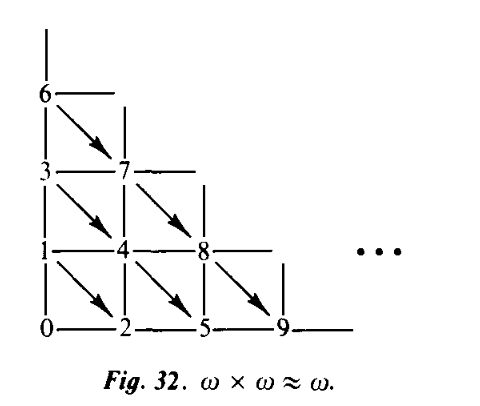
\includegraphics[width=0.6\textwidth]{fig-32}
      \centering
    \end{figure}
    Let $m, n \in \omega$.
    We note the next point following $(m, n)$ that coincides with the $x$-axis
      is $(m + n, 0)$.
    We can then formulate the sum of points seen as
      \begin{equation}
        \hyperlabel{sub:exercise-5-2-eq1}
        \left[ \sum_{i=0}^{m + n} (i + 1) \right] - n.
      \end{equation}
    All that remains is showing \eqref{sub:exercise-5-2-eq1} identifies with
      the equation for $J$.
    \eqref{sub:exercise-5-2-eq1} is an arithmetic series.
    By \nameref{S:sub:sum-arithmetic-series},
      \begin{align*}
        \left[ \sum_{i=0}^{m + n} (i + 1) \right] - n
          & = \frac{[(m + n) + 1][1 + (m + n + 1)]}{2} - n \\
          & = \frac{[(m + n) + 1][(m + n) + 2]}{2} - n \\
          & = \frac{(m + n)^2 + 2(m + n) + (m + n) - 2n}{2} \\
          & = \frac{1}{2}[(m + n)^2 + 3m + n] \\
          & = J(m, n).
      \end{align*}
    Hence $J$ is correctly defined.
  \end{proof}

\subsection{\unverified{Exercise 6.3}}%
\hyperlabel{sub:exercise-6.3}

  Find a one-to-one correspondence between the open unit interval $\ioo{0}{1}$
    and $\mathbb{R}$ that takes rationals to rationals and irrationals to
    irrationals.

  \begin{proof}

    \begin{figure}[ht]
      \label{sub:exercise-6-3-fig1}
      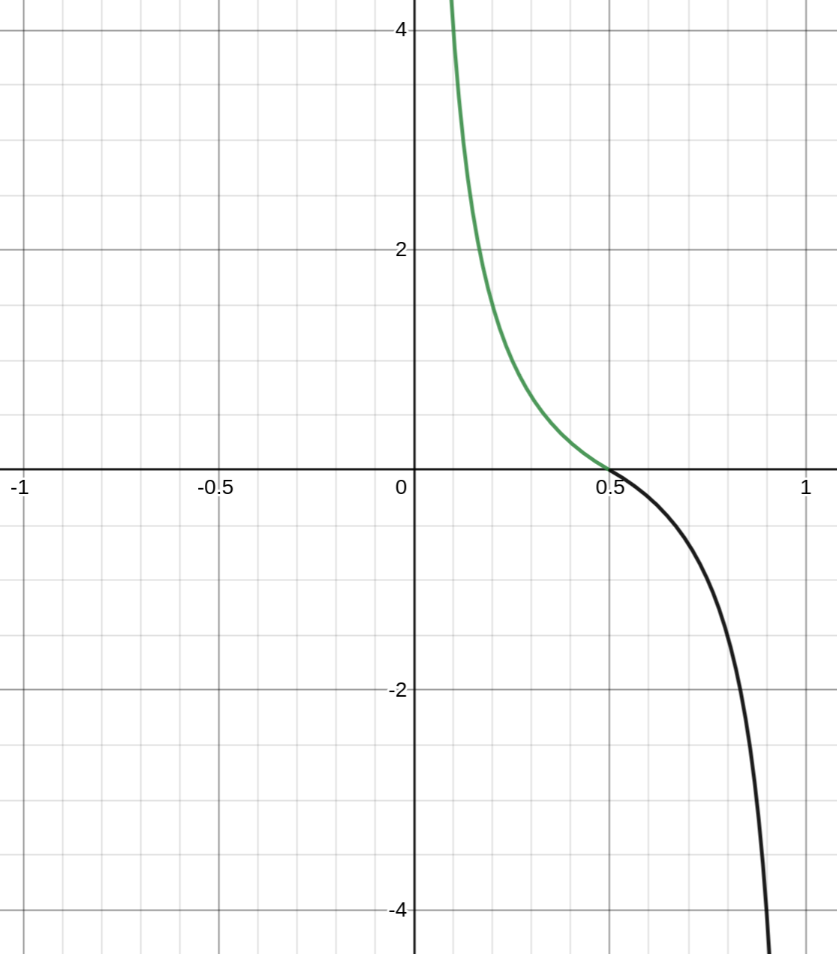
\includegraphics[width=0.6\textwidth]{exercise-6.3.png}
      \centering
    \end{figure}

    Consider function $f \colon (0, 1) \rightarrow \mathbb{R}$ given by
      $$f(x) = \begin{cases}
        \frac{1}{2x} - 1 & \text{if } x \leq \frac{1}{2} \\
        \frac{1}{2(x - 1)} + 1 & \text{otherwise}.
      \end{cases}$$
    We prove that (i) $f$ is a one-to-one into $\mathbb{R}$, (ii) $f$ is onto
      $\mathbb{R}$, and (iii) $f$ takes rationals to rationals and irrationals
      to irrationals.

    \paragraph{(i)}%

      Before proceeding, consider the solutions to the following identity:
        \begin{align*}
          \frac{1}{2x} - 1 = \frac{1}{2(x - 1)} + 1
          & \iff -8x^2 + 8x - 2 = 0 \\
          & \iff 4x^2 - 4x + 1 = 0.
        \end{align*}
      Applying the quadratic equation shows $x = 1 / 2$ is the only solution.
      Thus for any $x_1, x_2 \in \ioo{0}{1}$ such that $f(x_1) = f(x_2)$, it
        must be that $x_1, x_2 \leq 1 / 2$ or $x_1, x_2 > 1 / 2$.

      We now prove $f$ is one-to-one.
      Let $y \in \ran{f}$.
      Then there exists some $x_1 \in \ioo{0}{1}$ such that $f(x_1) = y$.
      Suppose there exists some $x_2 \in \ioo{0}{1}$ such that $f(x_1) = f(x_2)$.
      We prove that $x_1 = x_2$ by case analysis:

      \subparagraph{Case 1}%

        Suppose $x_1, x_2 \leq 1 / 2$.
        Then $$\frac{1}{2x_1} - 1 = \frac{1}{2x_2} - 1$$ which straightforwardly
          simplifies to $x_1 = x_2$.

      \subparagraph{Case 2}%

        Suppose $x_1, x_2 > 1 / 2$.
        Then $$\frac{1}{2(x_1 - 1)} + 1 = \frac{1}{2(x_2 - 1)} + 1$$ also
          straightfowardly simplies to $x_1 = x_2$.

      \subparagraph{Subconclusion}%

        The above cases are exhaustive.
        Therefore $f(x_1) = f(x_2)$ implies $x_1 = x_2$.
        Hence $f$ is one-to-one.

    \paragraph{(ii)}%

      Let $y \in \mathbb{R}$.
      We prove that there exists an $x \in (0, 1)$ such that $f(x) = y$.
      There are three cases we consider:

      \subparagraph{Case 1}%

        Suppose $y = 0$.
        Then $f(1 / 2) = 0 = y$ is a readily identifiable solution.

      \subparagraph{Case 2}%

        Suppose $y > 0$.
        Consider $x = \frac{1}{2(y + 1)}$.
        We note that $x < 1 / 2$ meaning
          \begin{align*}
            f(x)
              & = f\left(\frac{1}{2(y + 1)}\right) \\
              & = \frac{1}{2(\frac{1}{2(y + 1)})} - 1 \\
              & = (y + 1) - 1 \\
              & = y.
          \end{align*}

      \subparagraph{Case 3}%

        Suppose $y < 0$.
        Consider $x = \frac{1}{2(y - 1)} + 1$.
        We note that $x > 1 / 2$ meaning
          \begin{align*}
            f(x)
              & = f\left(\frac{1}{2(y - 1)} + 1\right) \\
              & = \frac{1}{2((\frac{1}{2(y - 1)} + 1) - 1)} + 1 \\
              & = (y - 1) + 1 \\
              & = y.
          \end{align*}

      \subparagraph{Subconclusion}%

        The above three cases are exhaustive.
        Thus $\ran{f} = \mathbb{R}$, i.e. $f$ is onto $\mathbb{R}$.

    \paragraph{(iii)}%

      Let $x \in (0, 1)$.
      There are two cases to consider:

      \subparagraph{Case 1}%

        Suppose $x$ is a rational number.
        Then there exist integers $m$ and $n$ such that $x = m / n$.
        If $x \leq 1 / 2$, then
          \begin{align*}
            f(x)
              & = f(m / n) \\
              & = \frac{1}{2\left(\frac{m}{n}\right)} - 1 \\
              & = \frac{n}{2m} - 1 \\
              & = \frac{n - 2m}{2m}.
          \end{align*}
        Since $n - 2m$ and $2m$ are integers, $f(x)$ is a rational number.
        If instead $x > 1 / 2$, then
          \begin{align*}
            f(x)
              & = f(m / n) \\
              & = \frac{1}{2\left(\frac{m}{n} - 1\right)} + 1 \\
              & = \frac{n}{2(m - n)} + 1 \\
              & = \frac{n + 2(m - n)}{2(m - n)}.
          \end{align*}
        Since $n + 2(m - n)$ and $2(m - n)$ are integers, $f(x)$ is again a
          rational number.
        Thus $f$ maps every rational number to a rational number.

      \subparagraph{Case 2}%

        Suppose $x$ is an irrational number.
        First, consider the case where $x \leq 1 / 2$ and, for the sake of
          contradiction, suppose $f(x)$ was a rational number.
        Then there exist integers $m$ and $n$ such that
          $$f(x) = \frac{1}{2x} - 1 = \frac{m}{n}.$$
        But this would imply $$x = \frac{n}{2(m + n)},$$ a contradiction.
        Thus $f(x)$ must be irrational.

        Likewise, consider the case where $x > 1 / 2$.
        Again, for the sake of contradiction, suppose $f(x)$ was a rational
          number.
        Then there exist integers $m$ and $n$ such that
          $$f(x) = \frac{1}{2(x - 1)} + 1 = \frac{m}{n}.$$
        But this would imply $$x = \frac{n}{2(m - n)} + 1,$$ a contradiction.
        Thus $f(x)$ must be irrational.

        Hence $f$ maps every irrational number to an irrational number.

  \end{proof}

\subsection{\sorry{Exercise 6.4}}%
\hyperlabel{sub:exercise-6.4}

  Construct a one-to-one correspondence between the closed unit interval
    $$\icc{0}{1} = \{x \in \mathbb{R} \mid 0 \leq x \leq 1\}$$
    and the open unit interval $\ioo{0}{1}$.

  \begin{proof}
    TODO
  \end{proof}

\subsection{\verified{Exercise 6.5}}%
\hyperlabel{sub:exercise-6.5}

  Prove \nameref{sub:theorem-6a}.

  \begin{proof}
    Refer to \nameref{sub:theorem-6a}.
  \end{proof}

\subsection{\sorry{Exercise 6.6}}%
\hyperlabel{sub:exercise-6.6}

  Let $\kappa$ be a nonzero cardinal number.
  Show there does not exist a set to which every set of cardinality $\kappa$
    belongs.

  \begin{proof}
    TODO
  \end{proof}

\subsection{\sorry{Exercise 6.7}}%
\hyperlabel{sub:exercise-6.7}

  Assume that $A$ is finite and $f \colon A \rightarrow A$.
  Show that $f$ is one-to-one iff $\ran{f} = A$.

  \begin{proof}
    TODO
  \end{proof}

\subsection{\sorry{Exercise 6.8}}%
\hyperlabel{sub:exercise-6.8}

  Prove that the union of two finite sets is finite, without any use of
    arithmetic.

  \begin{proof}
    TODO
  \end{proof}

\subsection{\sorry{Exercise 6.9}}%
\hyperlabel{sub:exercise-6.9}

  Prove that the Cartesian product of two finite sets is finite, without any use
    of arithmetic.

  \begin{proof}
    TODO
  \end{proof}

\subsection{\sorry{Exercise 6.10}}%
\hyperlabel{sub:exercise-6.10}

  Prove part 4 of \nameref{sub:theorem-6i}.

  \begin{proof}
    TODO
  \end{proof}

\subsection{\sorry{Exercise 6.11}}%
\hyperlabel{sub:exercise-6.11}

  Prove part 5 of \nameref{sub:theorem-6i}.

  \begin{proof}
    TODO
  \end{proof}

\subsection{\sorry{Exercise 6.12}}%
\hyperlabel{sub:exercise-6.12}

  The proof to \nameref{sub:theorem-6i} involves eight instances of showing two
    sets to be equinumerous.
  (The eight are listed in the proof of the theorem as statements numbered 1-6.)
  In which of these eight cases does equality actually hold?

  \begin{proof}
    TODO
  \end{proof}

\subsection{\sorry{Exercise 6.13}}%
\hyperlabel{sub:exercise-6.13}

  Show that a finite union of finite sets is finite.
  That is, show that if $B$ is a finite set whose members are themselves finite
    sets, then $\bigcup{B}$ is finite.

  \begin{proof}
    TODO
  \end{proof}

\subsection{\sorry{Exercise 6.14}}%
\hyperlabel{sub:exercise-6.14}

  Define a \textit{permutation} of $K$ to be any one-to-one function from $K$
    onto $K$.
  We can the define the factorial operation on cardinal numbers by the equation
    $$\kappa! = \card{\{f \mid f \text{ is a permutation of } K\}},$$
    where $K$ is any set of cardinality $\kappa$.
  Show that $\kappa!$ is well defined, i.e. the value of $\kappa!$ is
    independent of just which set $K$ is chosen.

  \begin{proof}
    TODO
  \end{proof}

\end{document}
